\cleardoublepage%
\refstepcounter{chapter}%
\phantomsection
\chapter[Appendix B - Supplemental Material]{\chaptermark{Appendix B}\label{chap:apx_B}Appendix B\\
Supplemental Material}%
\section{\label{app:DL}DL channel}
\newpage
\begin{figure}[H]
    \centering
    \begin{subfigure}{0.49\textwidth}
        \centering
        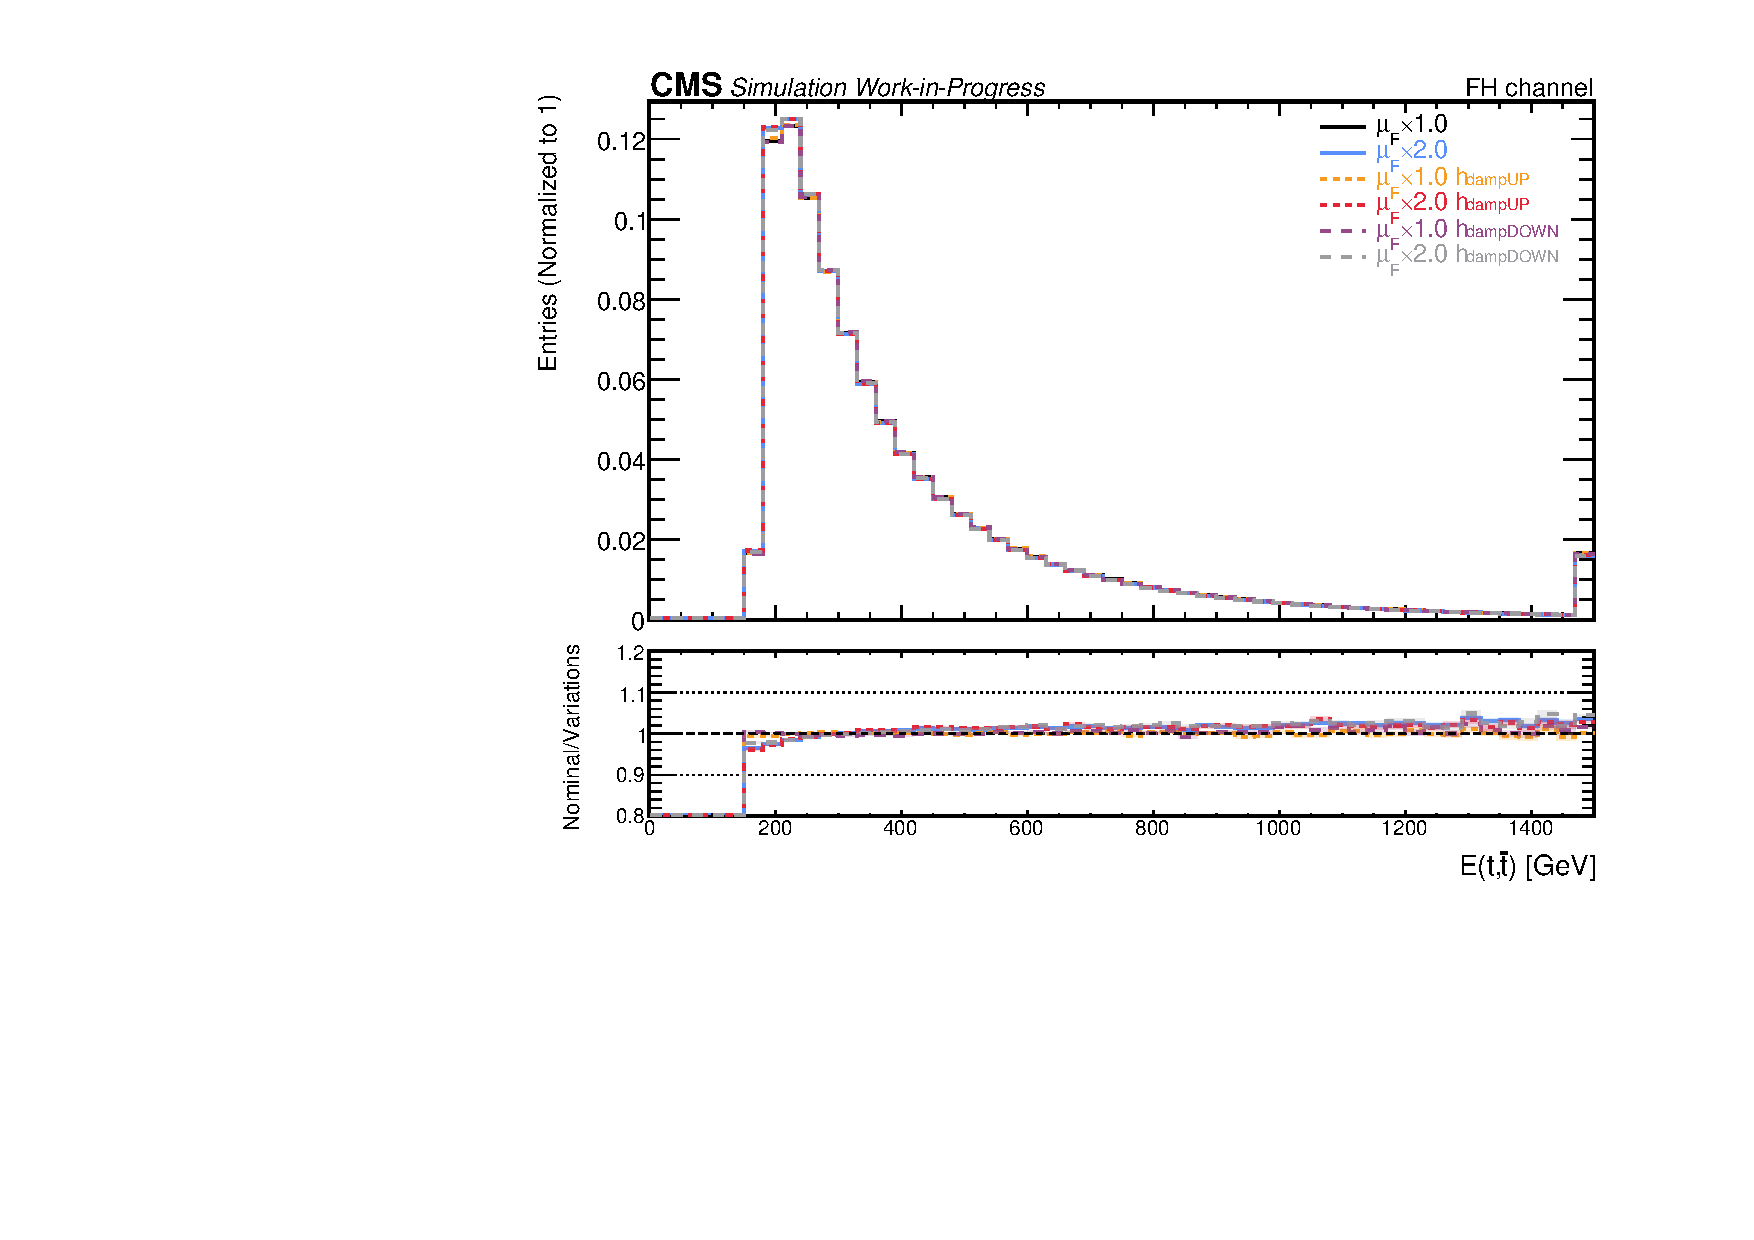
\includegraphics[width= 1.1\linewidth]{DL/ratio_ttbar_energy.pdf}
        \caption{}
        \label{app:subfig:E(t,tbar)_DL}
    \end{subfigure}
    \begin{subfigure}{0.48\textwidth}
        \centering
        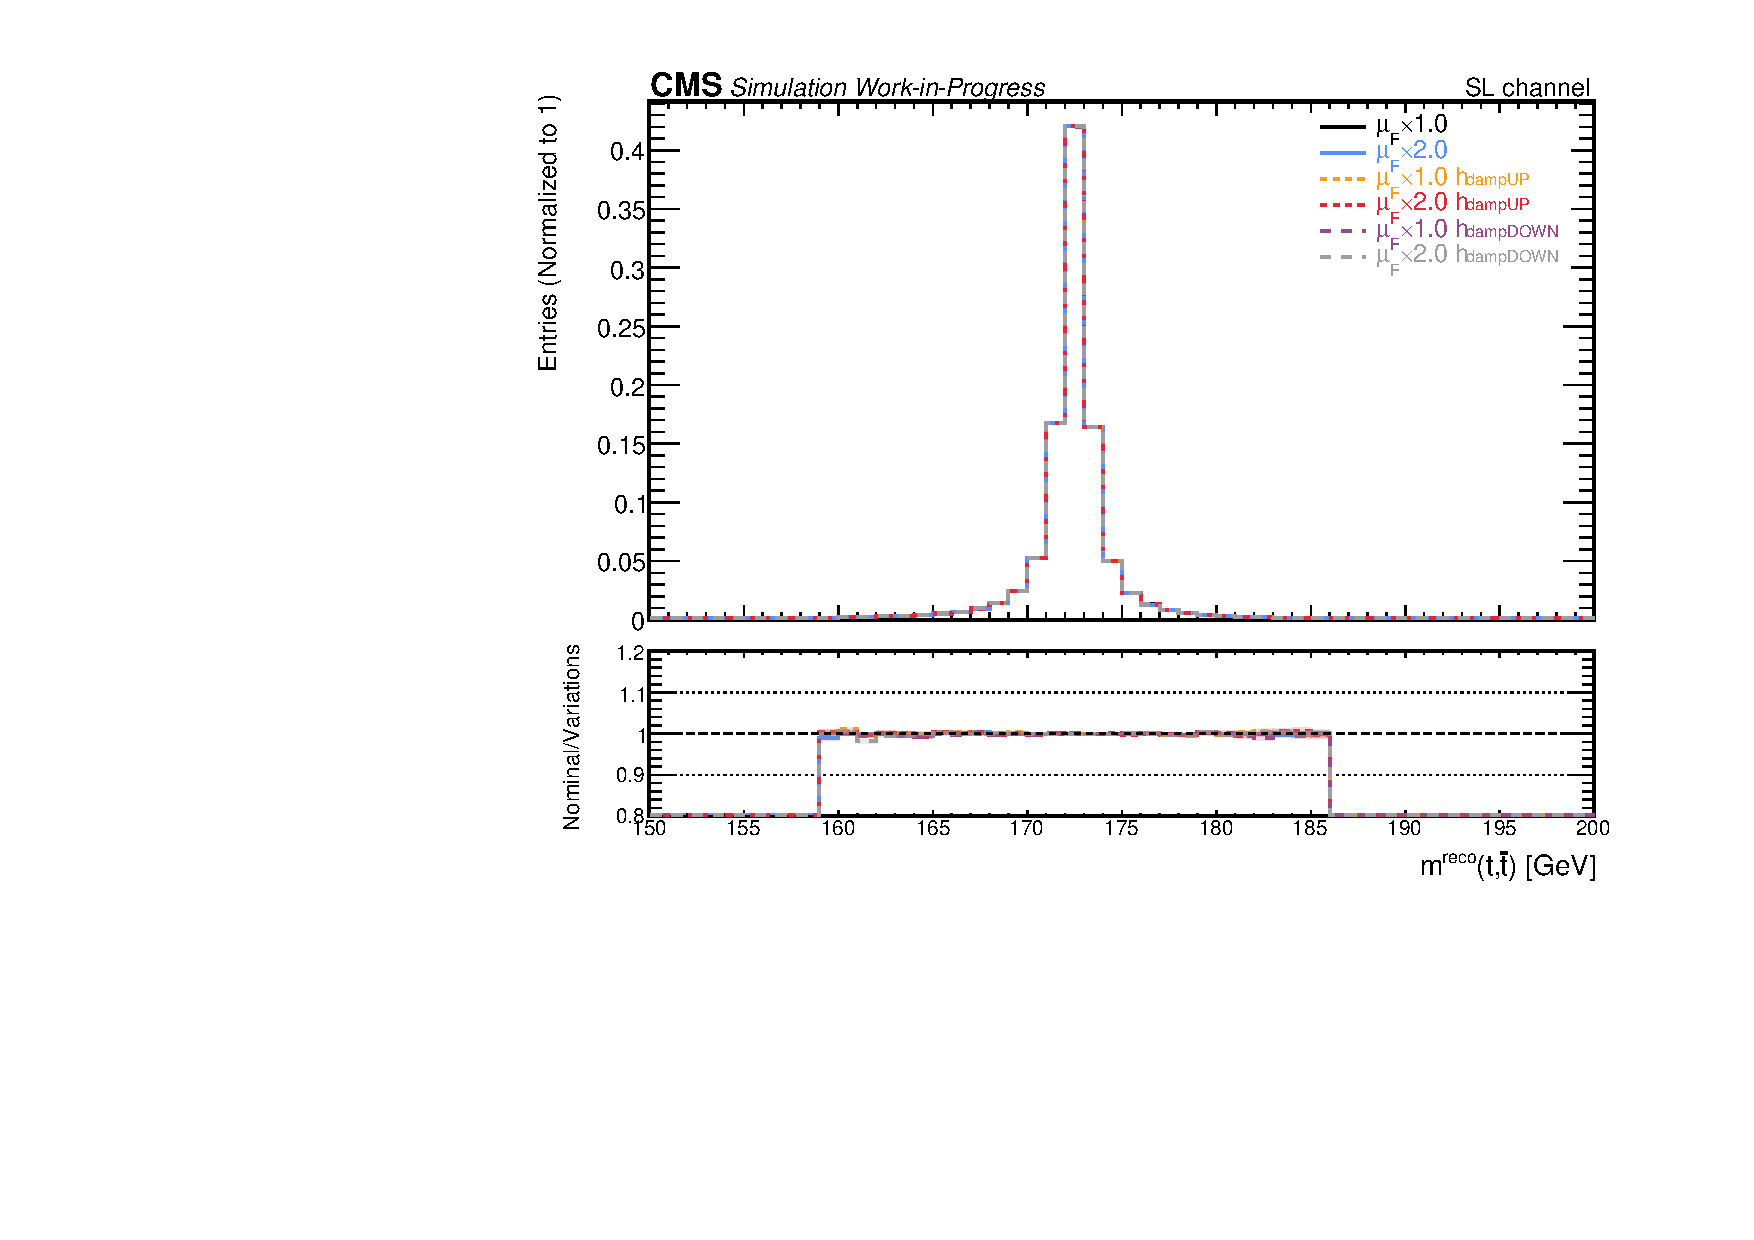
\includegraphics[width= 1.1\linewidth]{DL/ratio_ttbar_reco_mass.pdf}
        \caption{}
        \label{app:subfig:m(t,tbar)_DL}
    \end{subfigure}

    \vspace{0.2cm}
    
    \begin{subfigure}{0.49\textwidth}
        \centering
        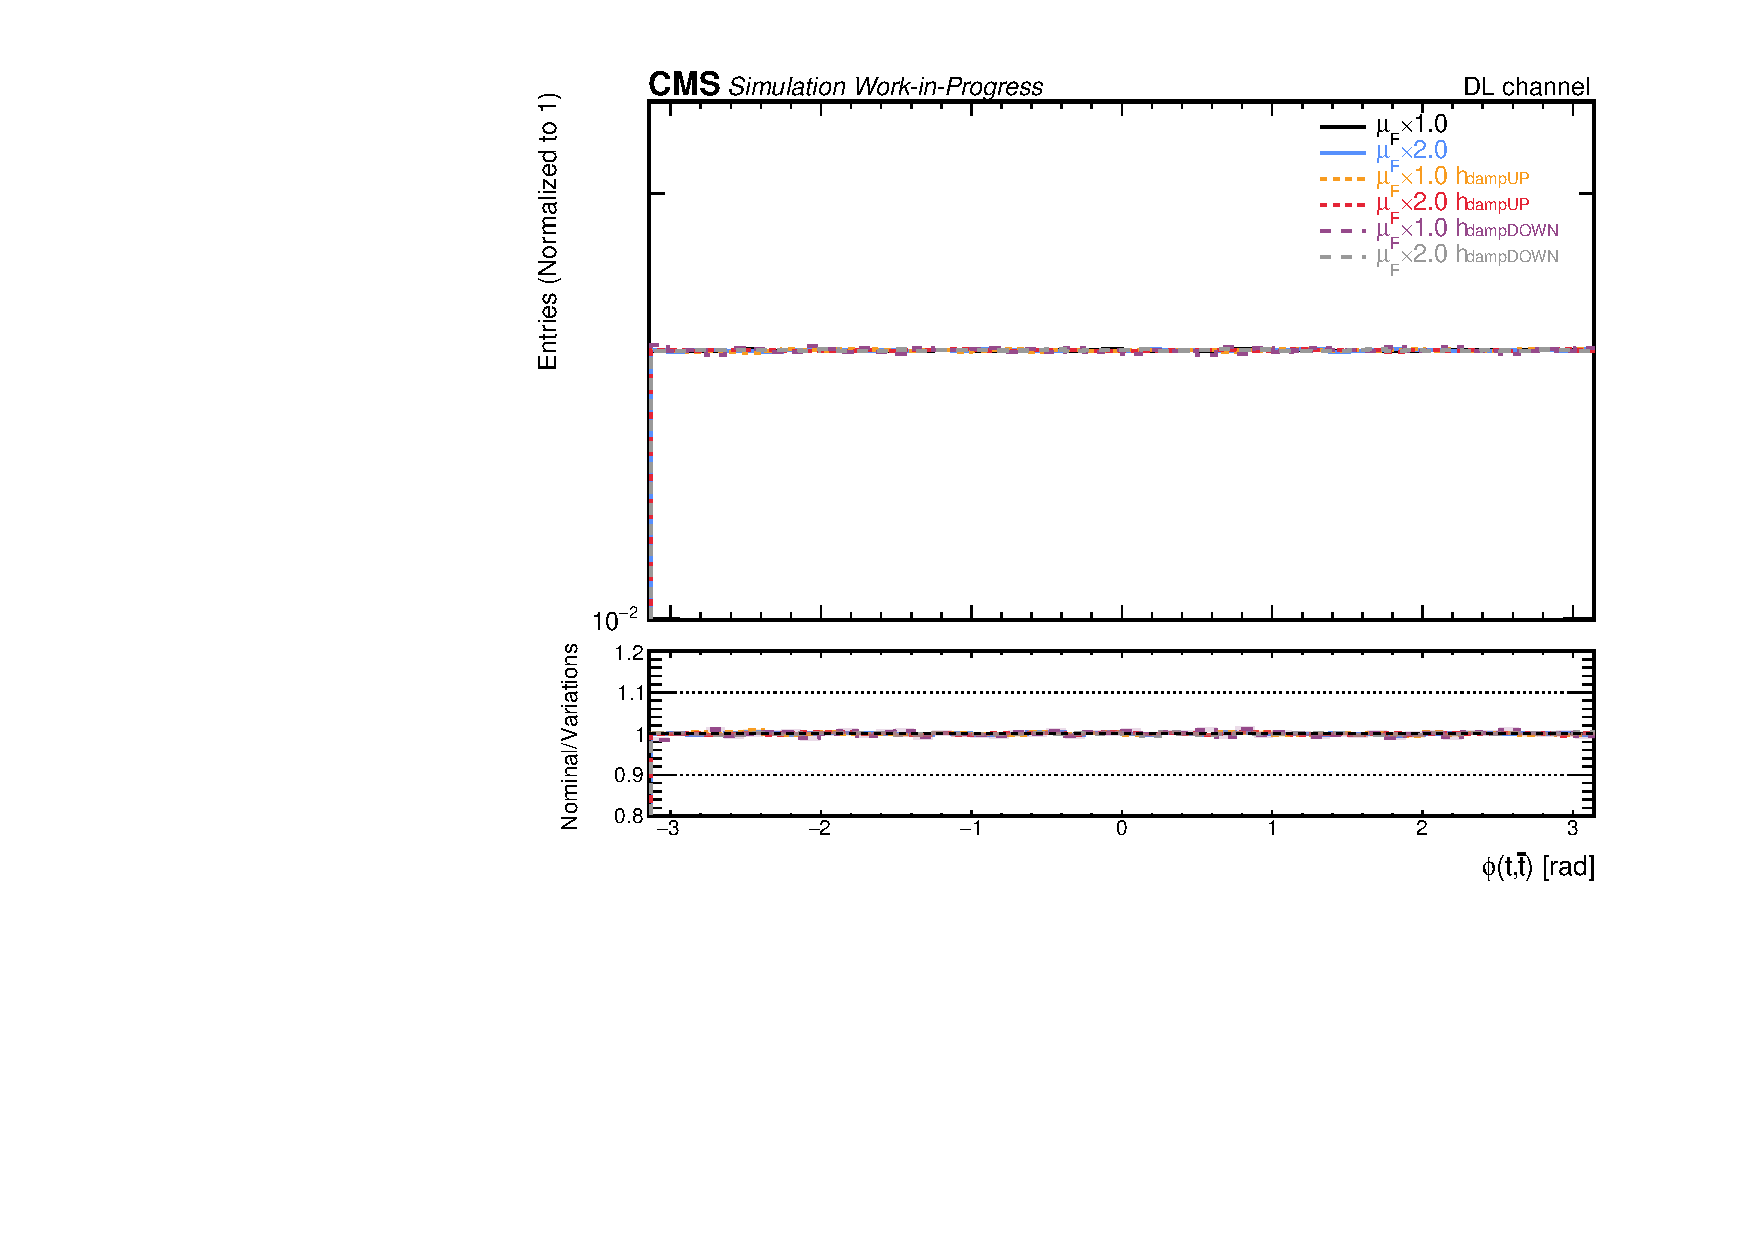
\includegraphics[width= 1.1\linewidth]{DL/ratio_ttbar_phi.pdf}
        \caption{}
        \label{app:subfig:phi(t,tbar)_DL}
    \end{subfigure}
    \begin{subfigure}{0.49\textwidth}
        \centering
        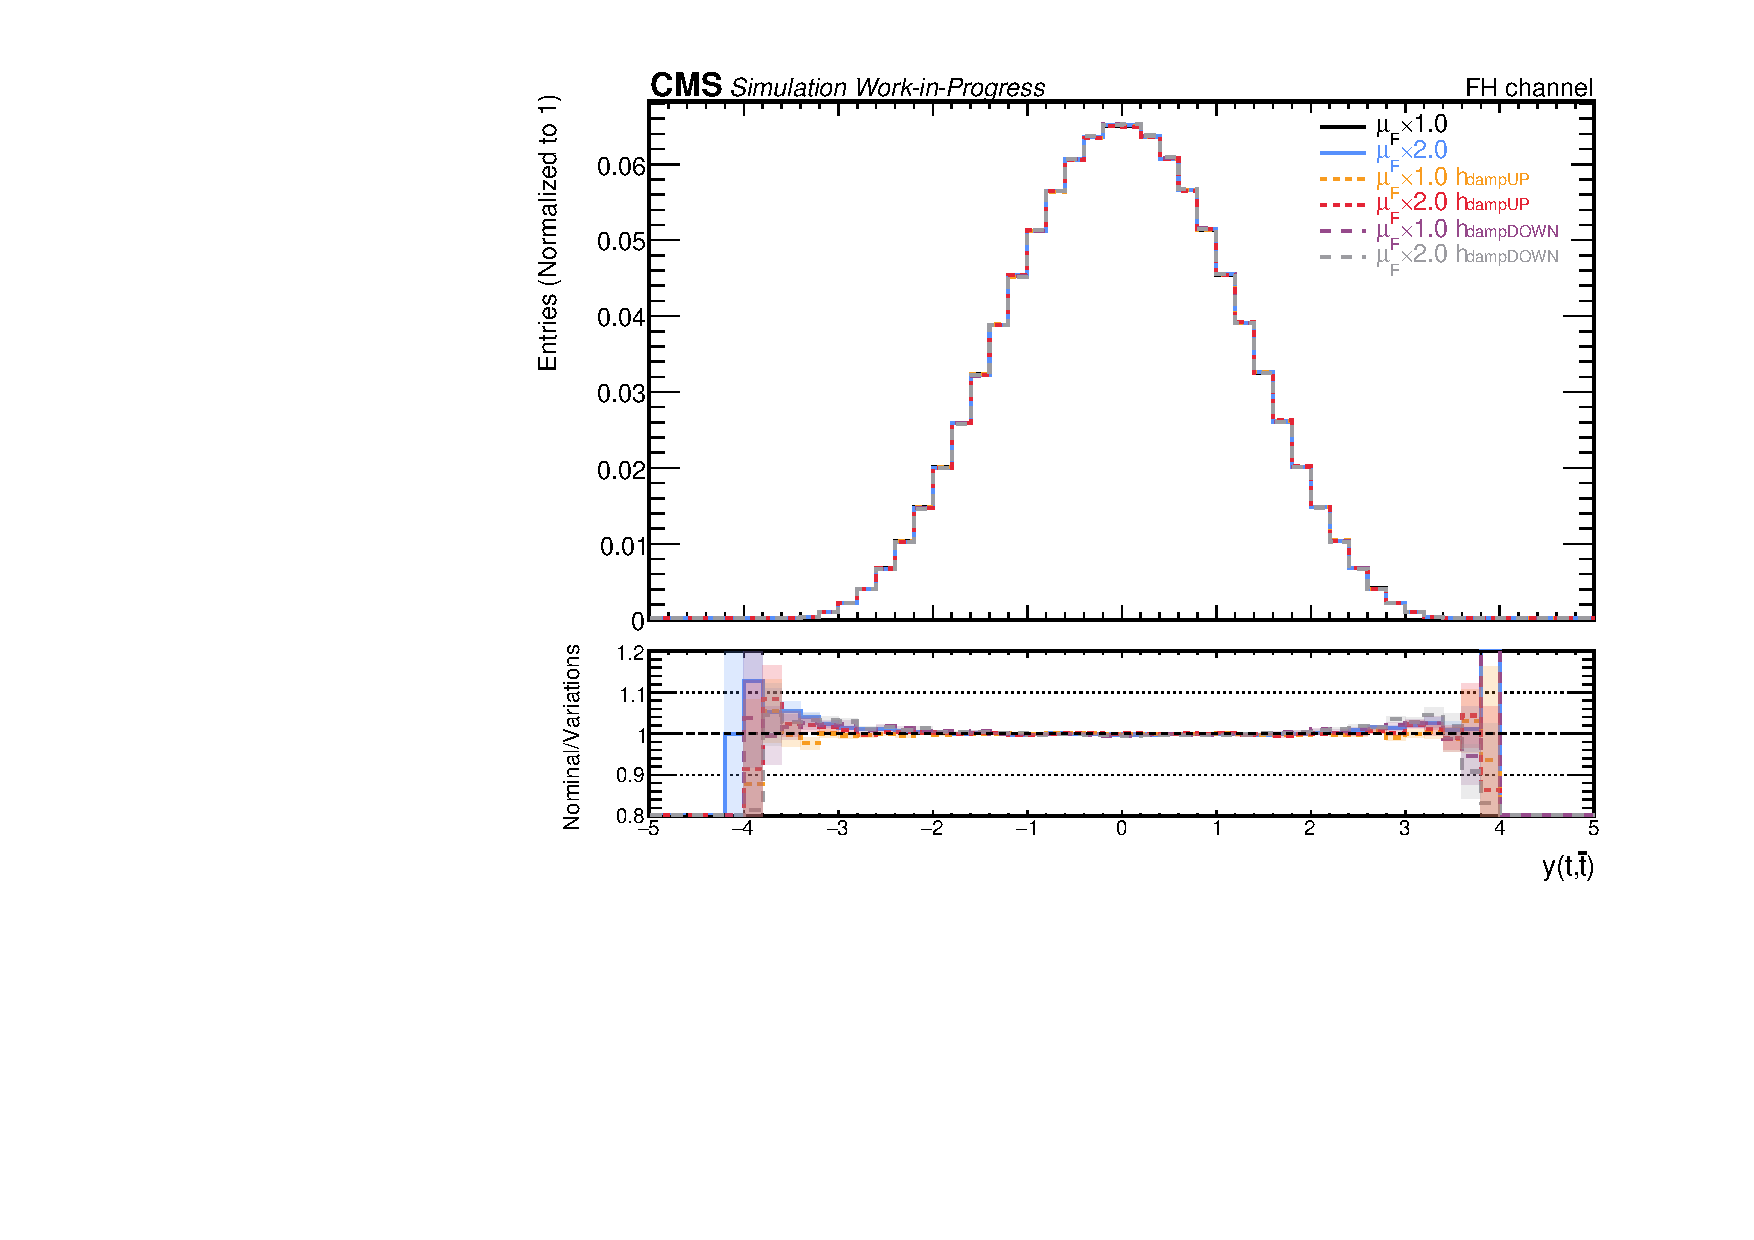
\includegraphics[width= 1.1\linewidth]{DL/ratio_ttbar_rapidity.pdf}
        \caption{}
        \label{app:subfig:y(t,tbar)_DL}
    \end{subfigure}
    
    \caption{Distributions of (a) energy, (b) reconstructed mass, (c) azimuthal angle and (d) rapidity of the t/$\overline{\text{t}}$ quarks for the six different settings used in the simulation. The lower panel shows the ratio of the nominal setting to the variations. The shaded bands represent statistical uncertainties. The last bins contain the overflow events.}
    \label{app:fig:t,tbar_DL}
\end{figure}


\begin{figure}[H]
    \centering
    \begin{subfigure}{0.49\textwidth}
        \centering
        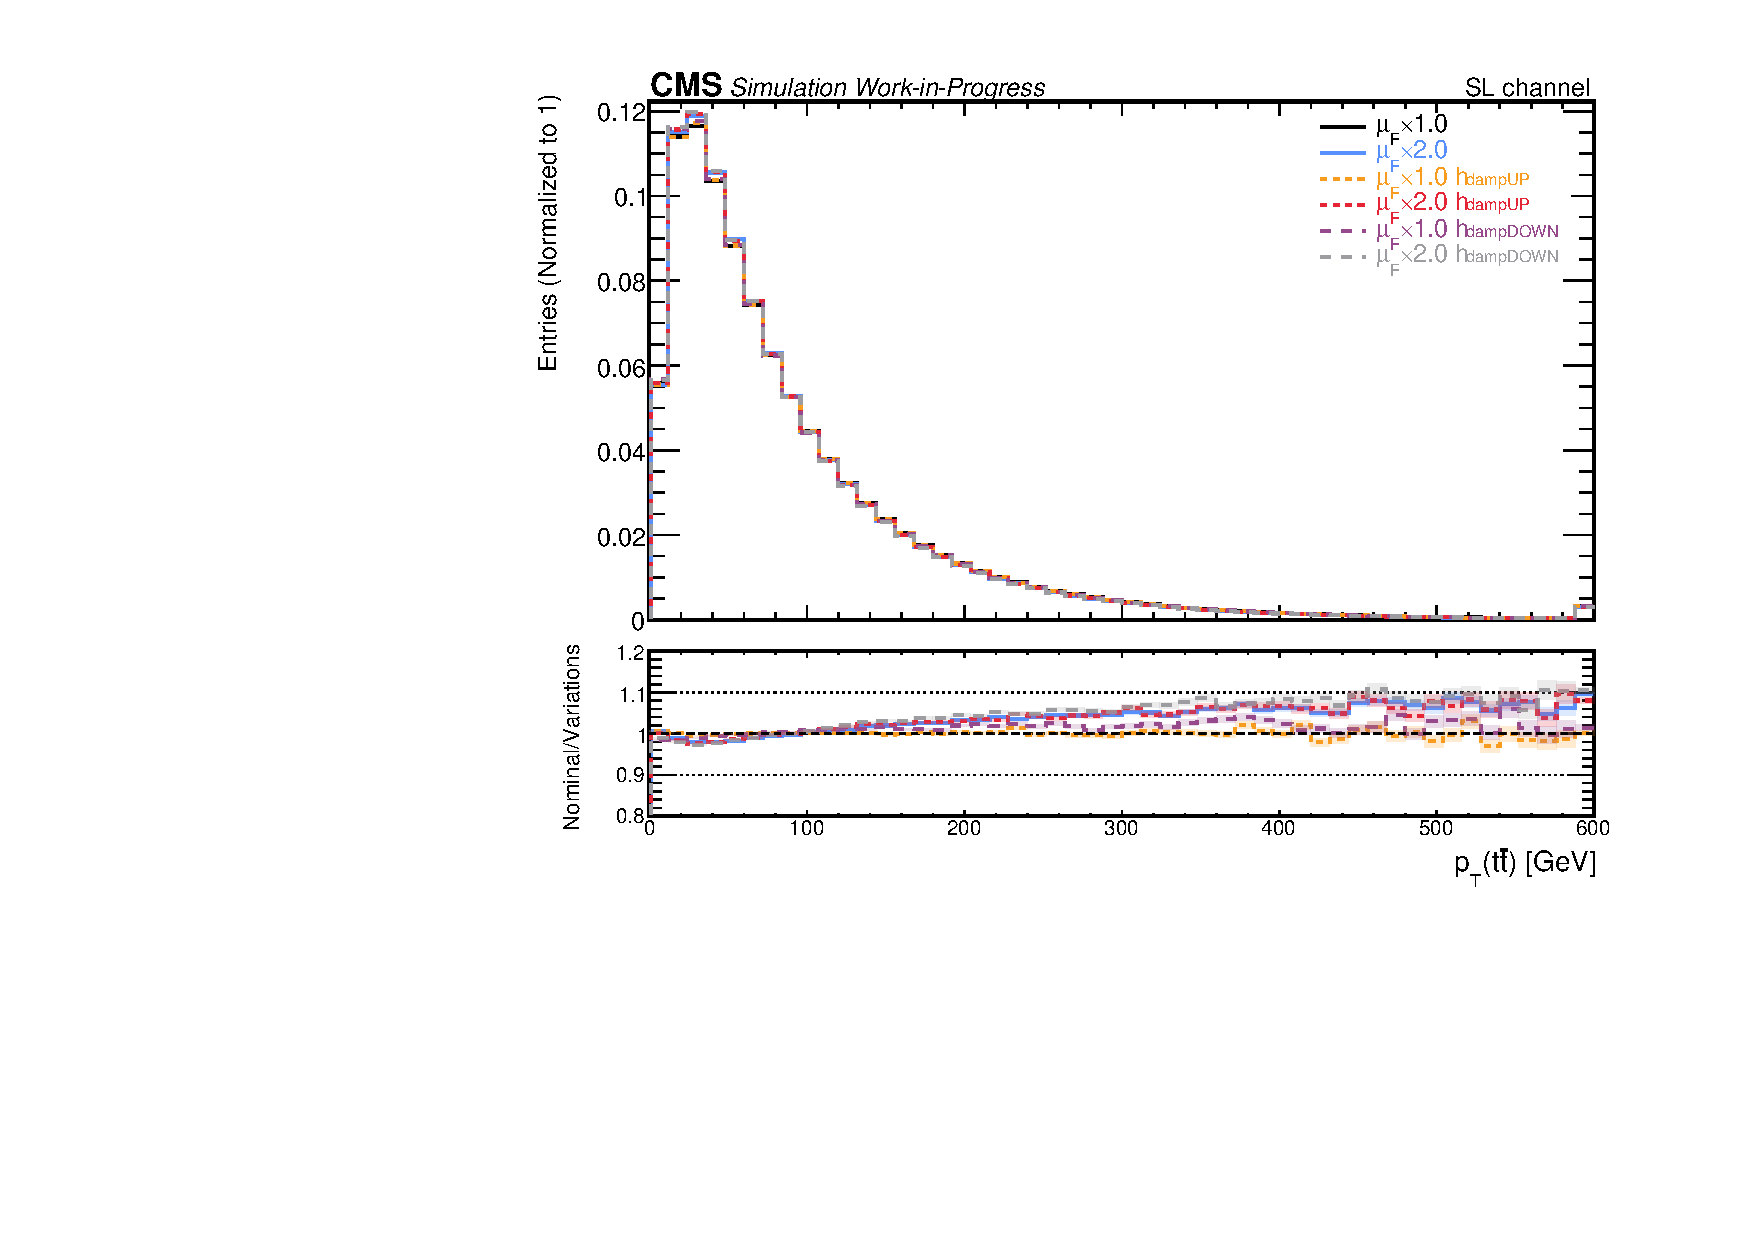
\includegraphics[width= 1.1\linewidth]{DL/ratio_tt_system_pt.pdf}
        \caption{}
        \label{app:subfig:pt(ttbar)_DL}
    \end{subfigure}
    \begin{subfigure}{0.49\textwidth}
        \centering
        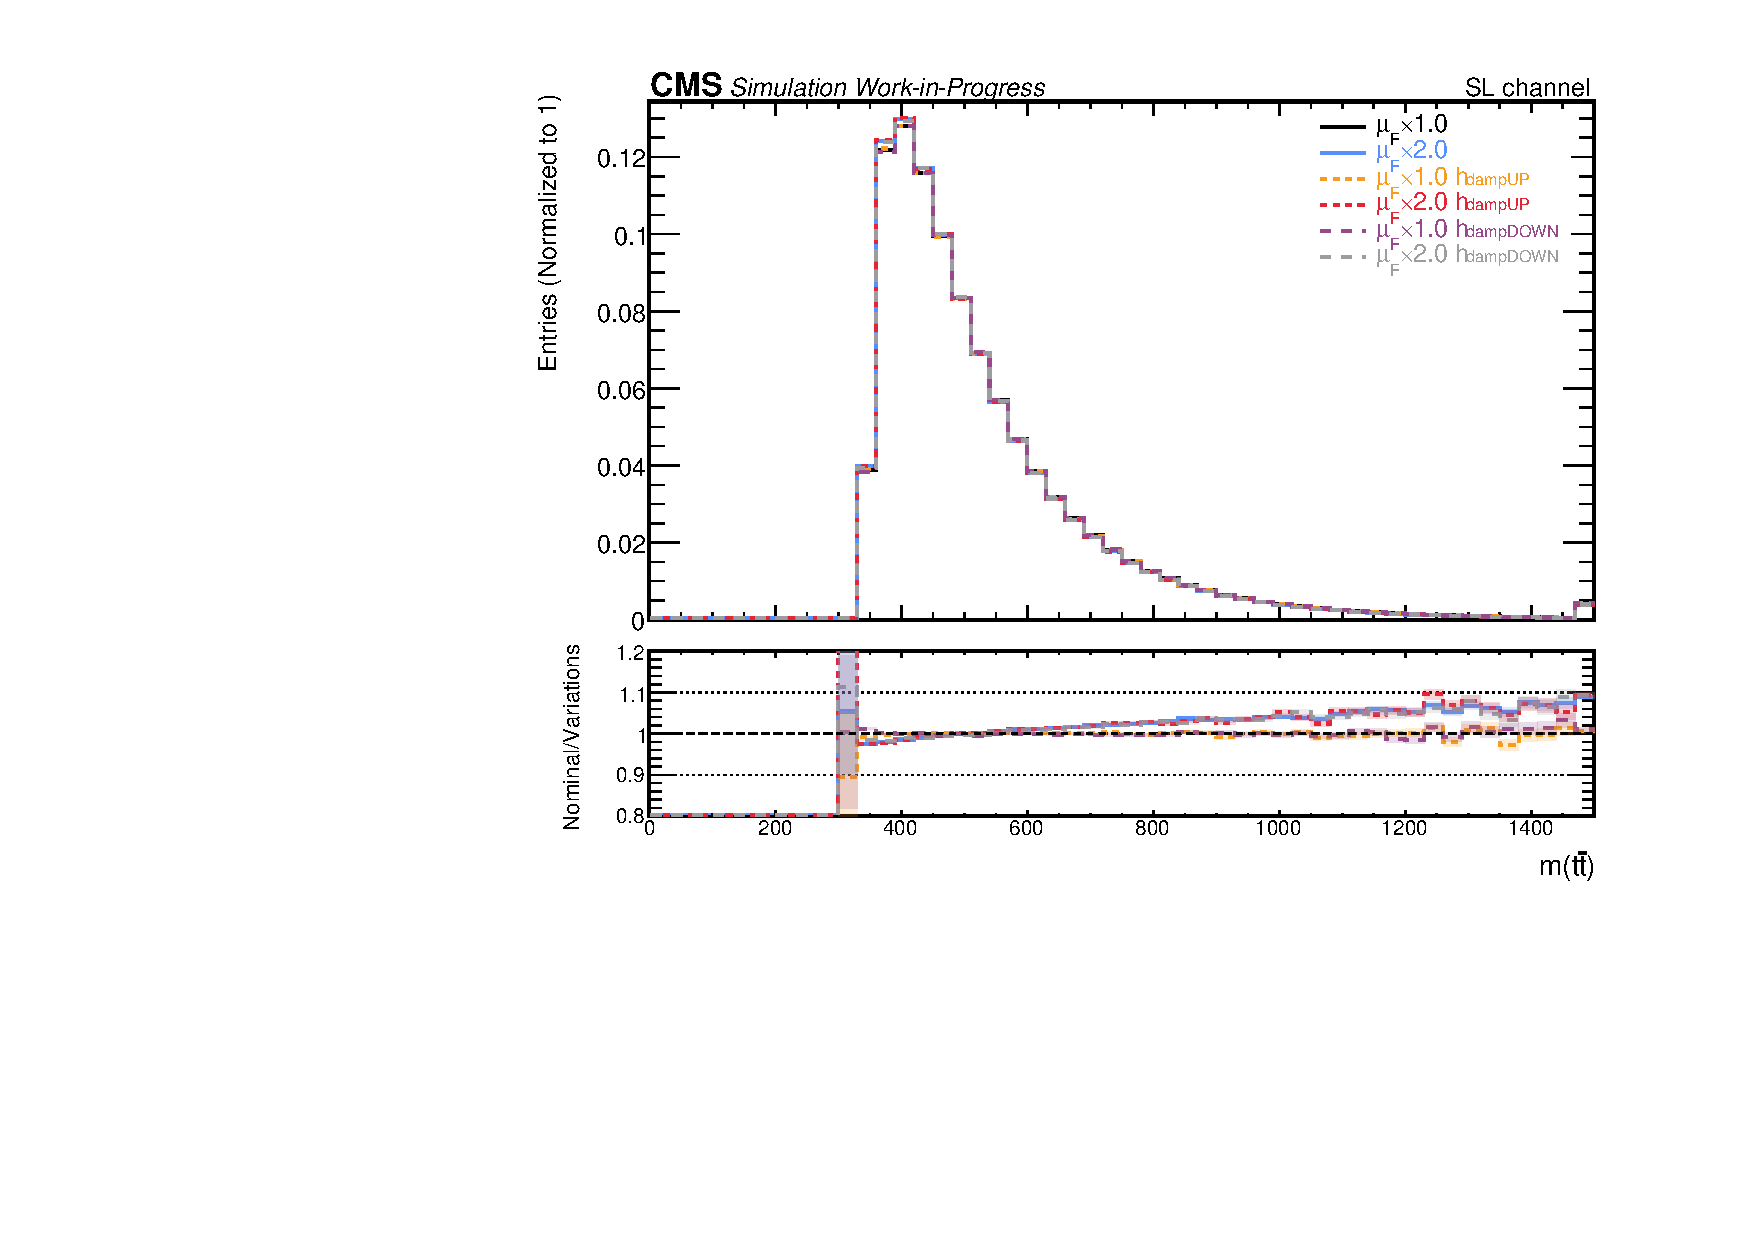
\includegraphics[width= 1.1\linewidth]{DL/ratio_tt_system_invariant_mass.pdf}
        \caption{}
        \label{app:subfig:m(ttbar_DL}
    \end{subfigure}

    \vspace{0.2cm}
    
    \begin{subfigure}{0.49\textwidth}
        \centering
        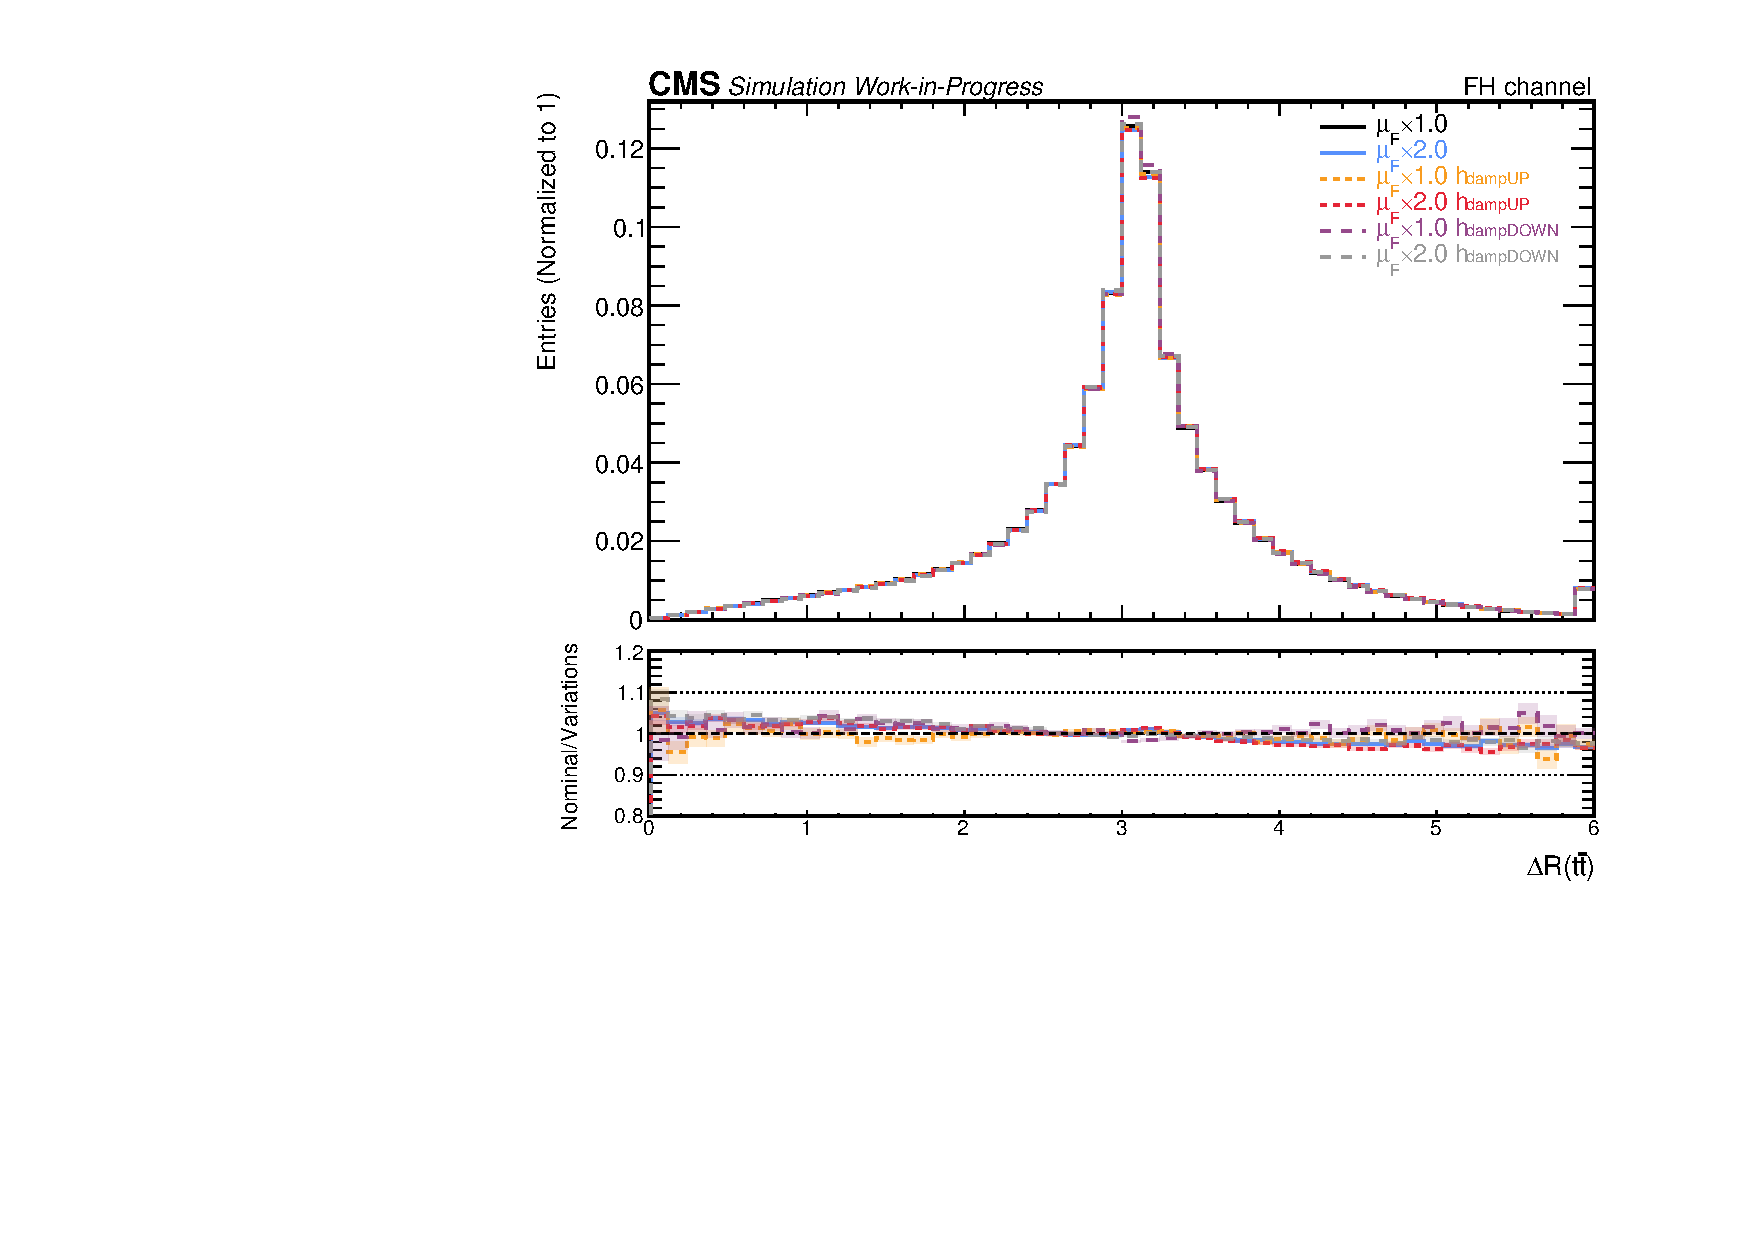
\includegraphics[width= 1.1\linewidth]{DL/ratio_tt_system_dR.pdf}
        \caption{}
        \label{app:subfig:dR(ttbar)_DL}
    \end{subfigure}
    \begin{subfigure}{0.49\textwidth}
        \centering
        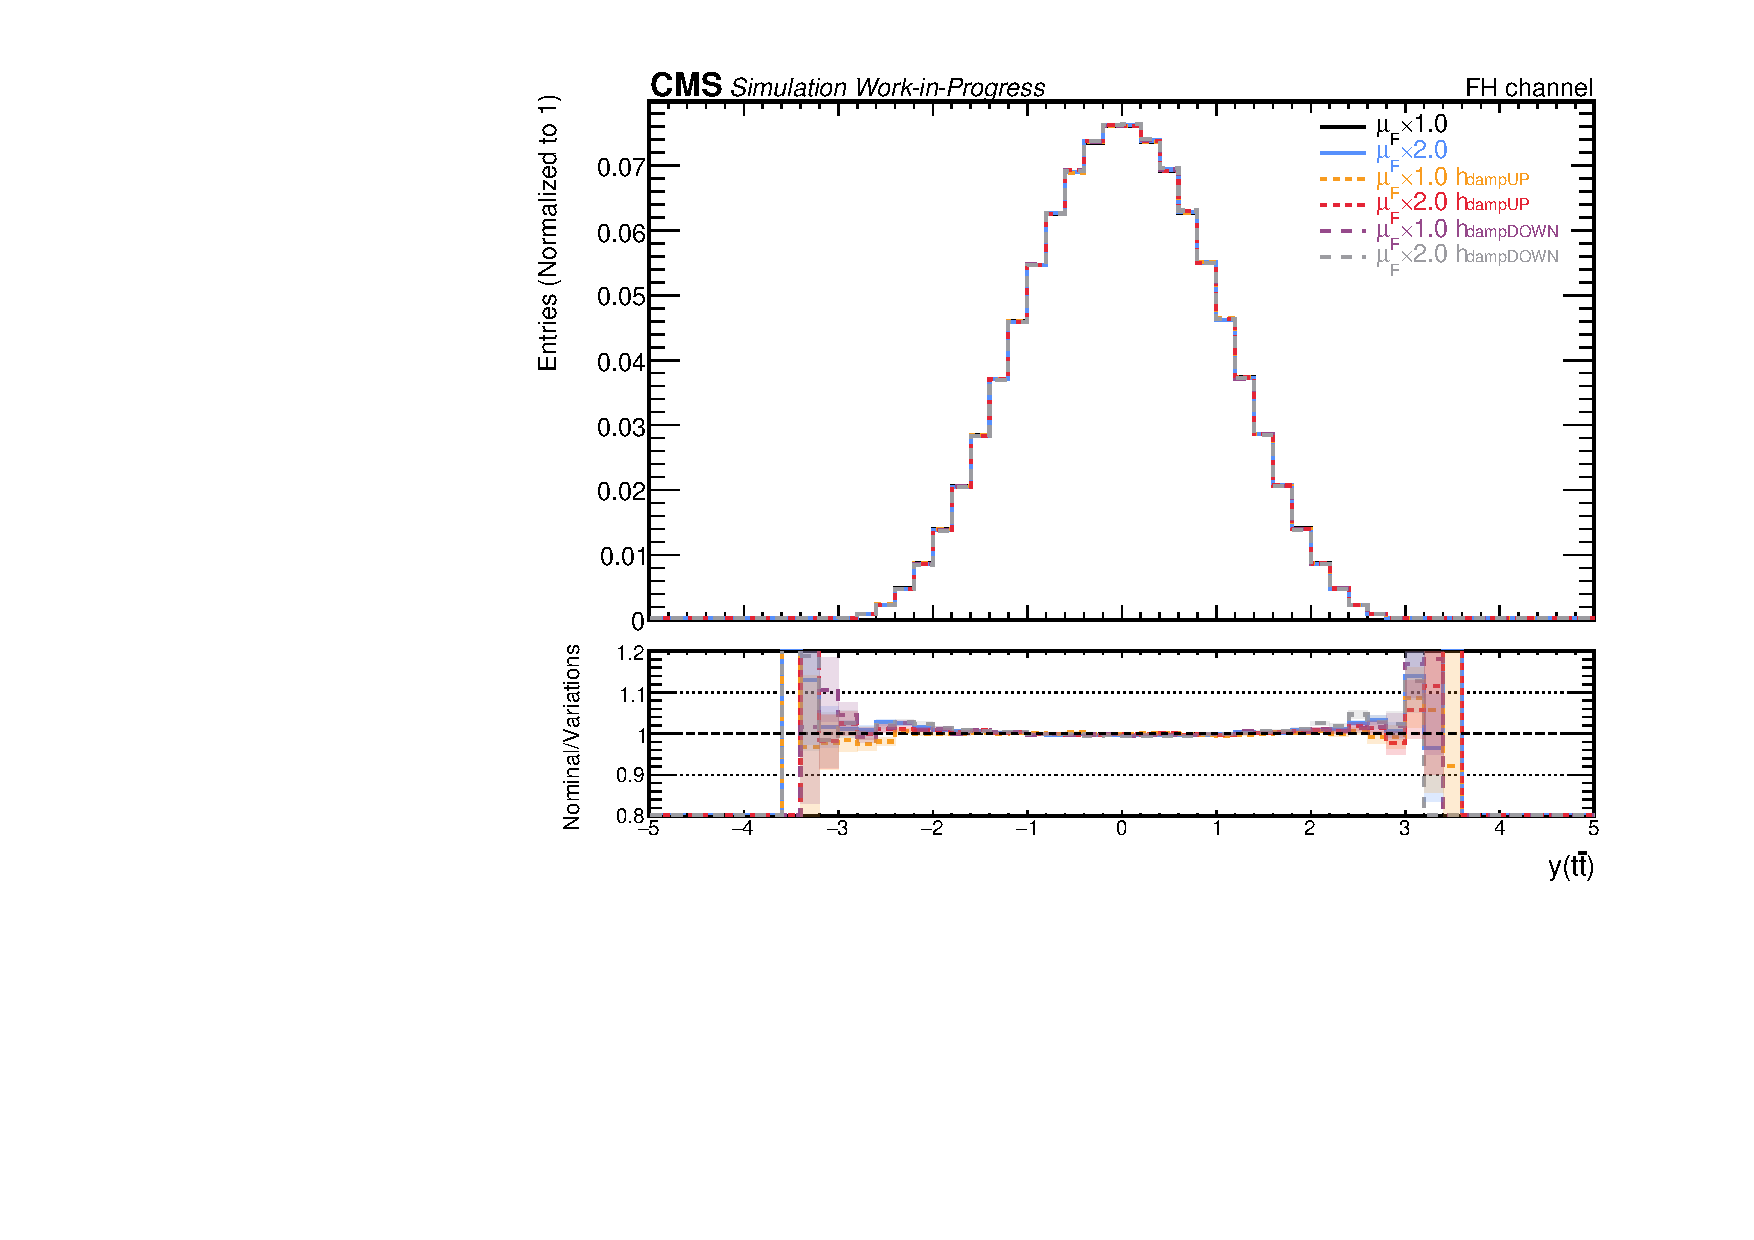
\includegraphics[width= 1.1\linewidth]{DL/ratio_tt_system_rapidity.pdf}
        \caption{}
        \label{app:subfig:y(ttbar)_DL}
    \end{subfigure}
    \caption{Distributions of (a) transverse momentum, (b) invariant mass,  (c) angular separation and (d) rapidity of the t$\overline{\text{t}}$ system for the six different settings used in the simulation. The lower panel shows the ratio of the nominal setting to the variations. The shaded bands represent statistical uncertainties. The last bins contain the overflow events.}
    \label{app:fig:ttbar_DL}
\end{figure}


\begin{figure}[H]
    \centering
    \begin{subfigure}{0.49\textwidth}
        \centering
        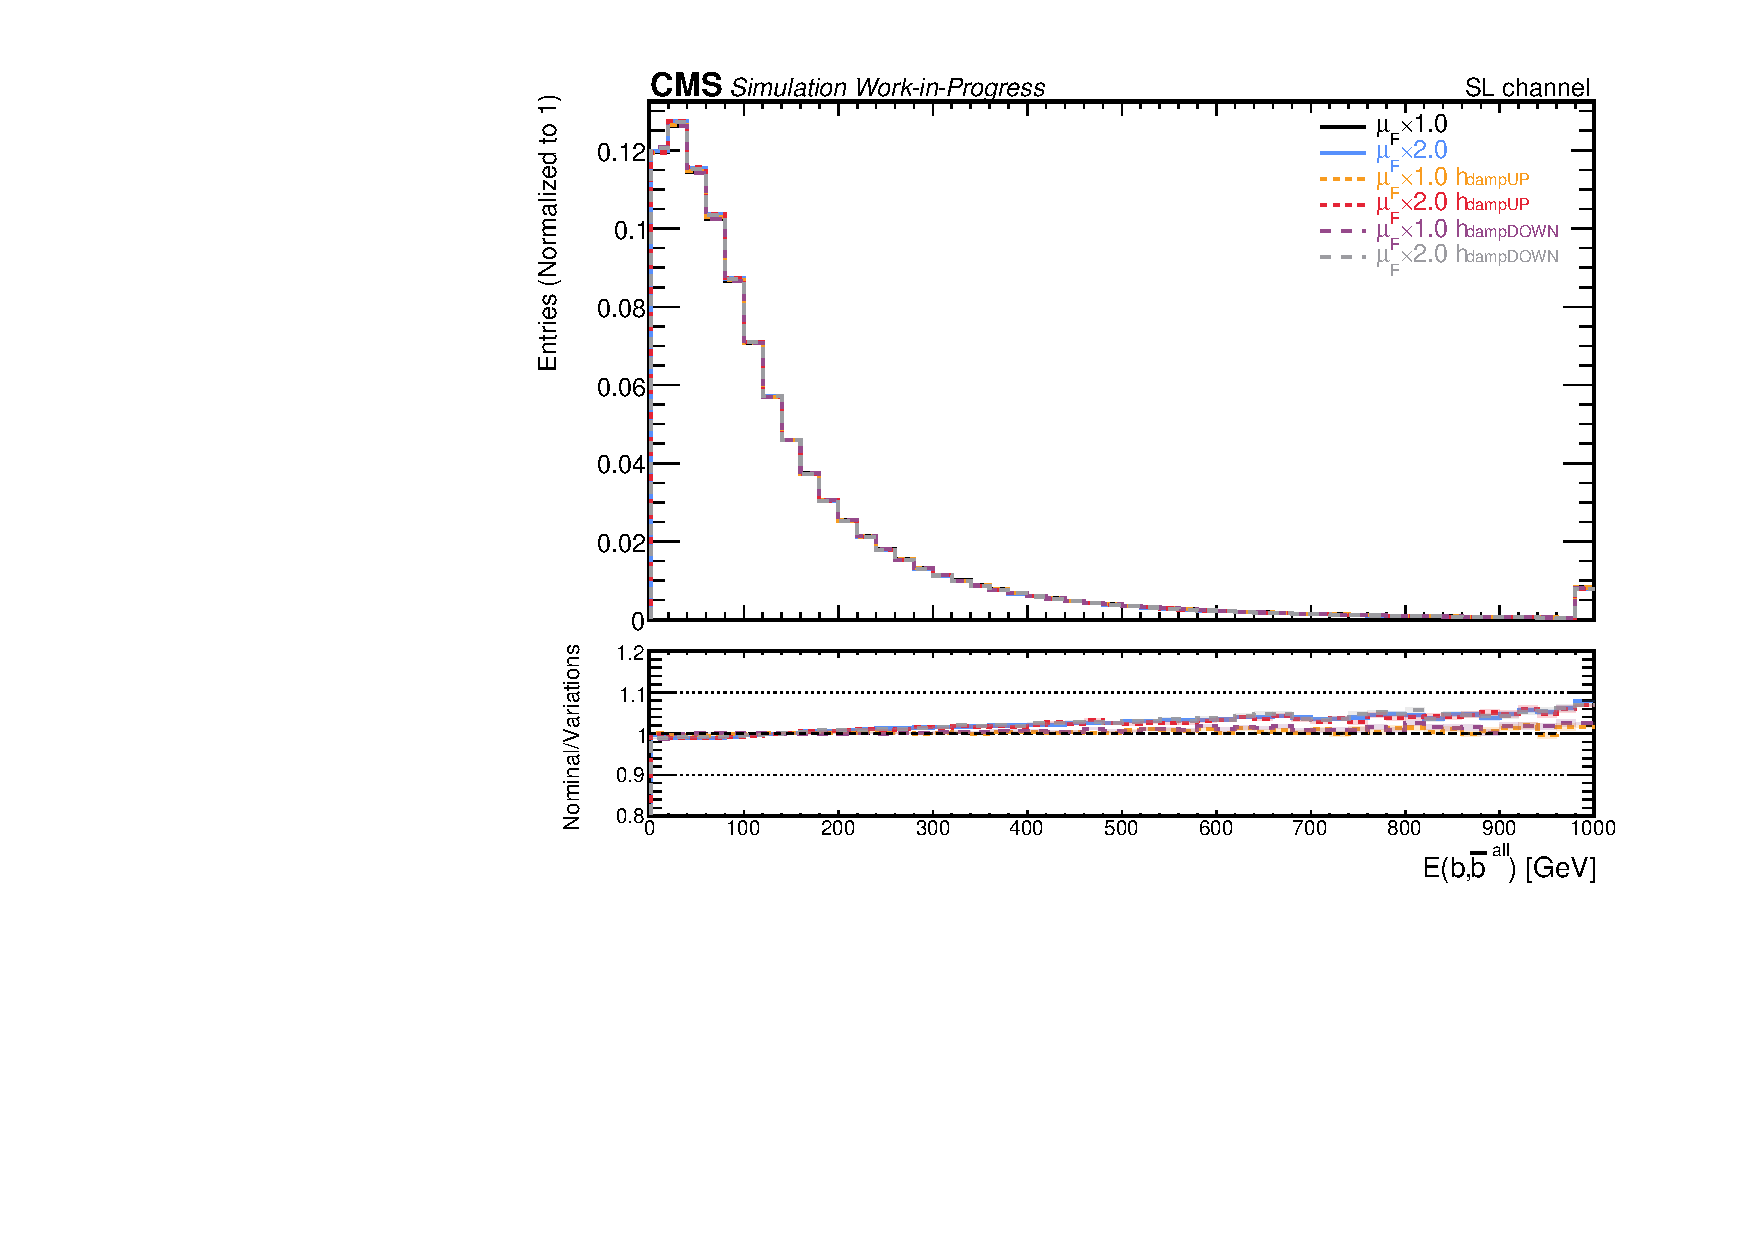
\includegraphics[width= 1.1\linewidth]{DL/ratio_b_all_energy.pdf}
        \caption{}
        \label{app:subfig:Ε(b_all)_DL}
    \end{subfigure}
    \begin{subfigure}{0.49\textwidth}
        \centering
        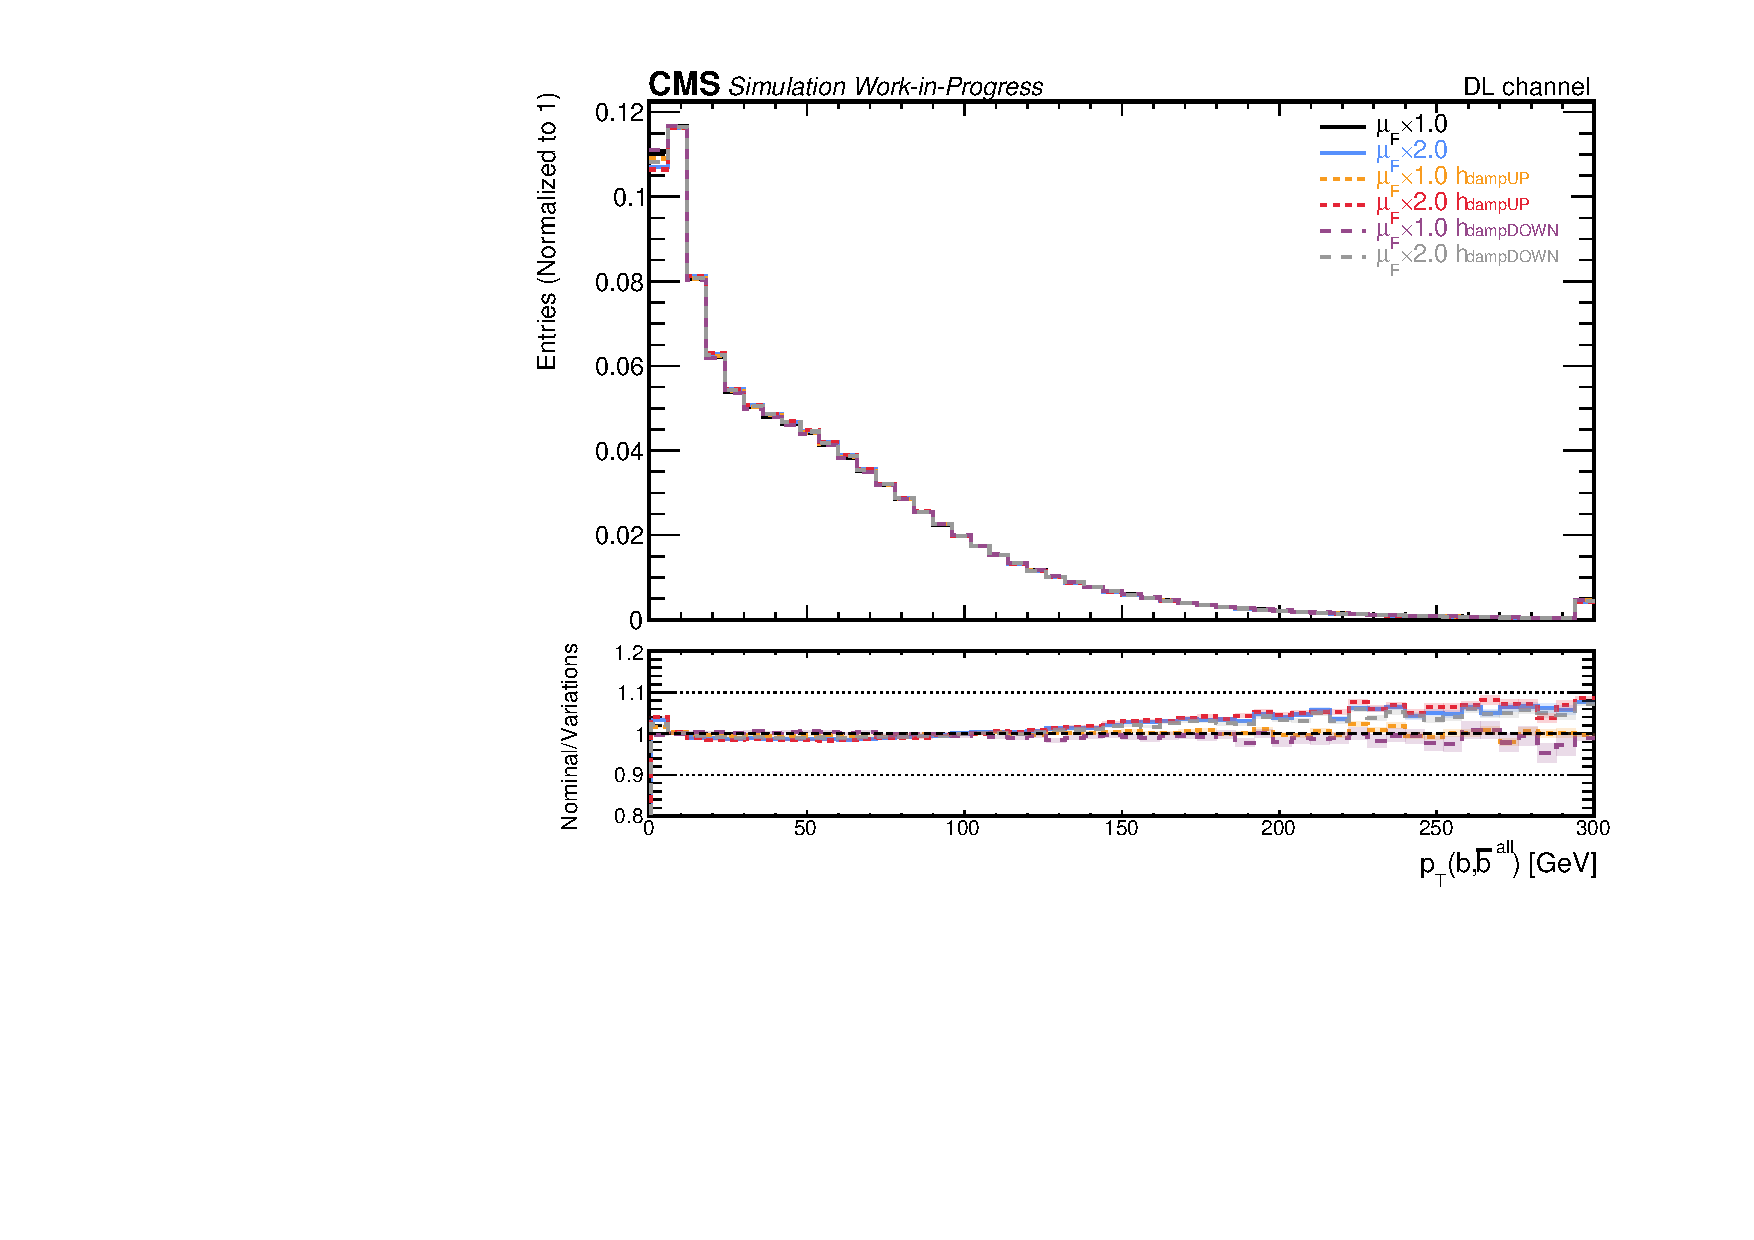
\includegraphics[width= 1.1\linewidth]{DL/ratio_b_all_pt.pdf}
        \caption{}
        \label{app:subfig:pt(b_all)_DL}
    \end{subfigure}

    \vspace{0.2cm}
    
    \begin{subfigure}{0.49\textwidth}
        \centering
        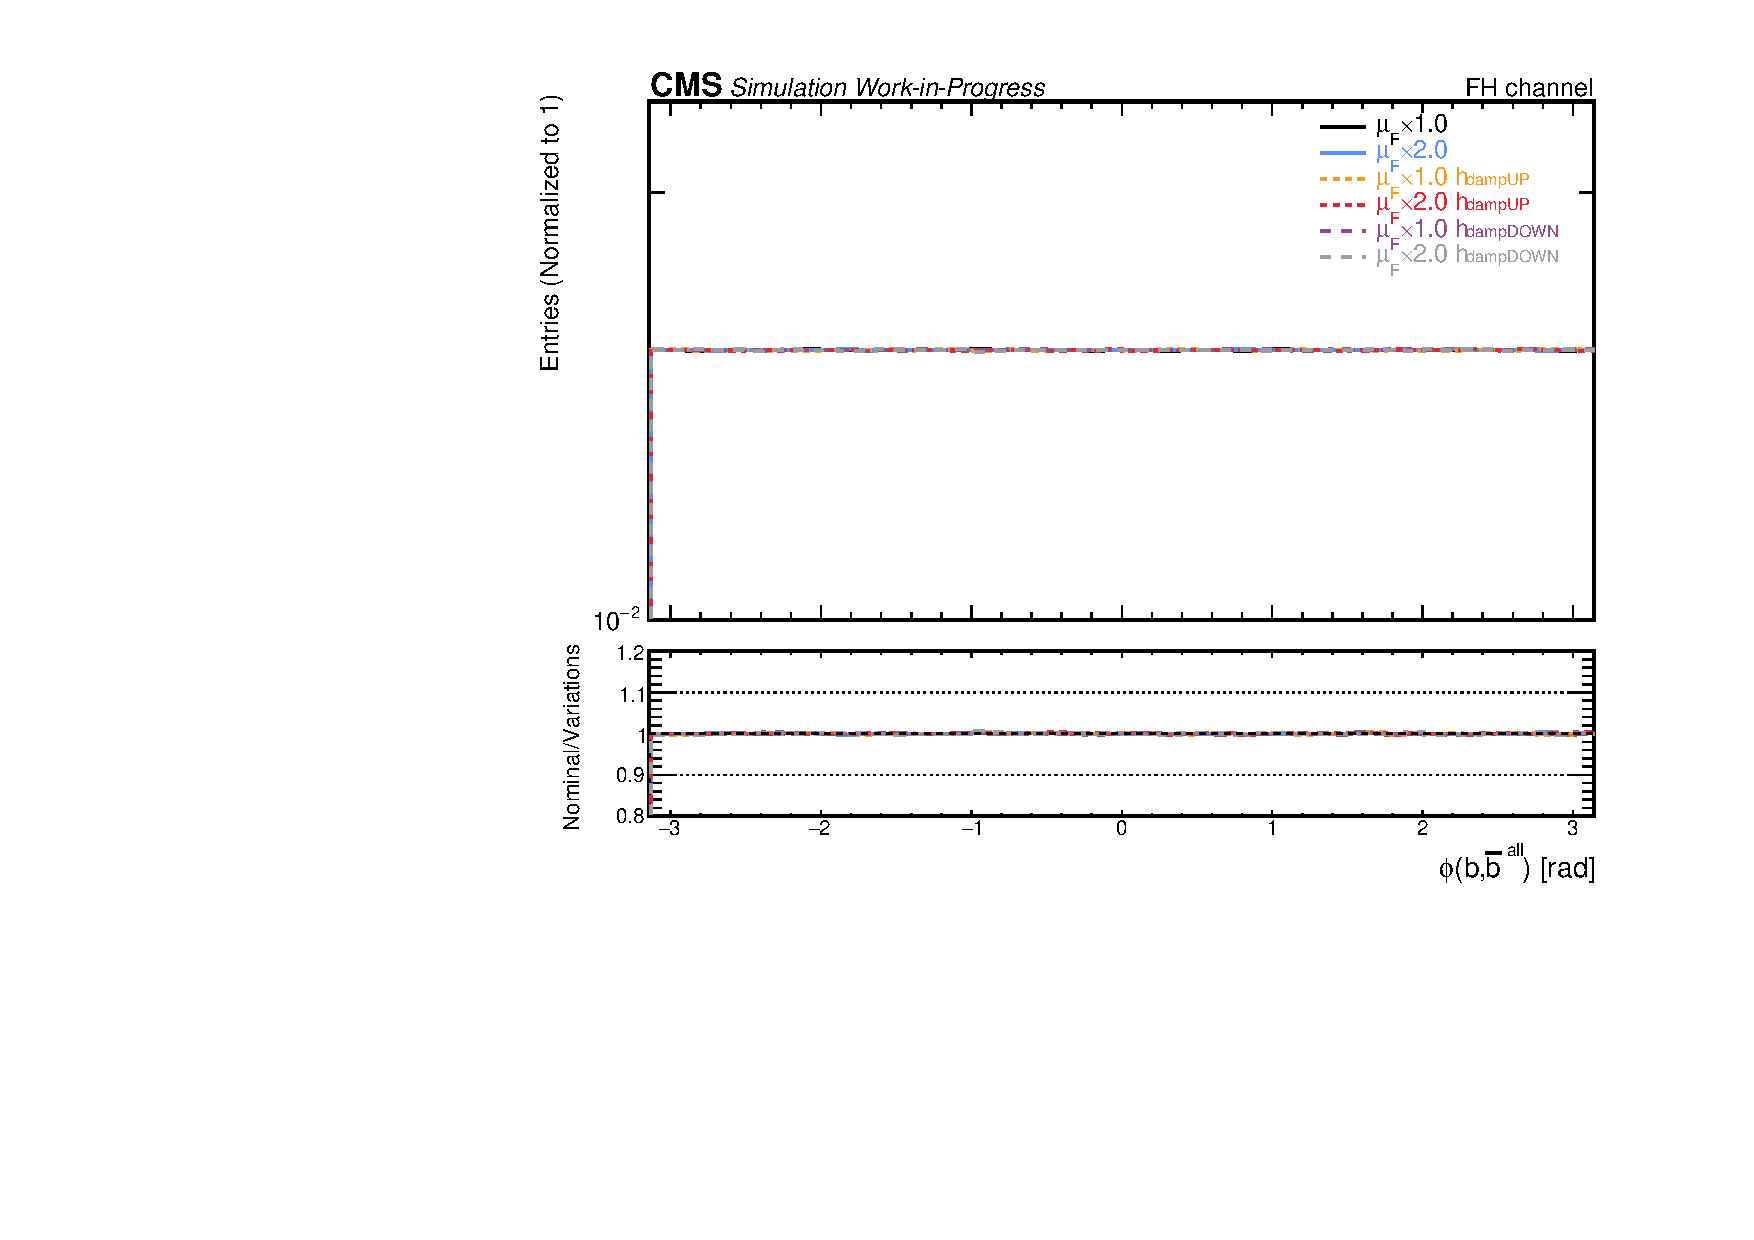
\includegraphics[width= 1.1\linewidth]{DL/ratio_b_all_phi.pdf}
        \caption{}
        \label{app:subfig:phi(b_all)_DL}
    \end{subfigure}
    \begin{subfigure}{0.49\textwidth}
        \centering
        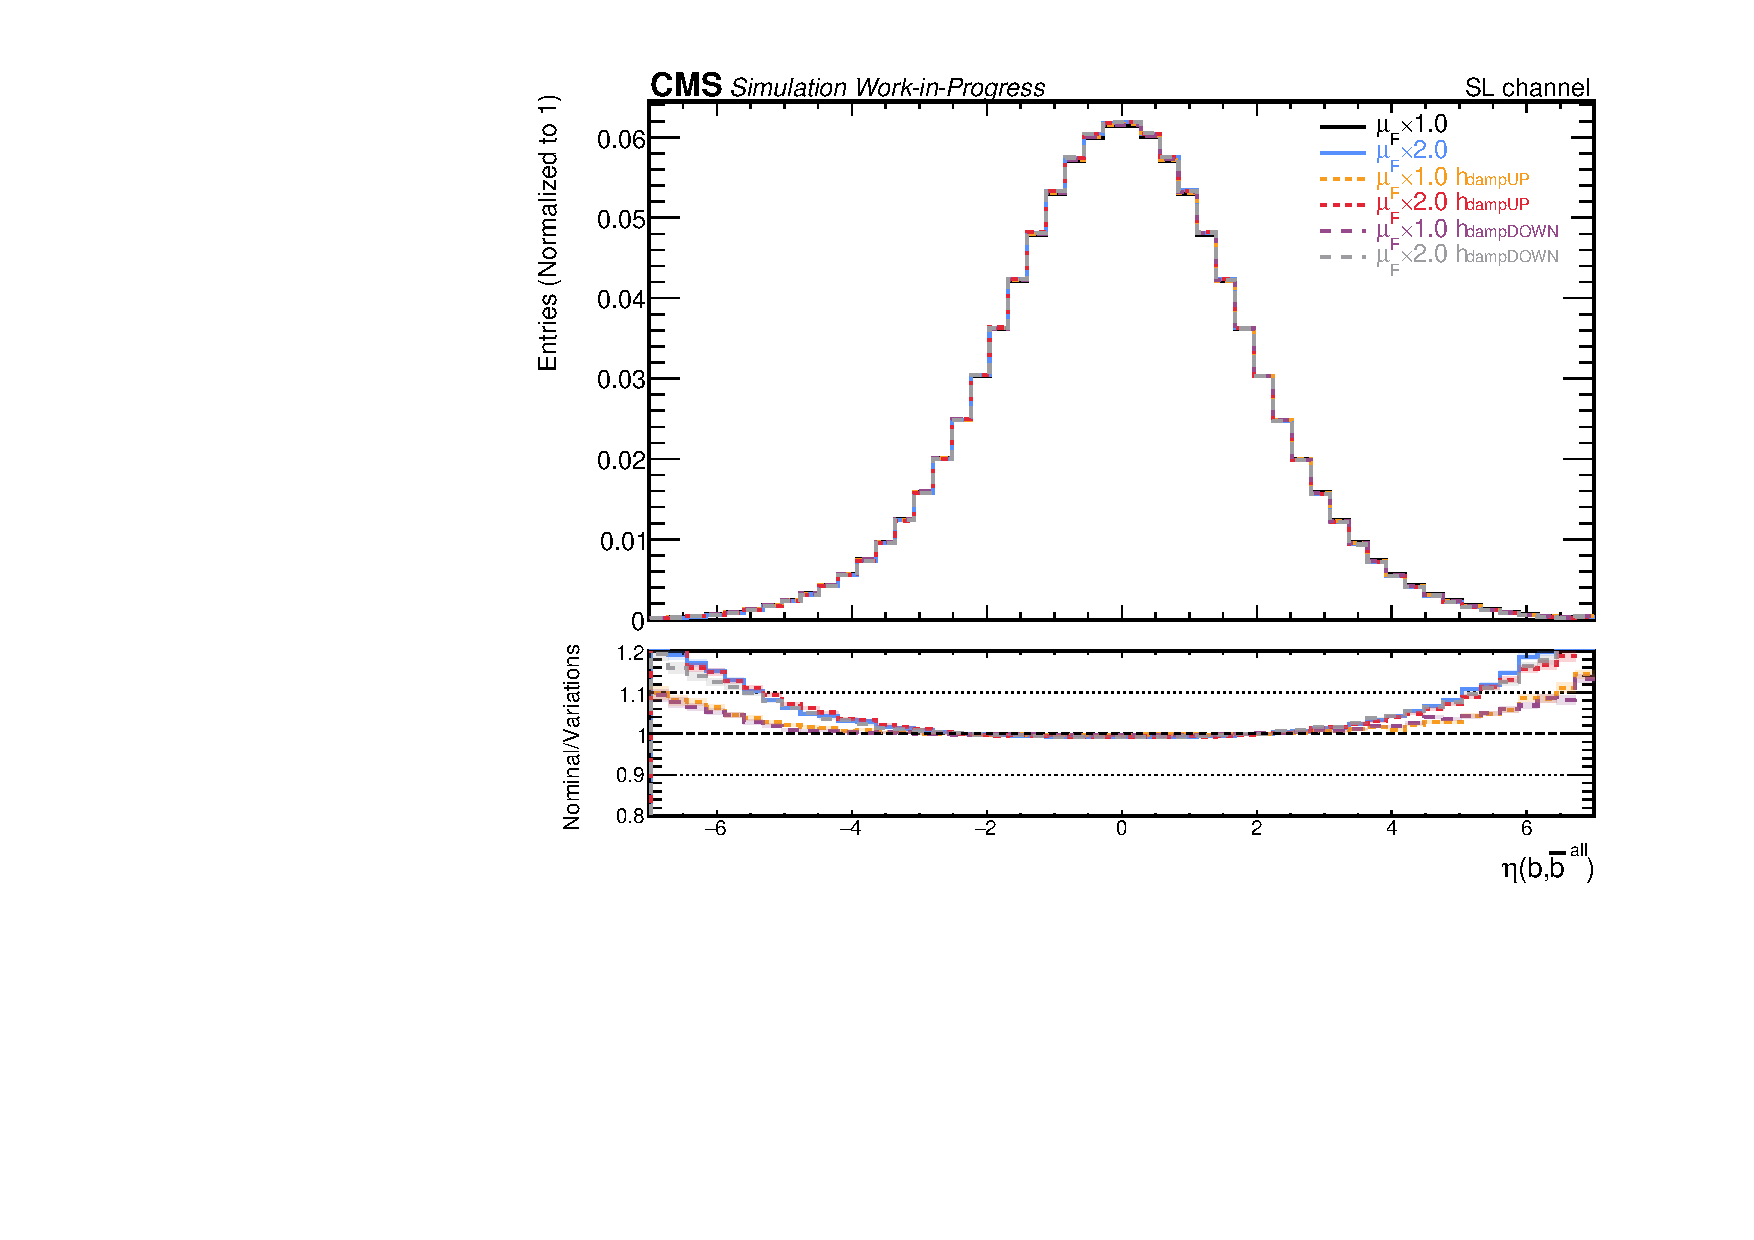
\includegraphics[width= 1.1\linewidth]{DL/ratio_b_all_pseudorapidity.pdf}
        \caption{}
        \label{app:subfig:eta(b_all)_DL}
    \end{subfigure}
    \caption{Distributions of (a) energy, (b) transverse momentum,  (c) azimuthal angle and (d) pseudorapidity of all the b/$\overline{\text{b}}$ quarks for the six different settings used in the simulation. The lower panel shows the ratio of the nominal setting to the variations. The shaded bands represent statistical uncertainties. The last bins contain the overflow events.}
    \label{app:fig:b_all_DL}
\end{figure}



\begin{figure}[H]
    \centering
    \begin{subfigure}{0.49\textwidth}
        \centering
        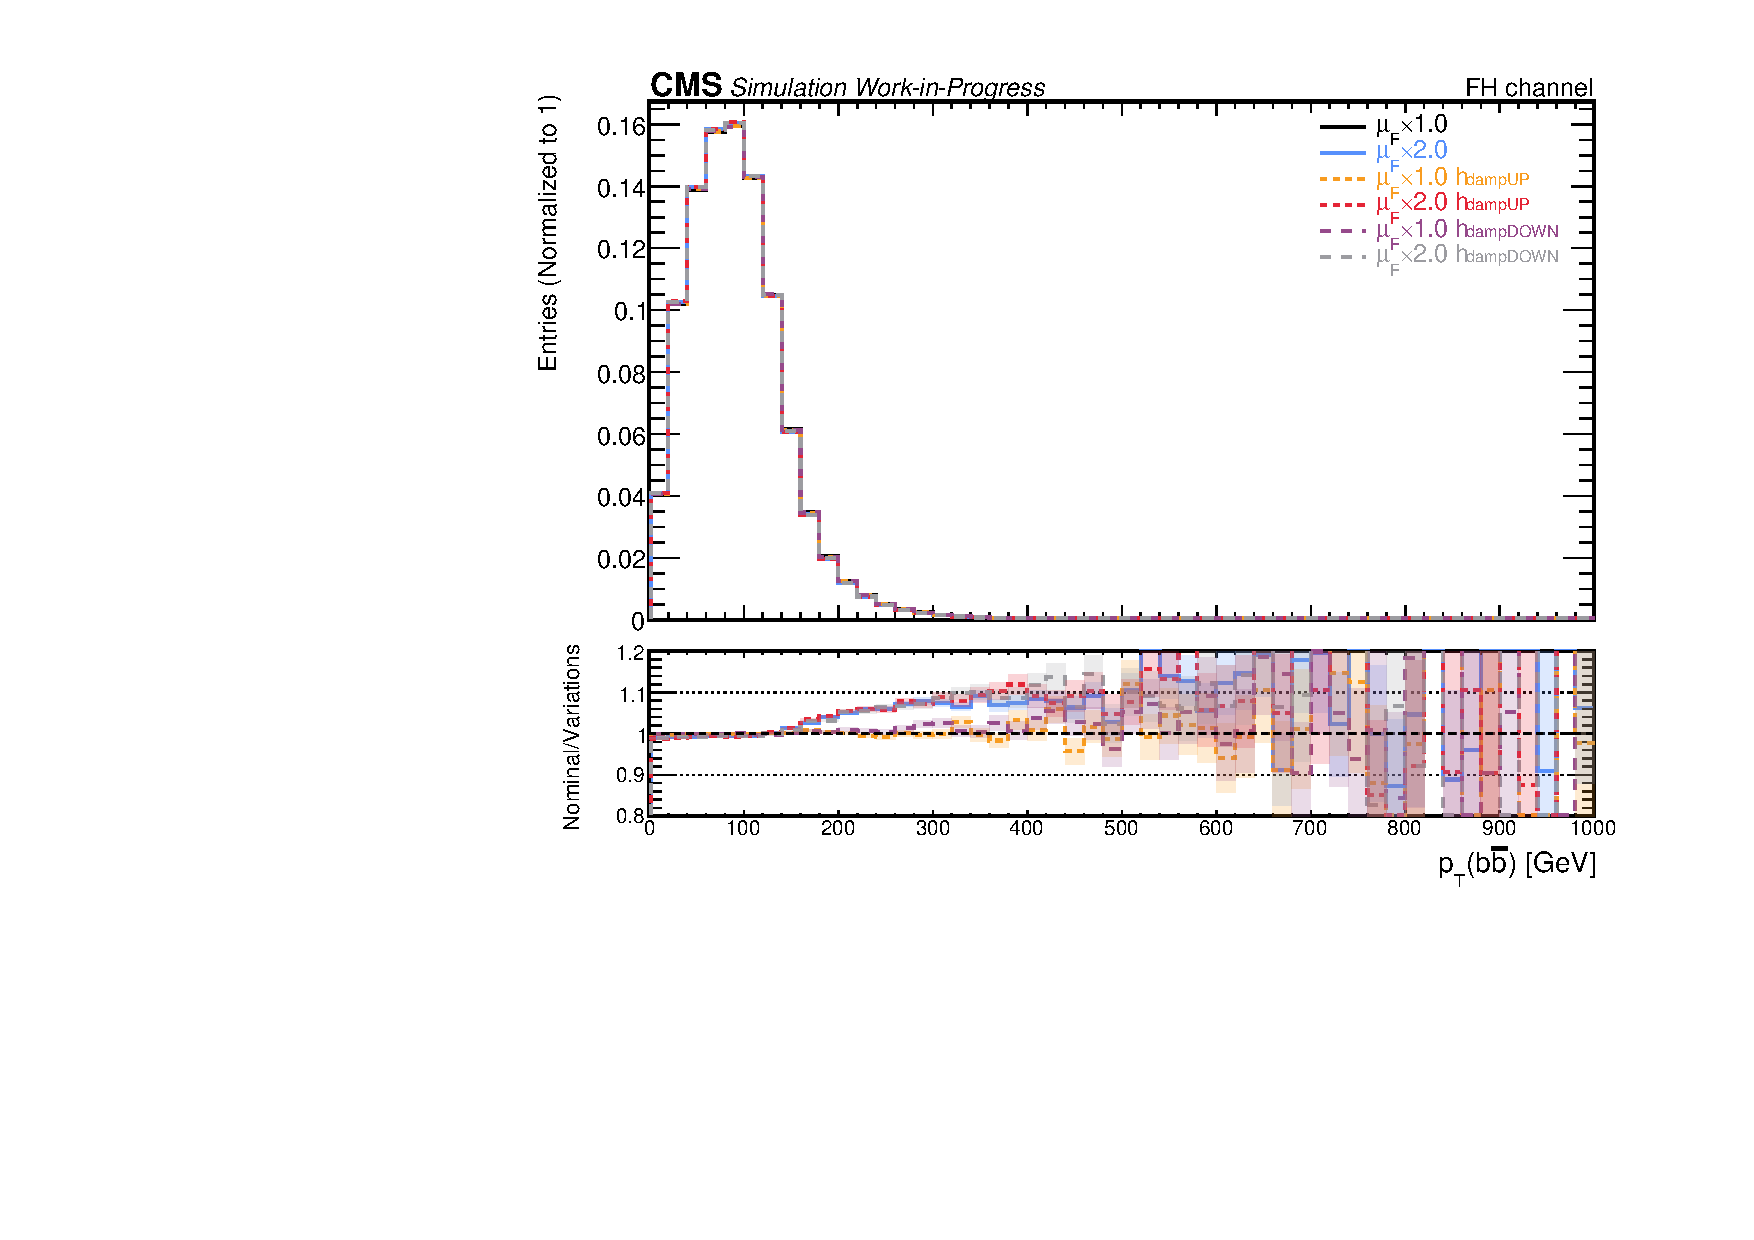
\includegraphics[width= 1.1\linewidth]{DL/ratio_bs_from_top_pt.pdf}
        \caption{}
        \label{app:subfig:pt(bbbar)_DL}
    \end{subfigure}
    \begin{subfigure}{0.49\textwidth}
        \centering
        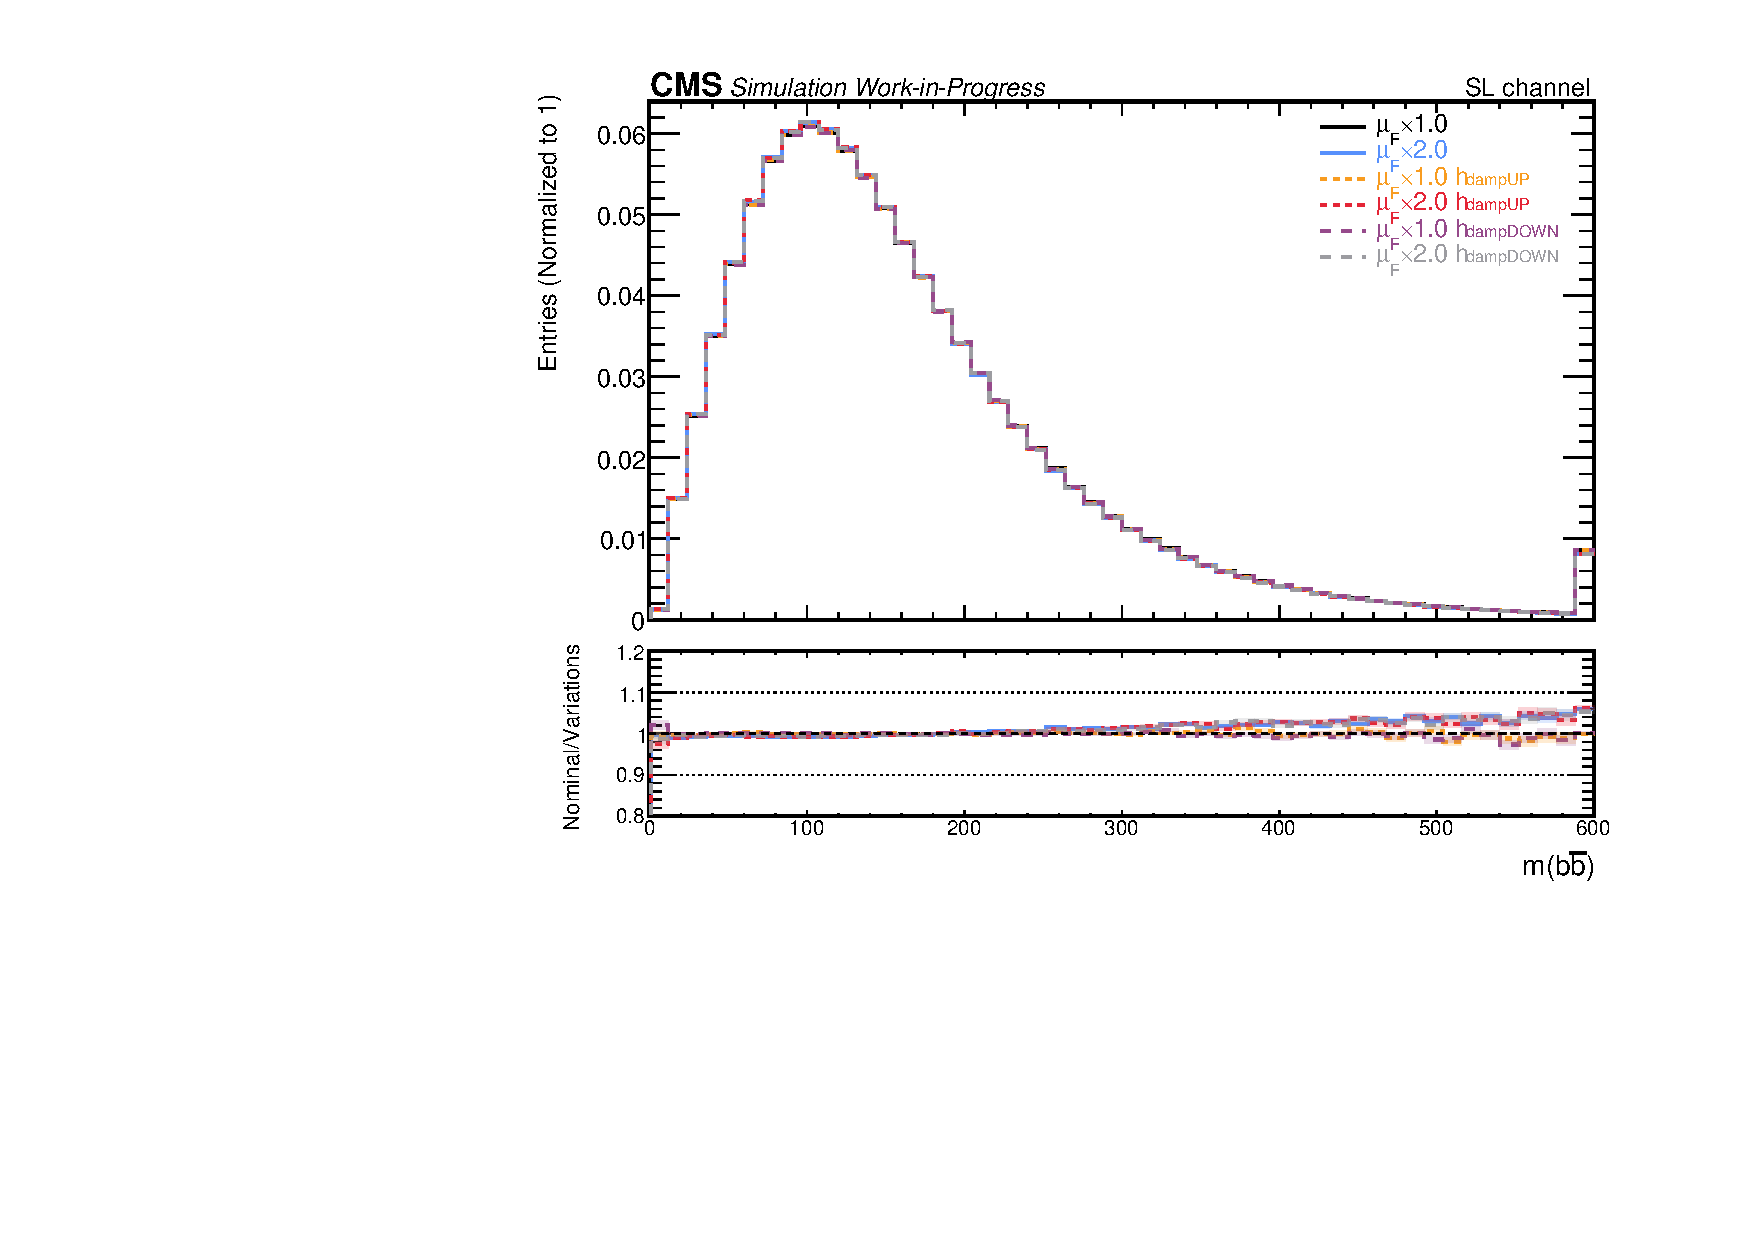
\includegraphics[width= 1.1\linewidth]{DL/ratio_bs_from_top_invariant_mass.pdf}
        \caption{}
        \label{app:subfig:m(bbbar)_DL}
    \end{subfigure}

    \vspace{0.2cm}
    
    \begin{subfigure}{0.49\textwidth}
        \centering
        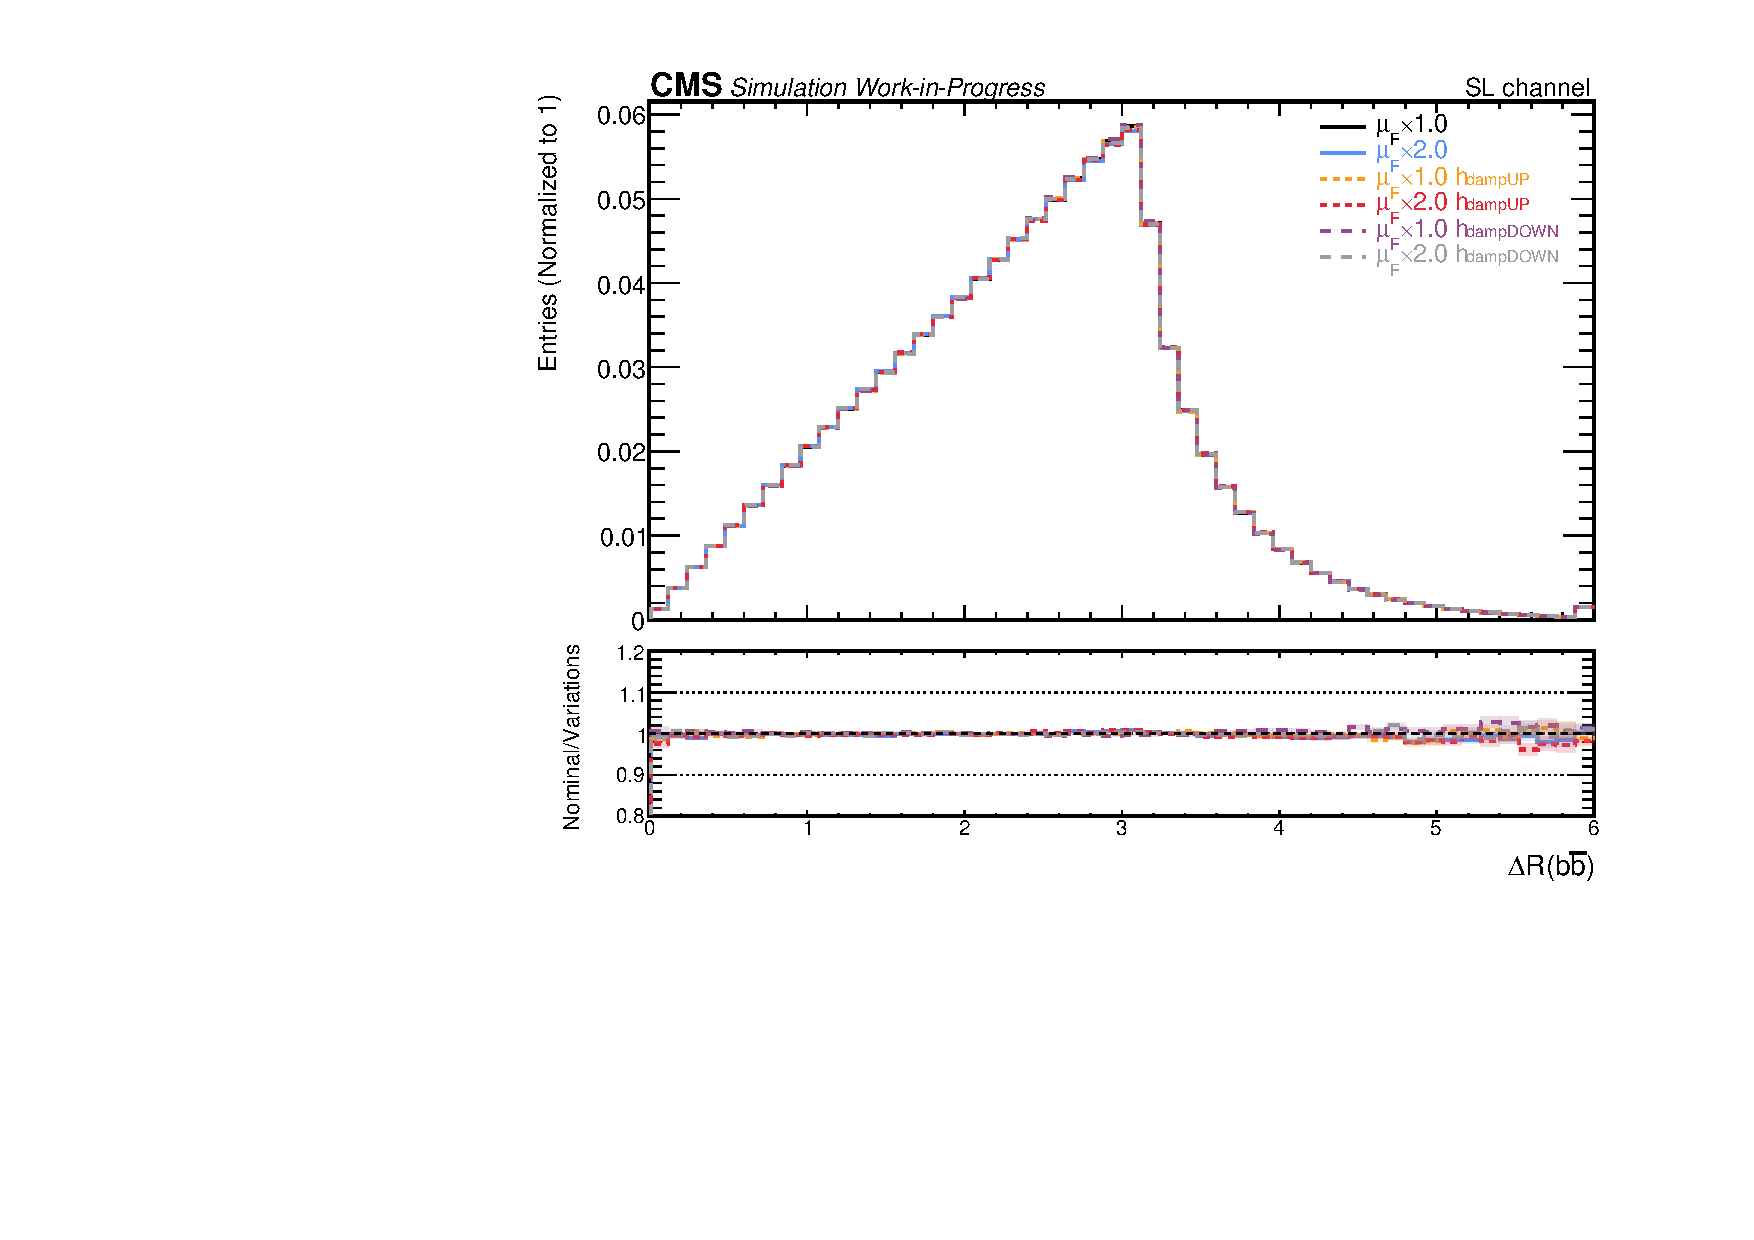
\includegraphics[width= 1.1\linewidth]{DL/ratio_bs_from_top_dR.pdf}
        \caption{}
        \label{app:subfig:dR(bbbar)_DL}
    \end{subfigure}
    \begin{subfigure}{0.49\textwidth}
        \centering
        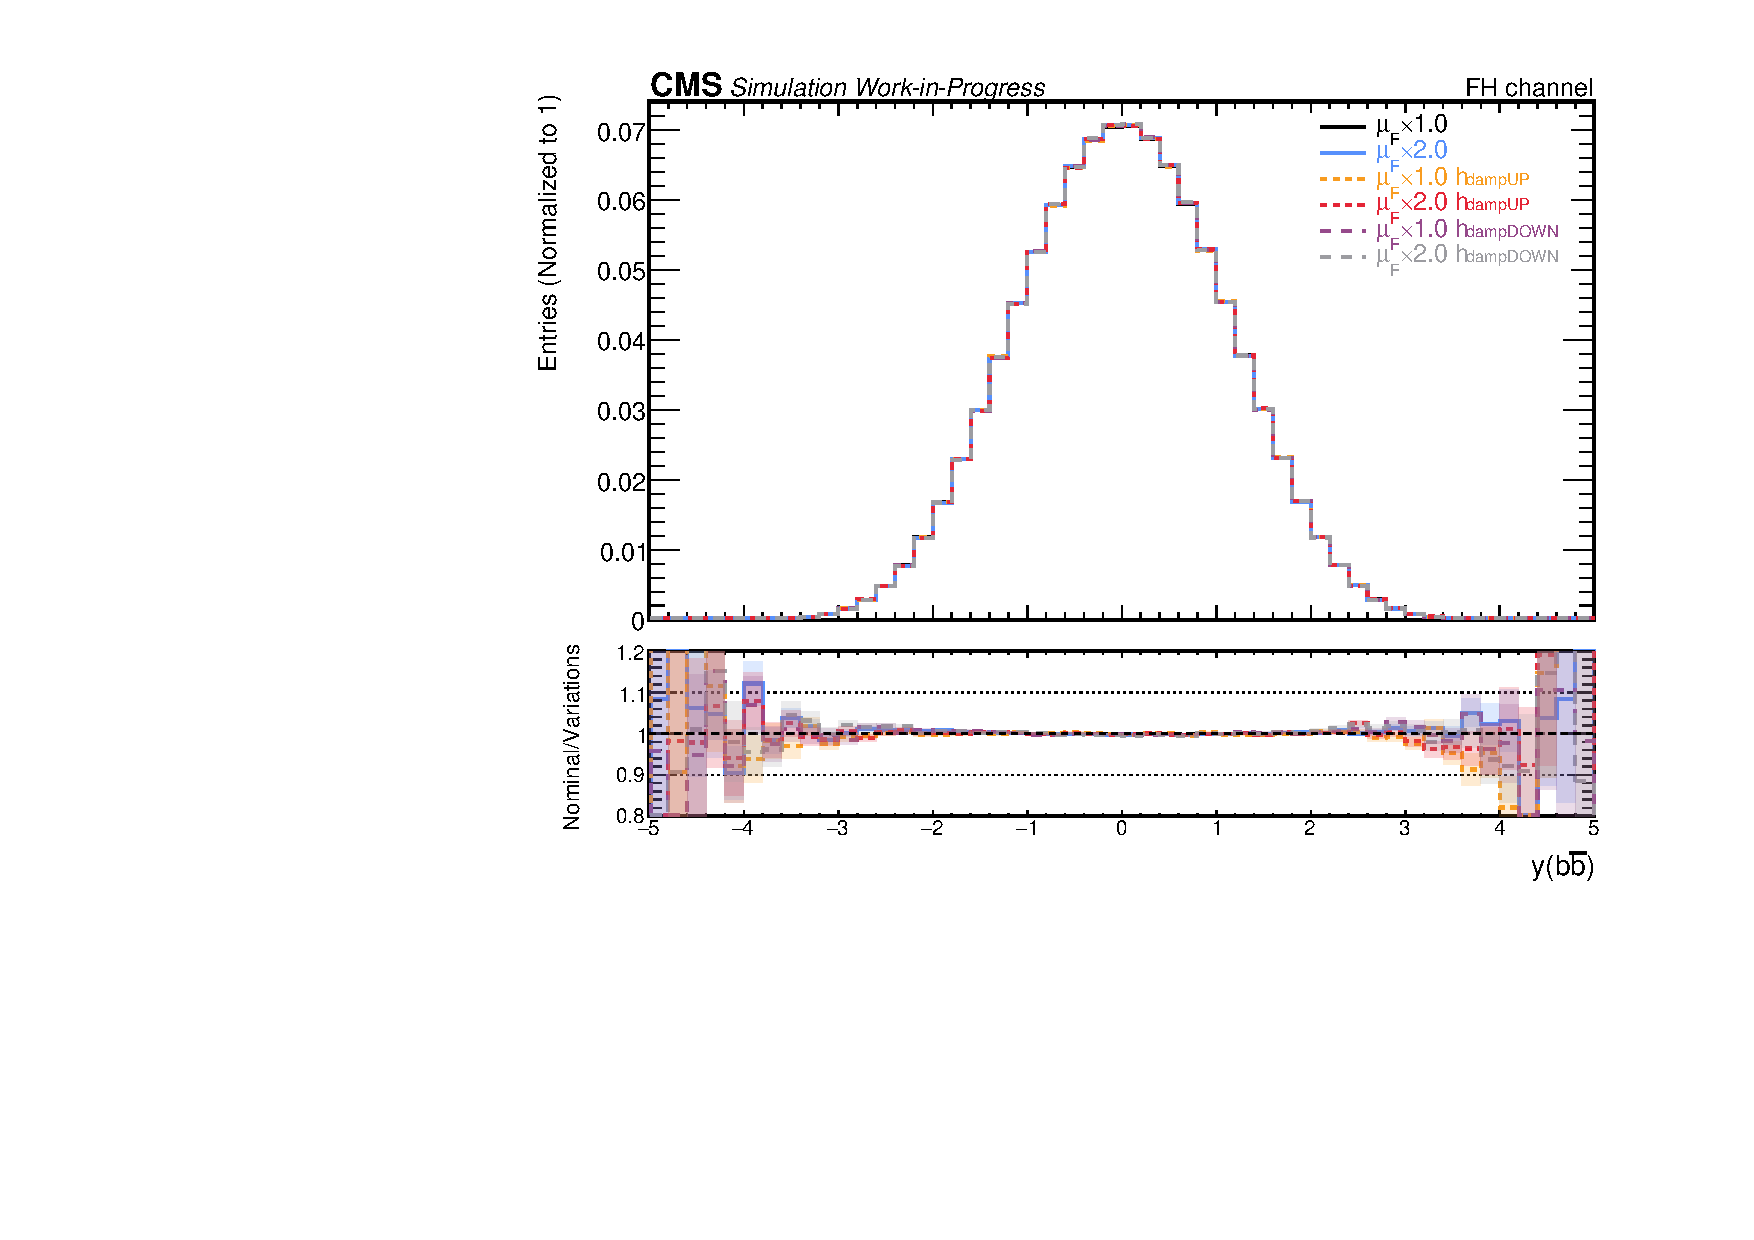
\includegraphics[width= 1.1\linewidth]{DL/ratio_bs_from_top_rapidity.pdf}
        \caption{}
        \label{app:subfig:y(bbbar)_DL}
    \end{subfigure}
    \caption{Distributions of (a) transverse momentum, (b) invariant mass,  (c) angular separation and (d) rapidity of the b$\overline{\text{b}}$ system, related to top quarks, for the six different settings used in the simulation. The lower panel shows the ratio of the nominal setting to the variations. The shaded bands represent statistical uncertainties. The last bins contain the overflow events.}
    \label{app:fig:bbbar_DL}
\end{figure}

\begin{figure}[H]
    \centering
    \begin{subfigure}{0.49\textwidth}
        \centering
        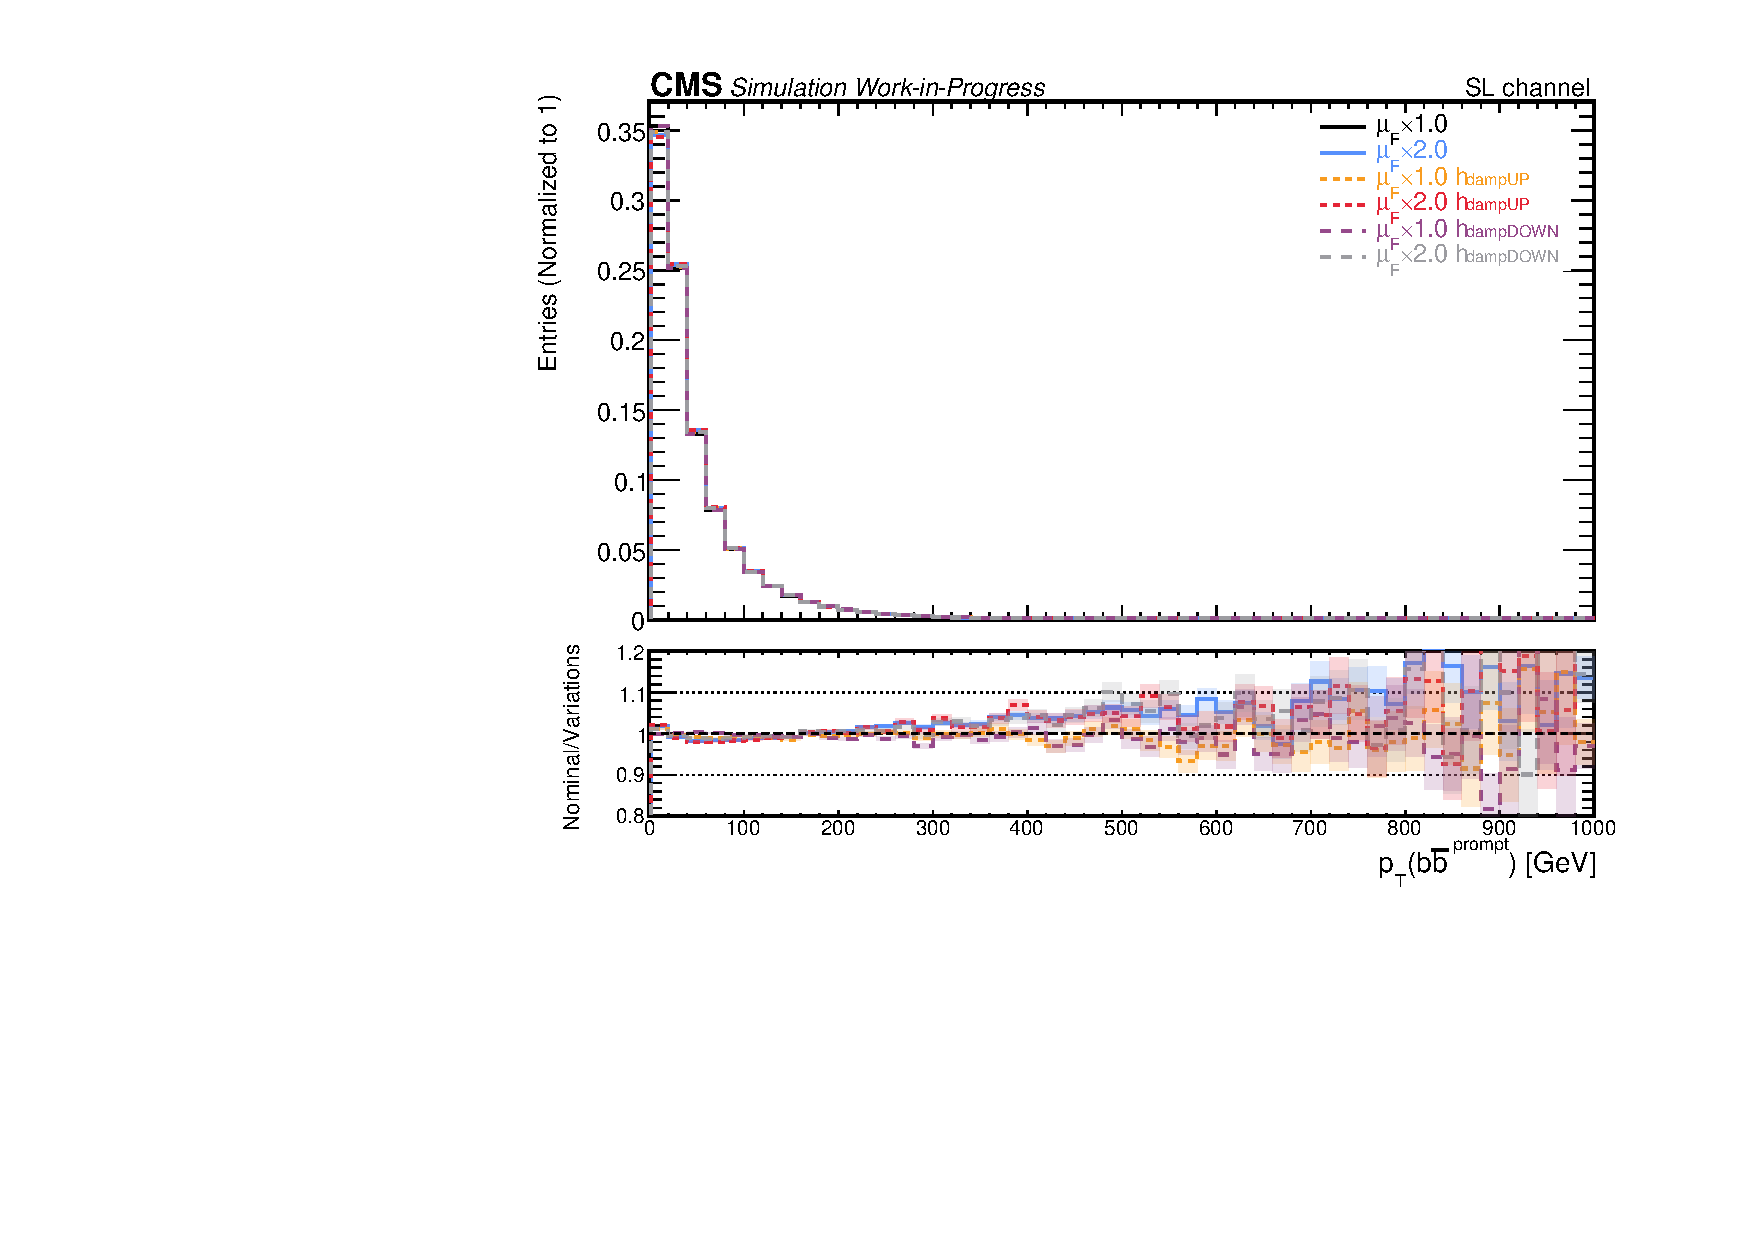
\includegraphics[width= 1.1\linewidth]{DL/ratio_prompt_bs_pt.pdf}
        \caption{}
        \label{app:subfig:pt(bbbar_prompt)_DL}
    \end{subfigure}
    \begin{subfigure}{0.49\textwidth}
        \centering
        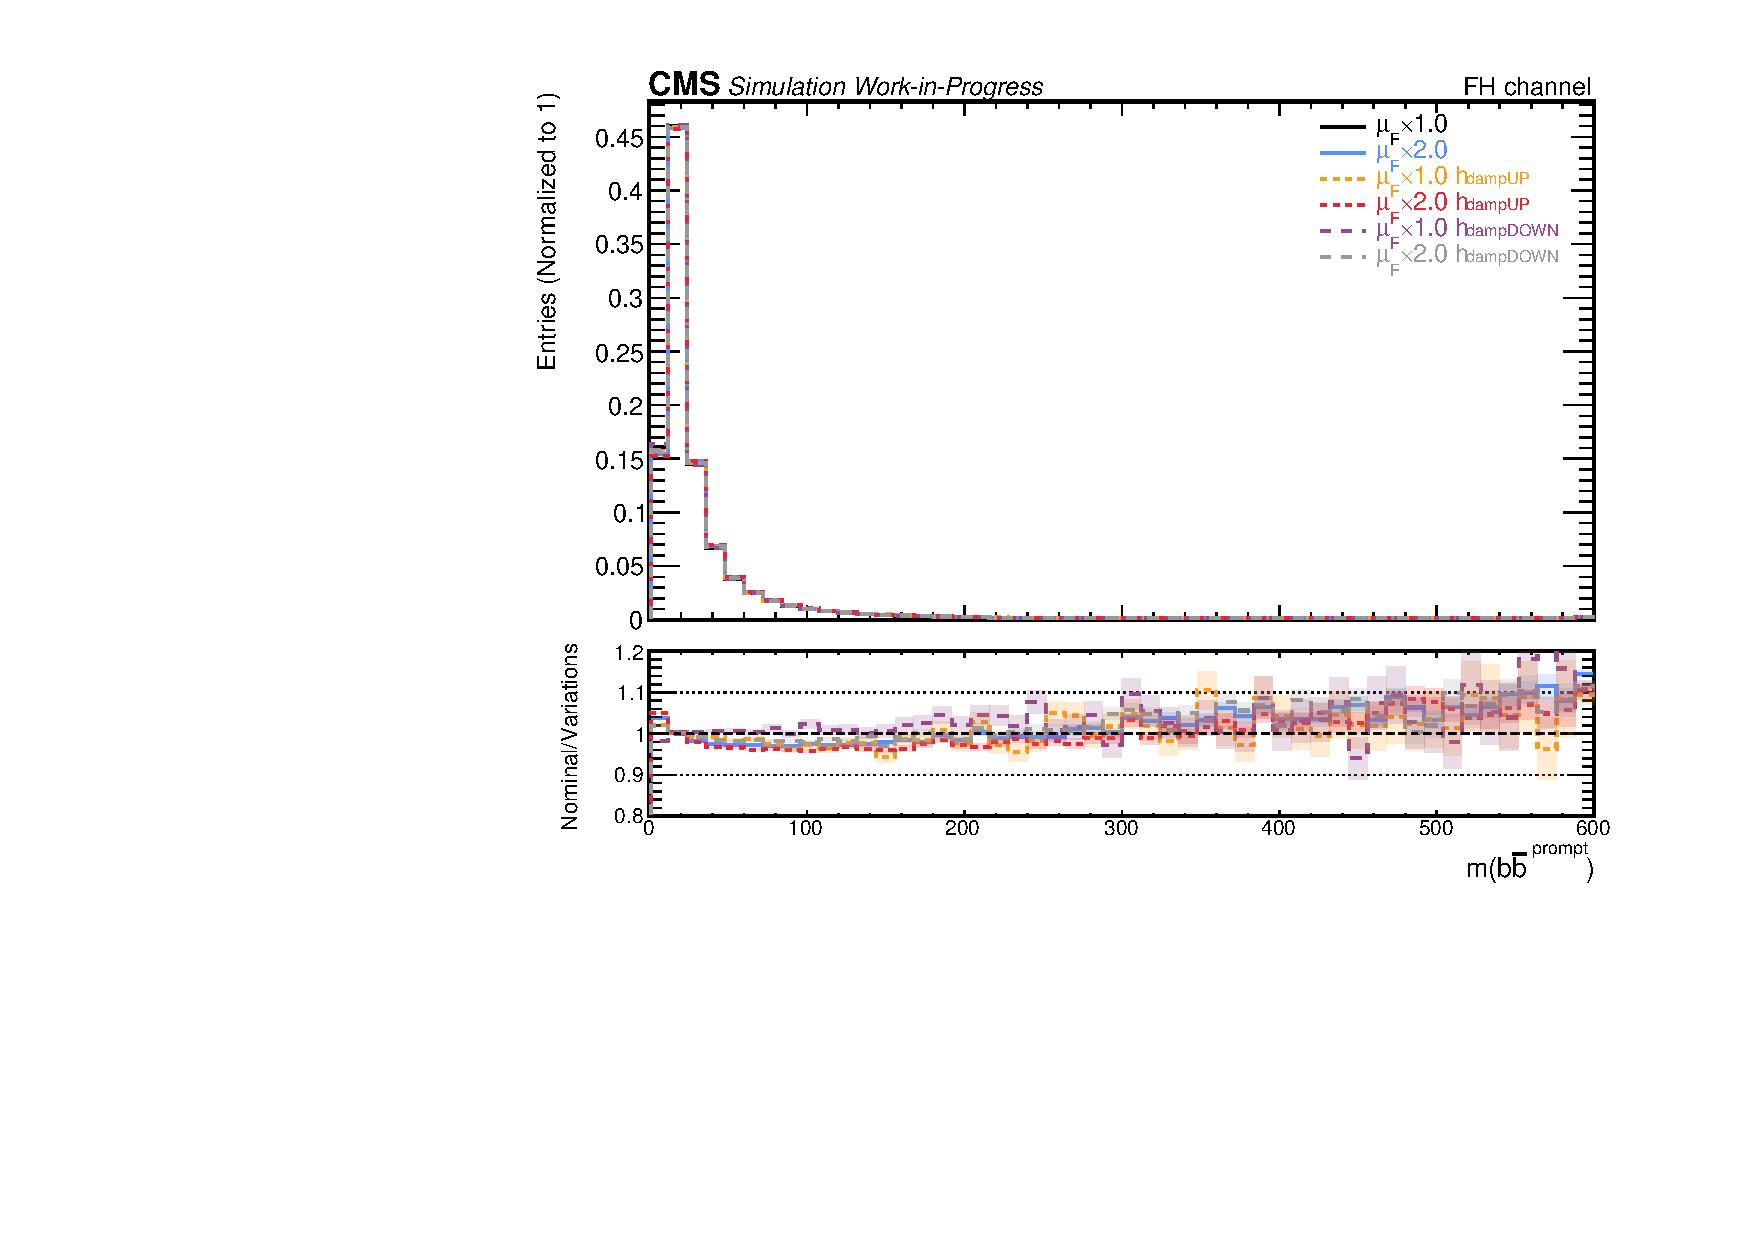
\includegraphics[width= 1.1\linewidth]{DL/ratio_prompt_bs_invariant_mass.pdf}
        \caption{}
        \label{app:subfig:m(bbbar_prompt)_DL}
    \end{subfigure}

    \vspace{0.2cm}
    
    \begin{subfigure}{0.49\textwidth}
        \centering
        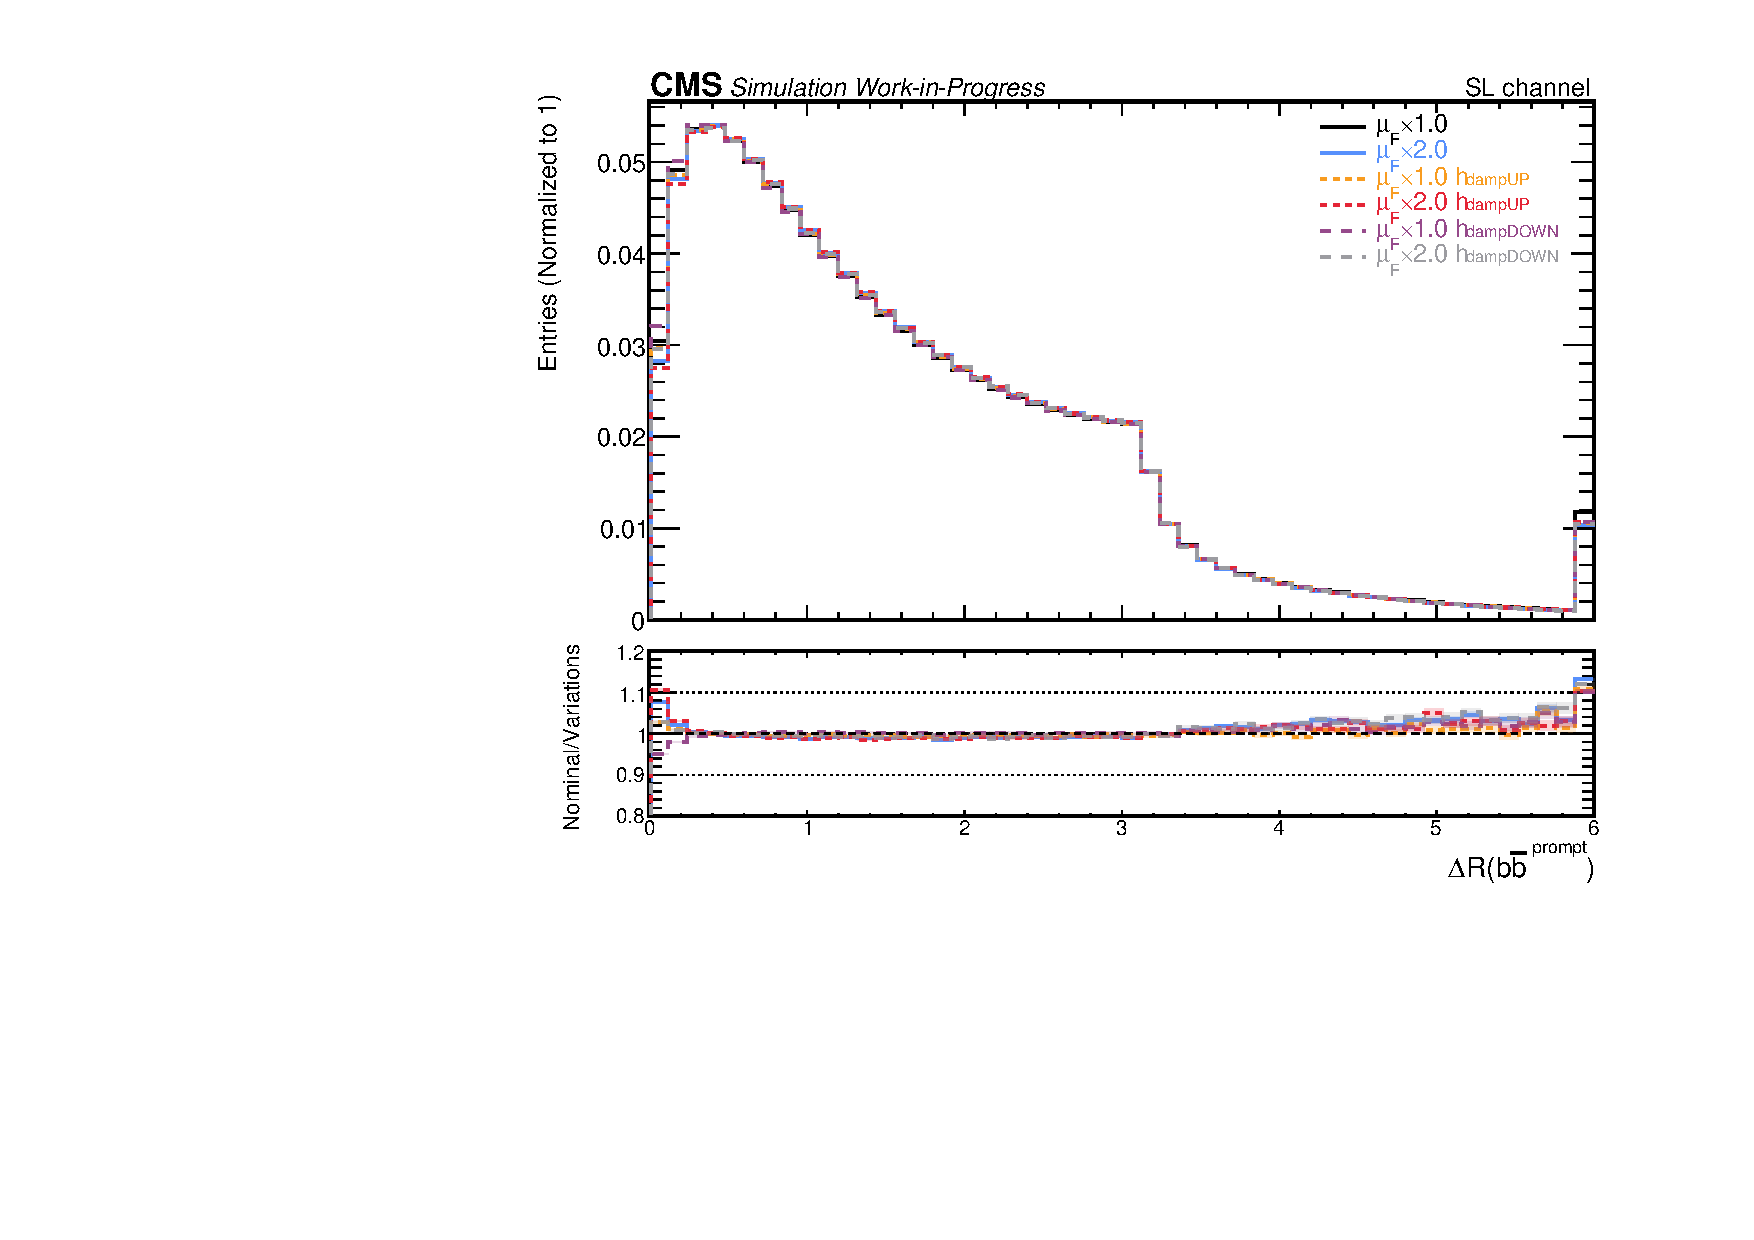
\includegraphics[width= 1.1\linewidth]{DL/ratio_prompt_bs_dR.pdf}
        \caption{}
        \label{app:subfig:dR(bbbar_prompt)_DL}
    \end{subfigure}
    \begin{subfigure}{0.49\textwidth}
        \centering
        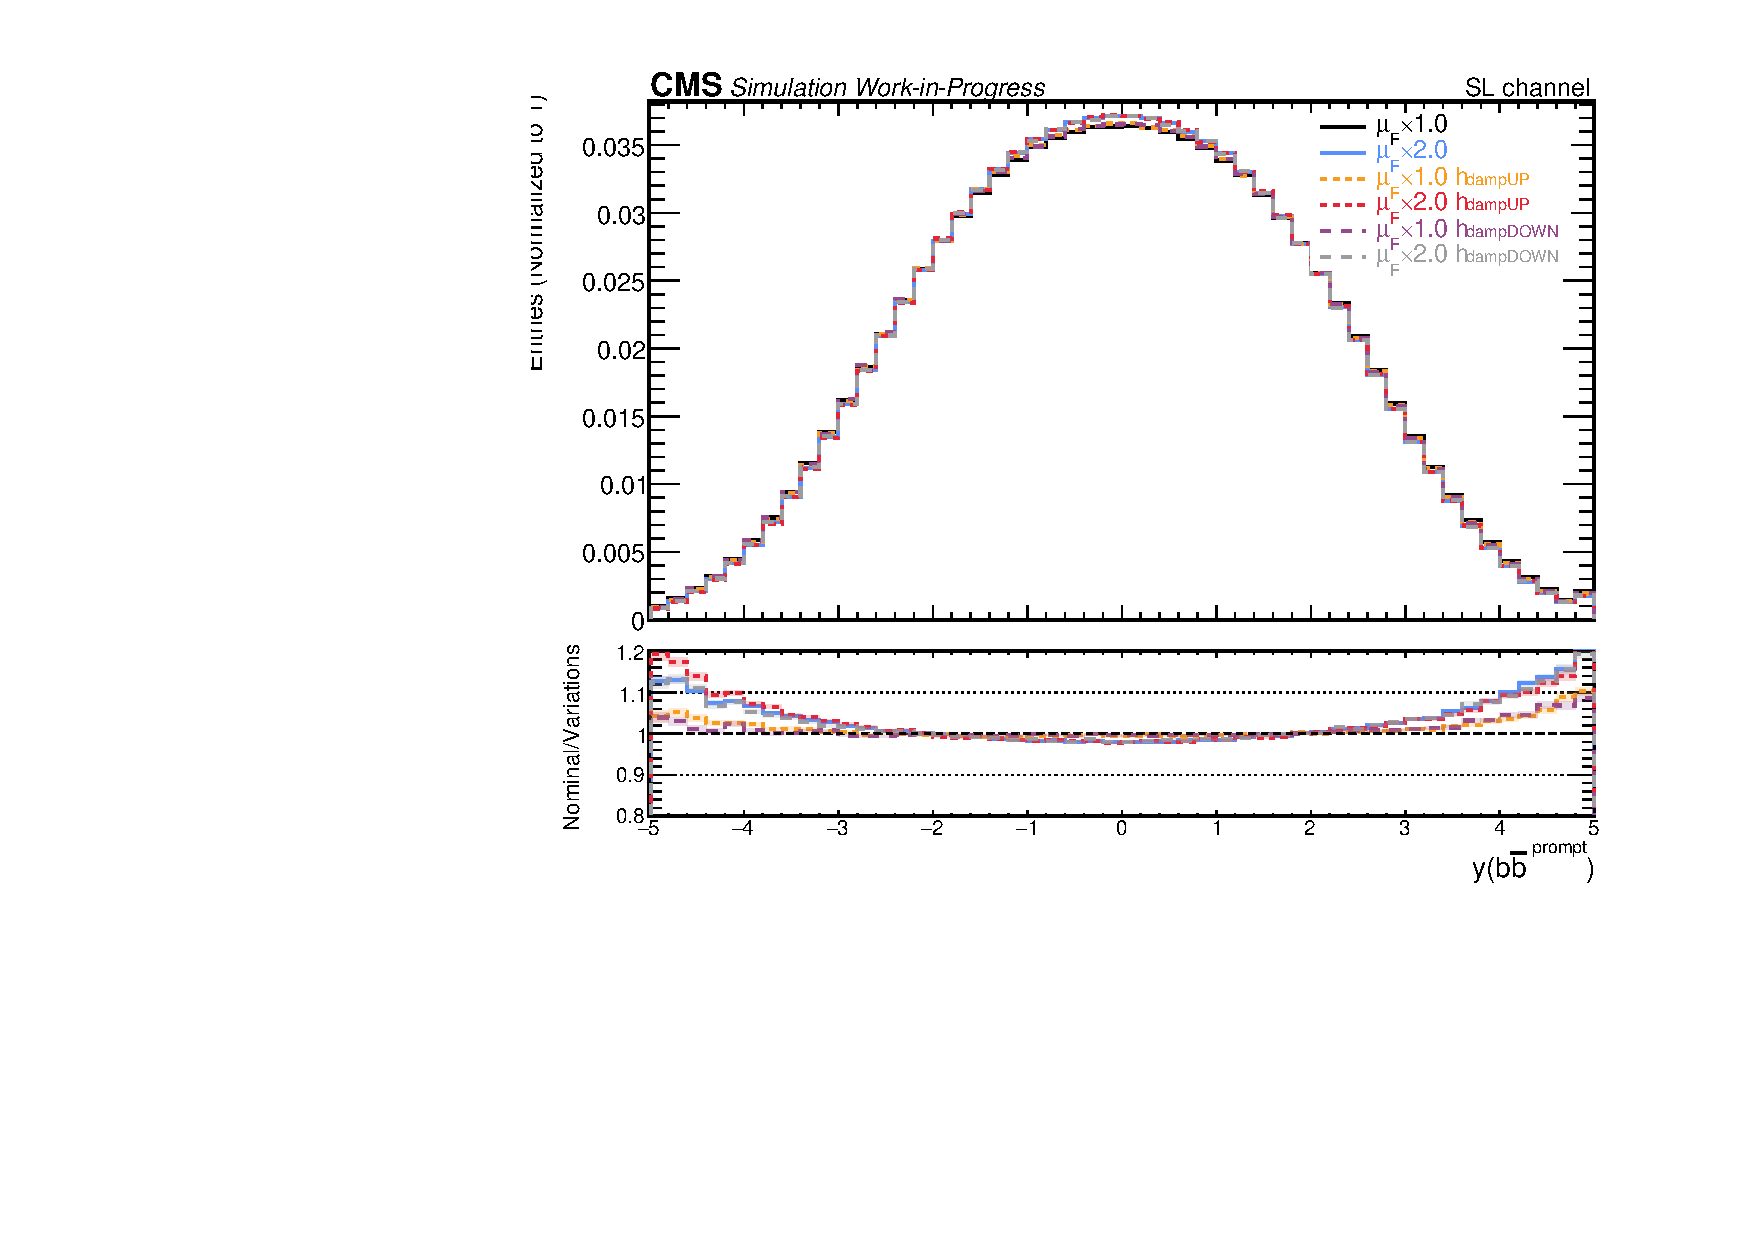
\includegraphics[width= 1.1\linewidth]{DL/ratio_prompt_bs_rapidity.pdf}
        \caption{}
        \label{app:subfig:y(bbbar_prompt)_DL}
    \end{subfigure}
    \caption{Distributions of (a) transverse momentum, (b) invariant mass,  (c) angular separation and (d) rapidity of the prompt b$\overline{\text{b}}$ system for the six different settings used in the simulation. The lower panel shows the ratio of the nominal setting to the variations. The shaded bands represent statistical uncertainties. The last bins contain the overflow events.}
    \label{app:fig:prompt_bbbar_DL}
\end{figure}


\begin{figure}[H]
    \centering
    \begin{subfigure}{0.49\textwidth}
        \centering
        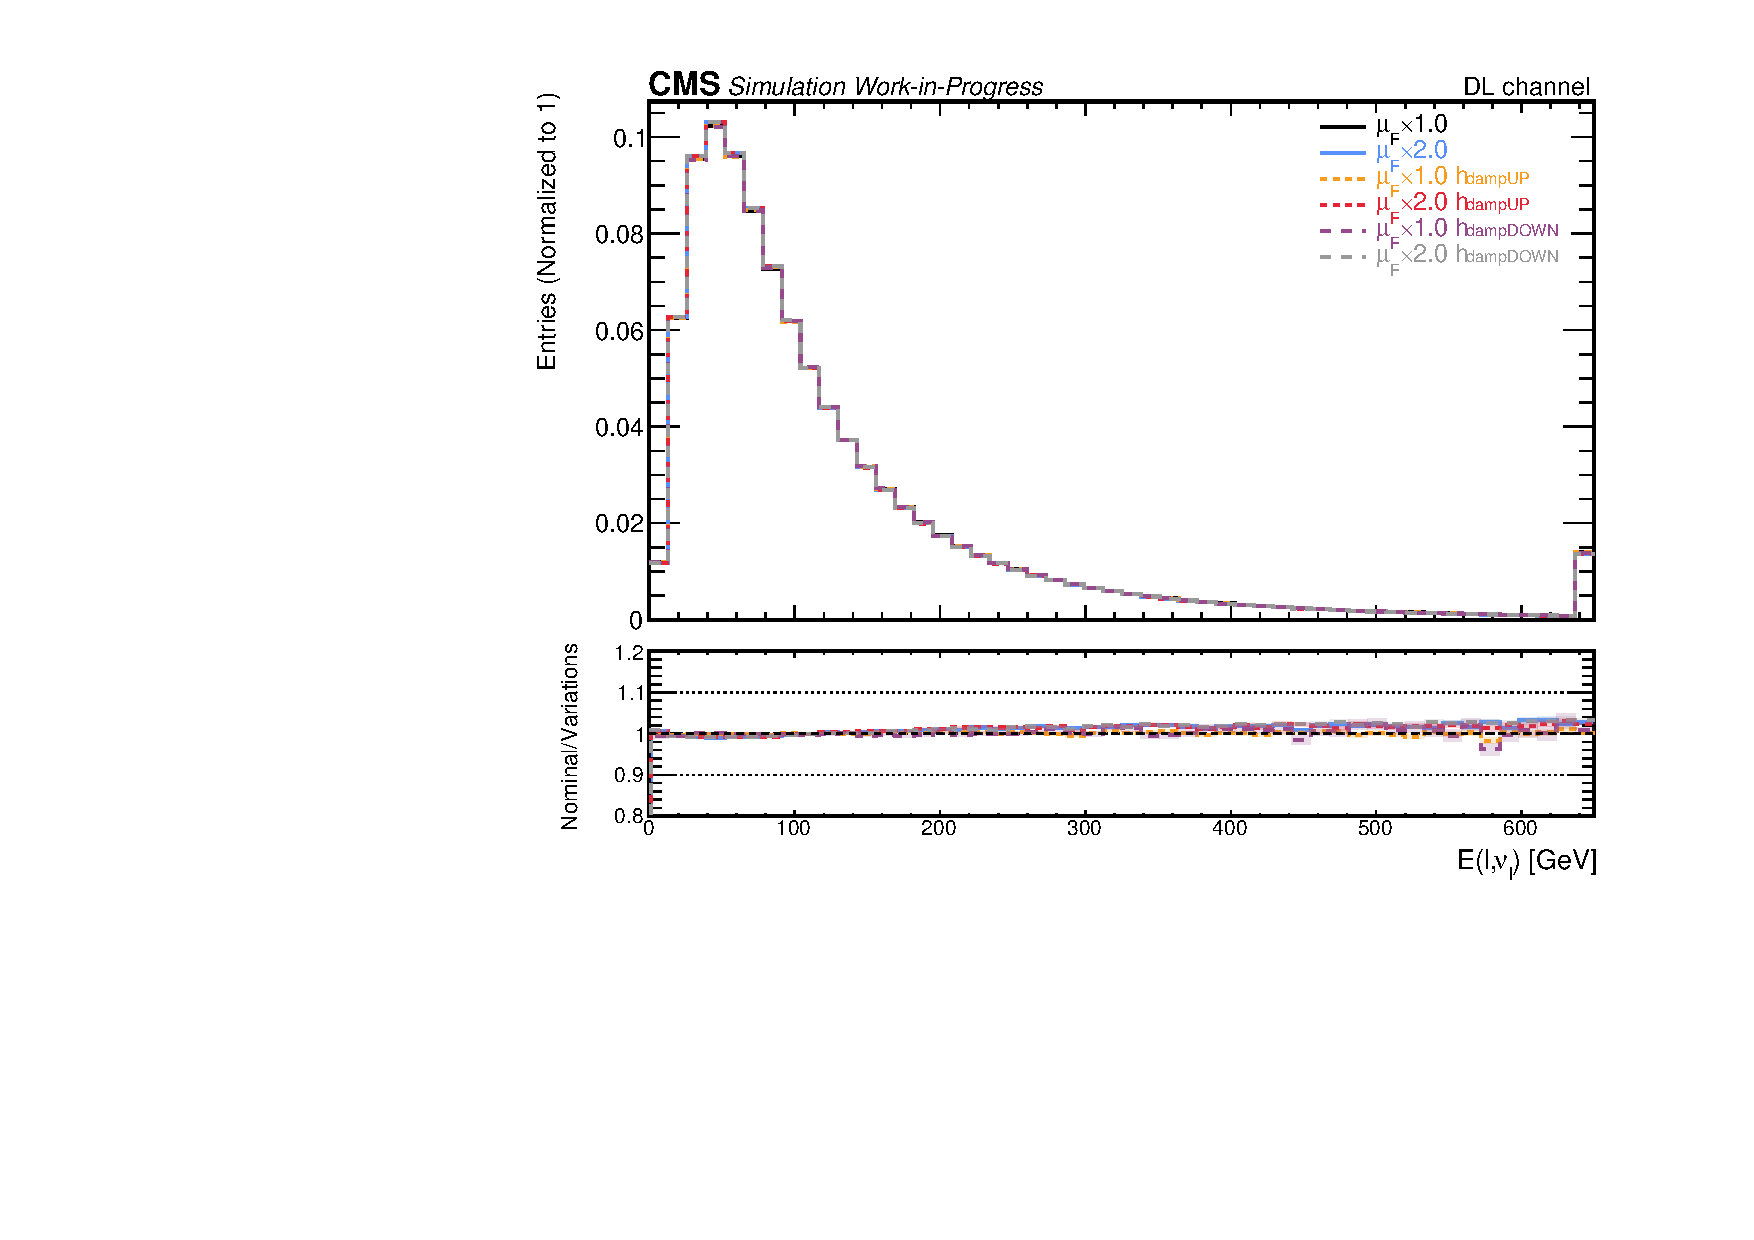
\includegraphics[width= 1.1\linewidth]{DL/ratio_leptons_energy.pdf}
        \caption{}
        \label{app:subfig:E(leptons)_DL}
    \end{subfigure}
    \begin{subfigure}{0.49\textwidth}
        \centering
        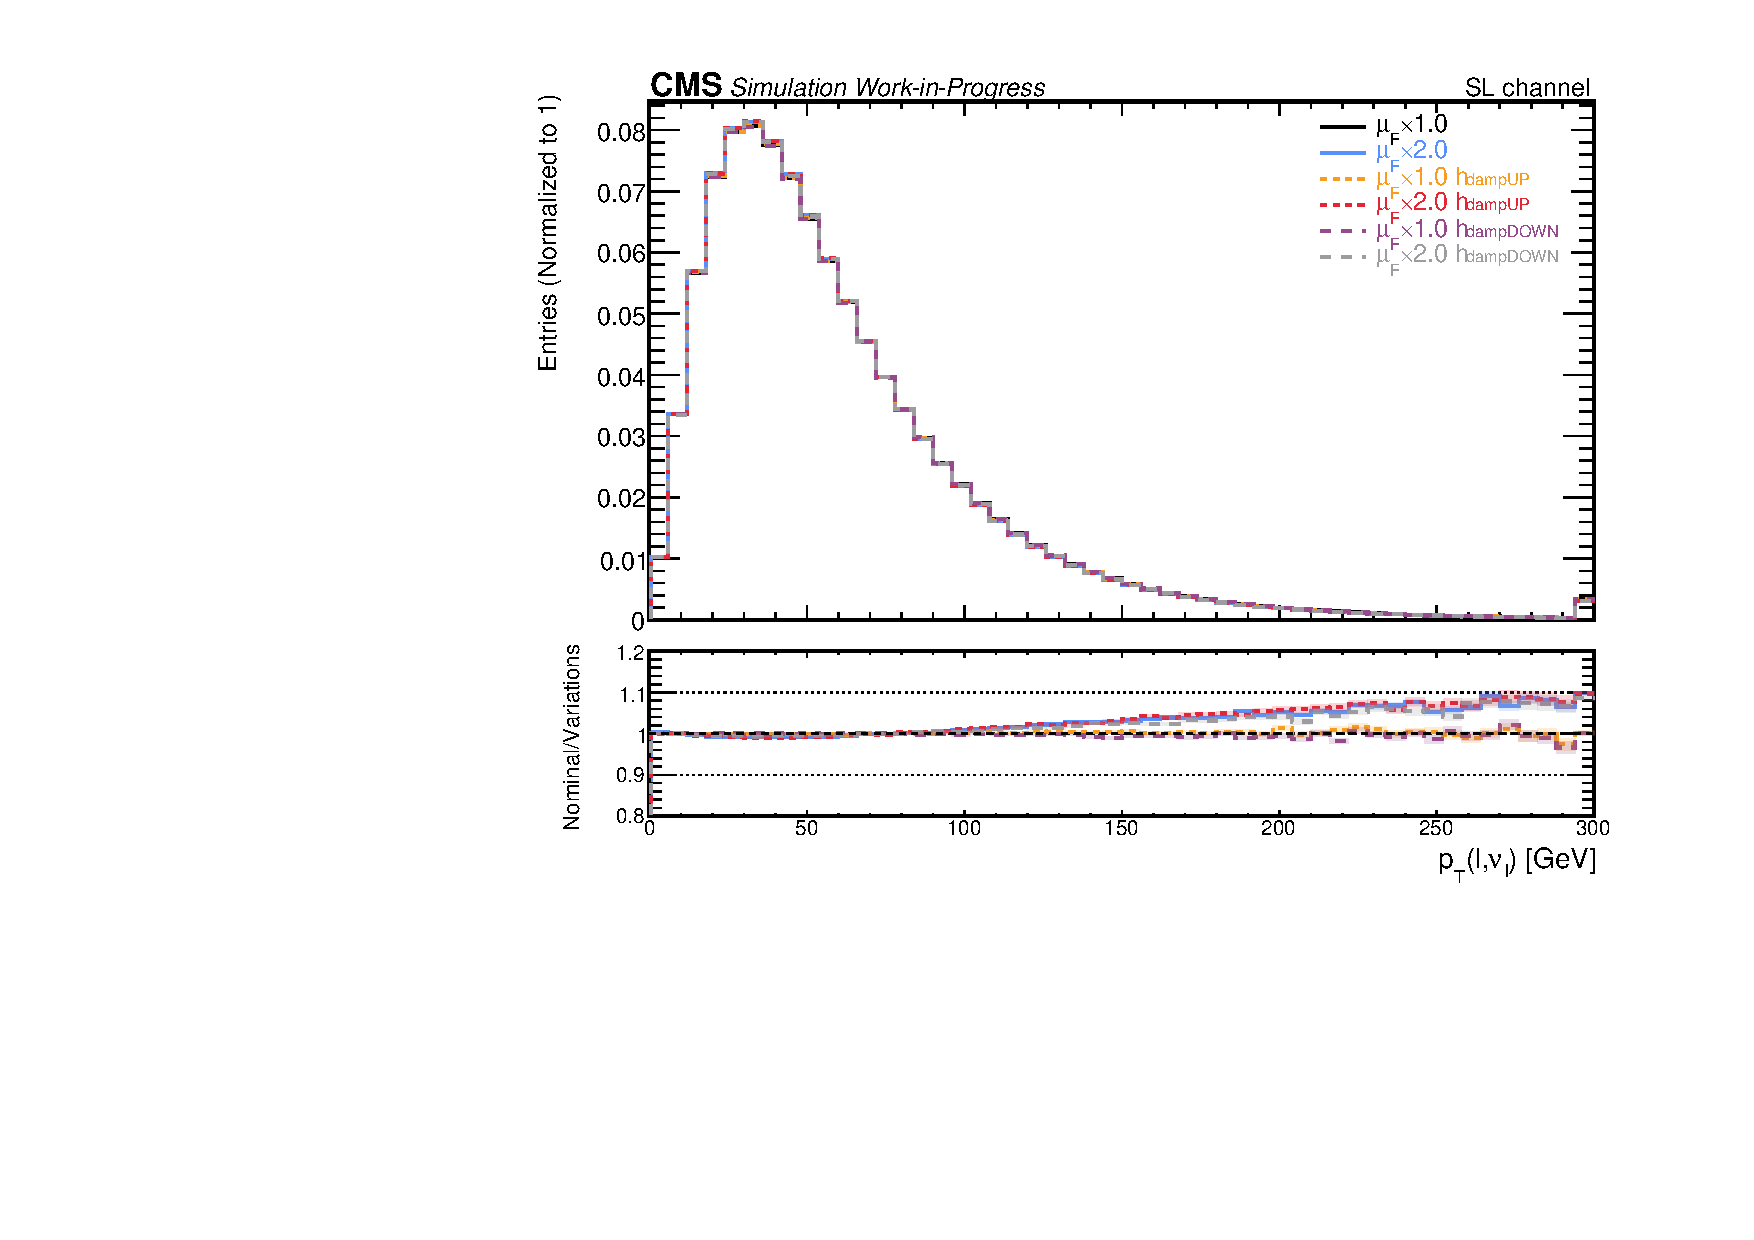
\includegraphics[width= 1.1\linewidth]{DL/ratio_leptons_pt.pdf}
        \caption{}
        \label{app:subfig:pt(leptons)_DL}
    \end{subfigure}

    \vspace{0.2cm}
    
    \begin{subfigure}{0.49\textwidth}
        \centering
        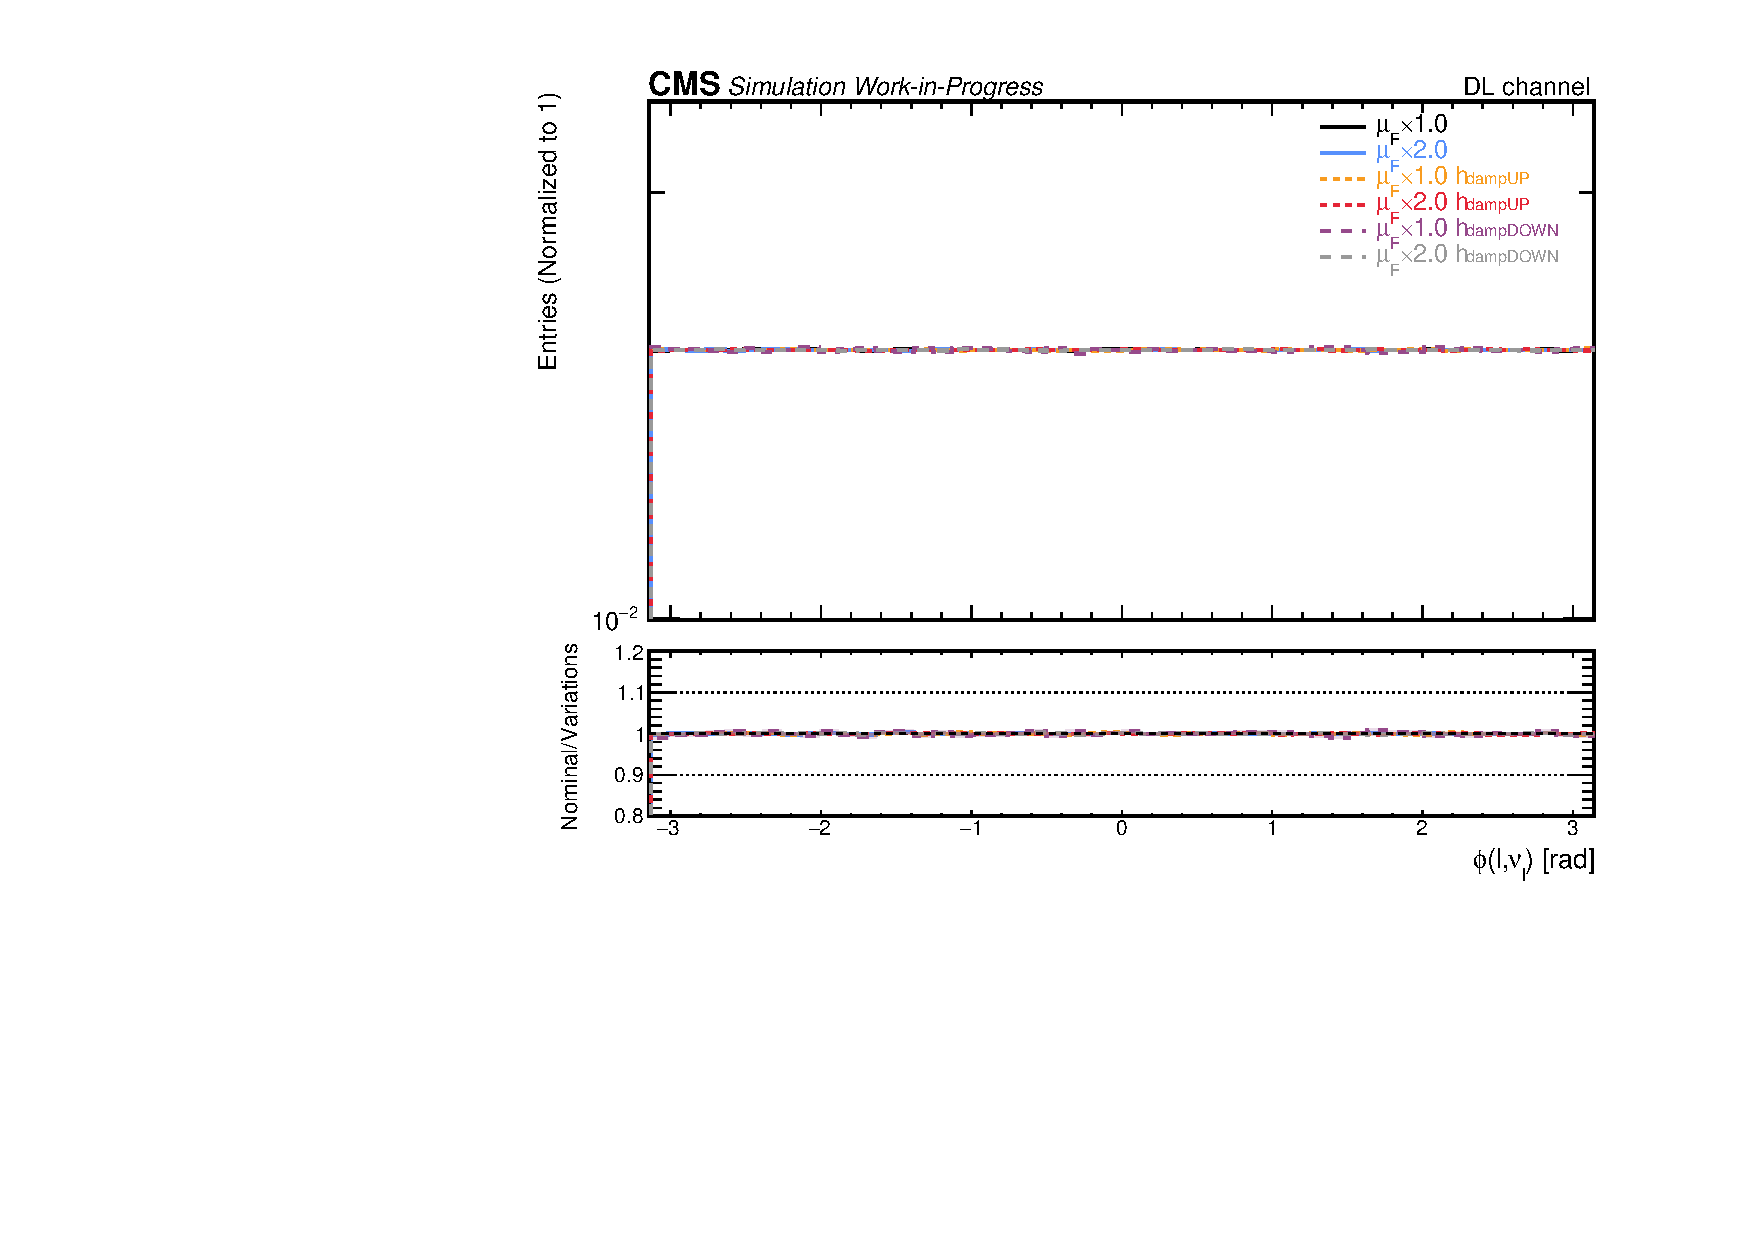
\includegraphics[width= 1.1\linewidth]{DL/ratio_leptons_phi.pdf}
        \caption{}
        \label{app:subfig:phi(leptons)_DL}
    \end{subfigure}
    \begin{subfigure}{0.49\textwidth}
        \centering
        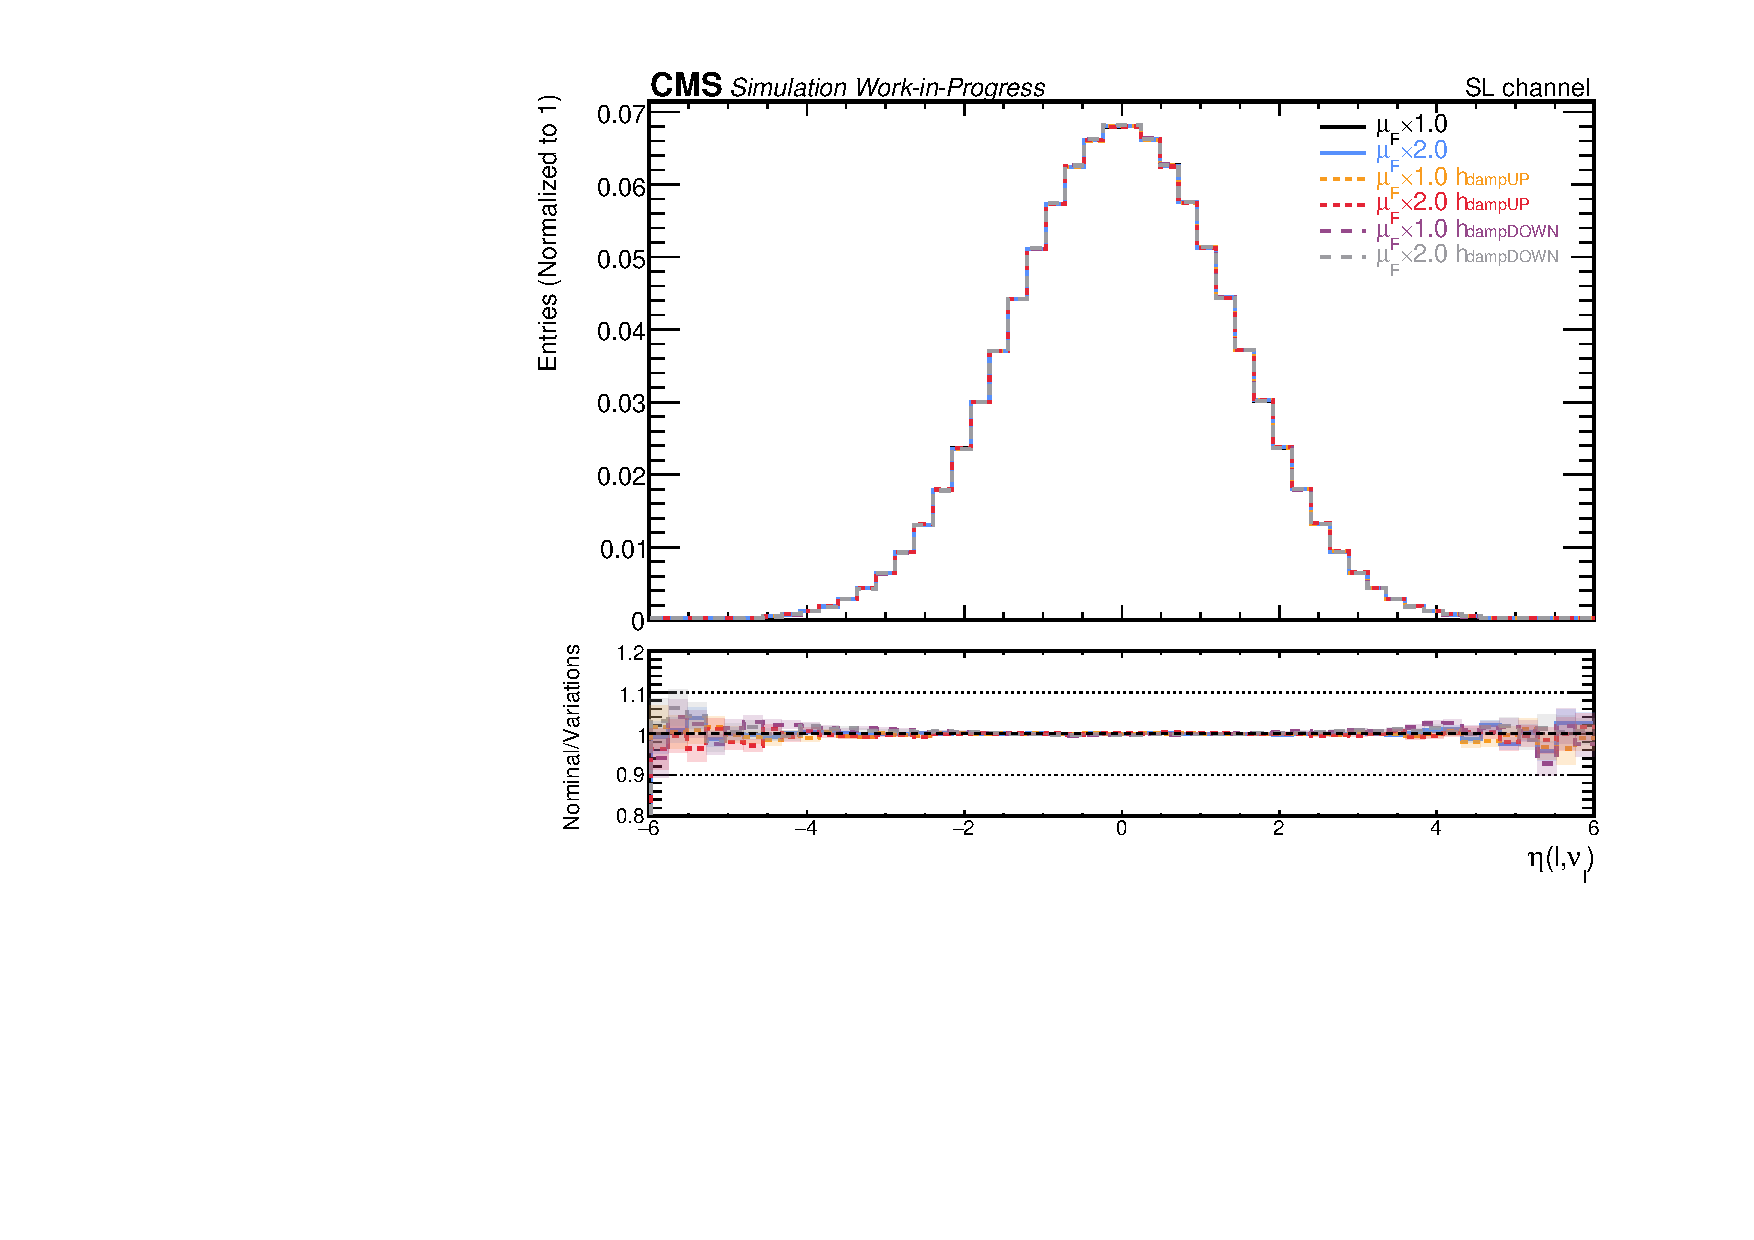
\includegraphics[width= 1.1\linewidth]{DL/ratio_leptons_pseudorapidity.pdf}
        \caption{}
        \label{app:subfig:eta(leptons)_DL}
    \end{subfigure}
    \caption{Distributions of (a) energy, (b) transverse momentum,  (c) azimuthal angle and (d) pseudorapidity of all the leptons (charged and neutral) for the six different settings used in the simulation. The lower panel shows the ratio of the nominal setting to the variations. The shaded bands represent statistical uncertainties. The last bins contain the overflow events.}
    \label{app:fig:leptons_DL}
\end{figure}


\begin{figure}[H]
    \centering
    \begin{subfigure}{0.49\textwidth}
        \centering
        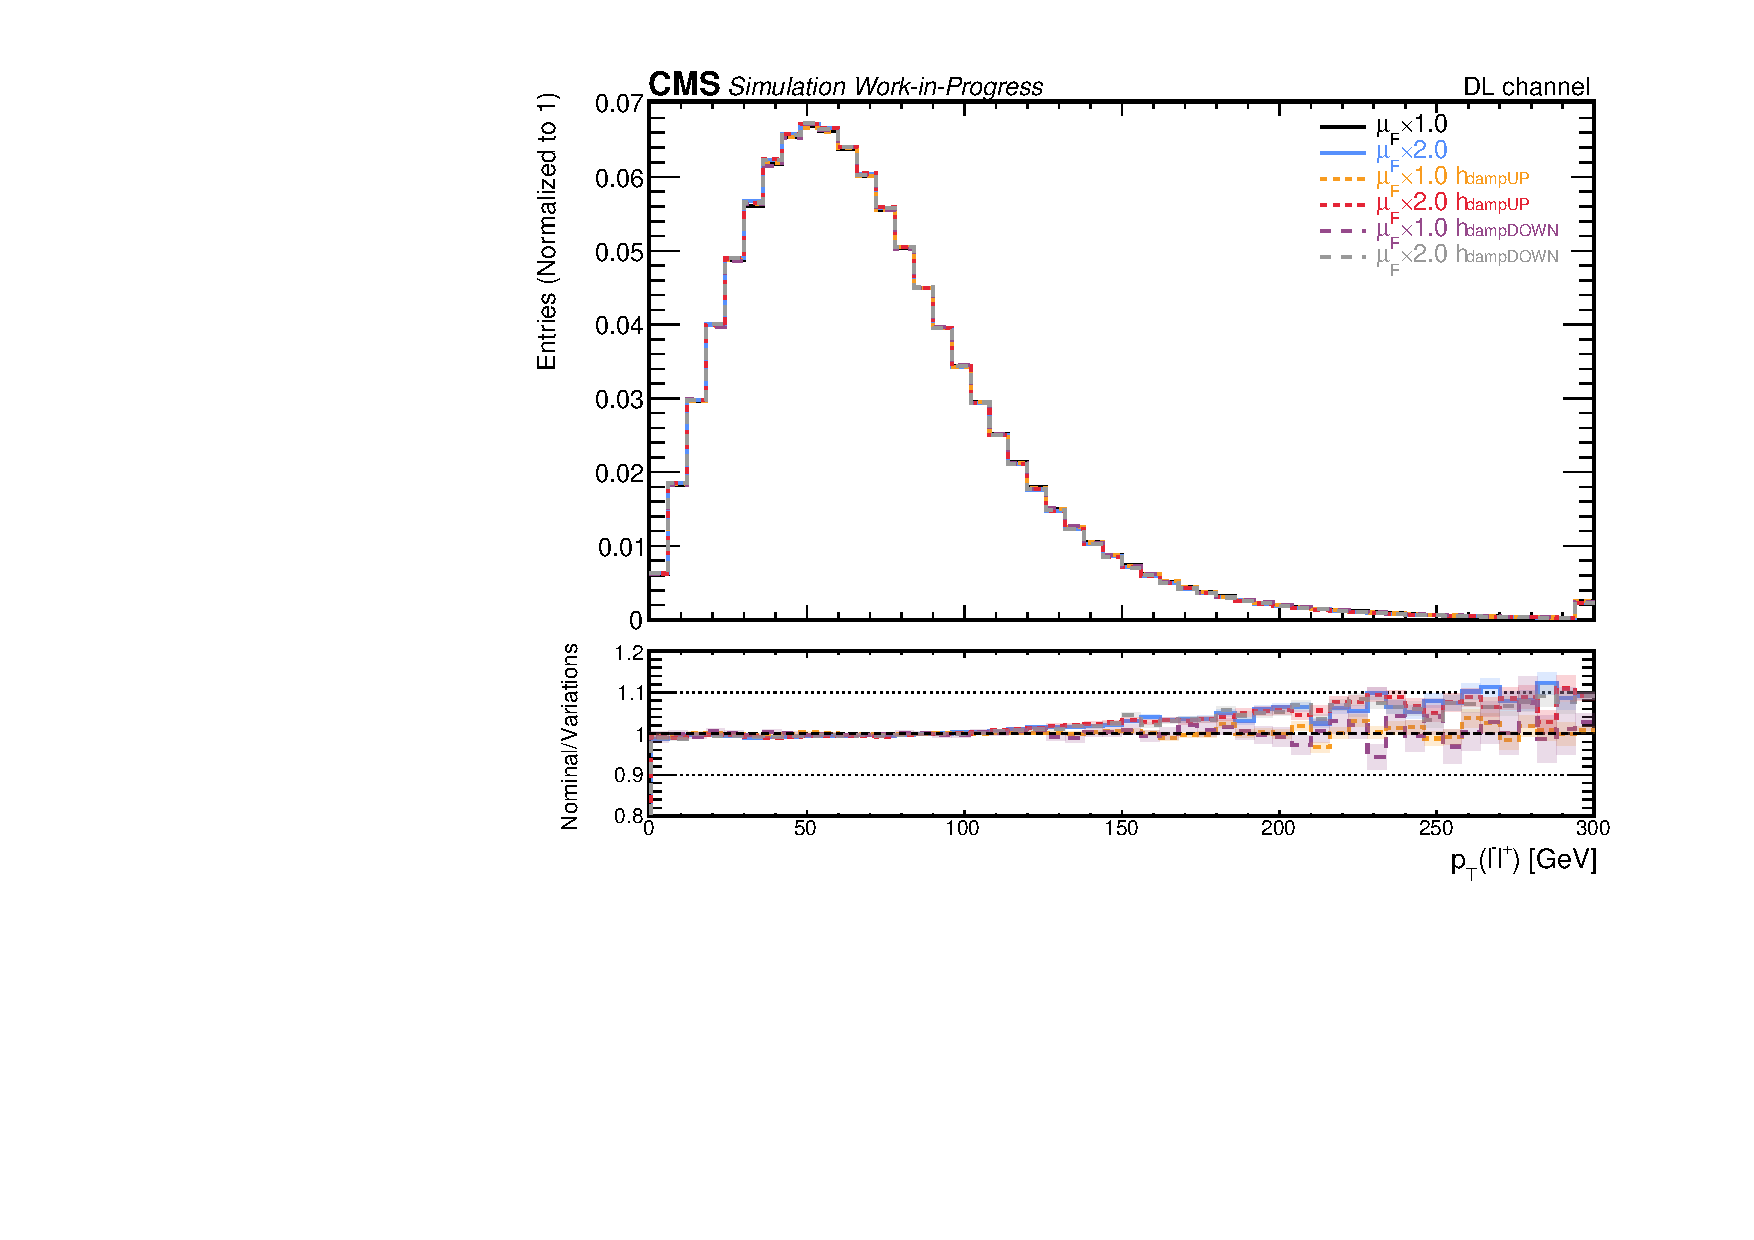
\includegraphics[width= 1.1\linewidth]{DL/ratio_ll_system_pt.pdf}
        \caption{}
        \label{app:subfig:pt(ll)_DL}
    \end{subfigure}
    \begin{subfigure}{0.49\textwidth}
        \centering
        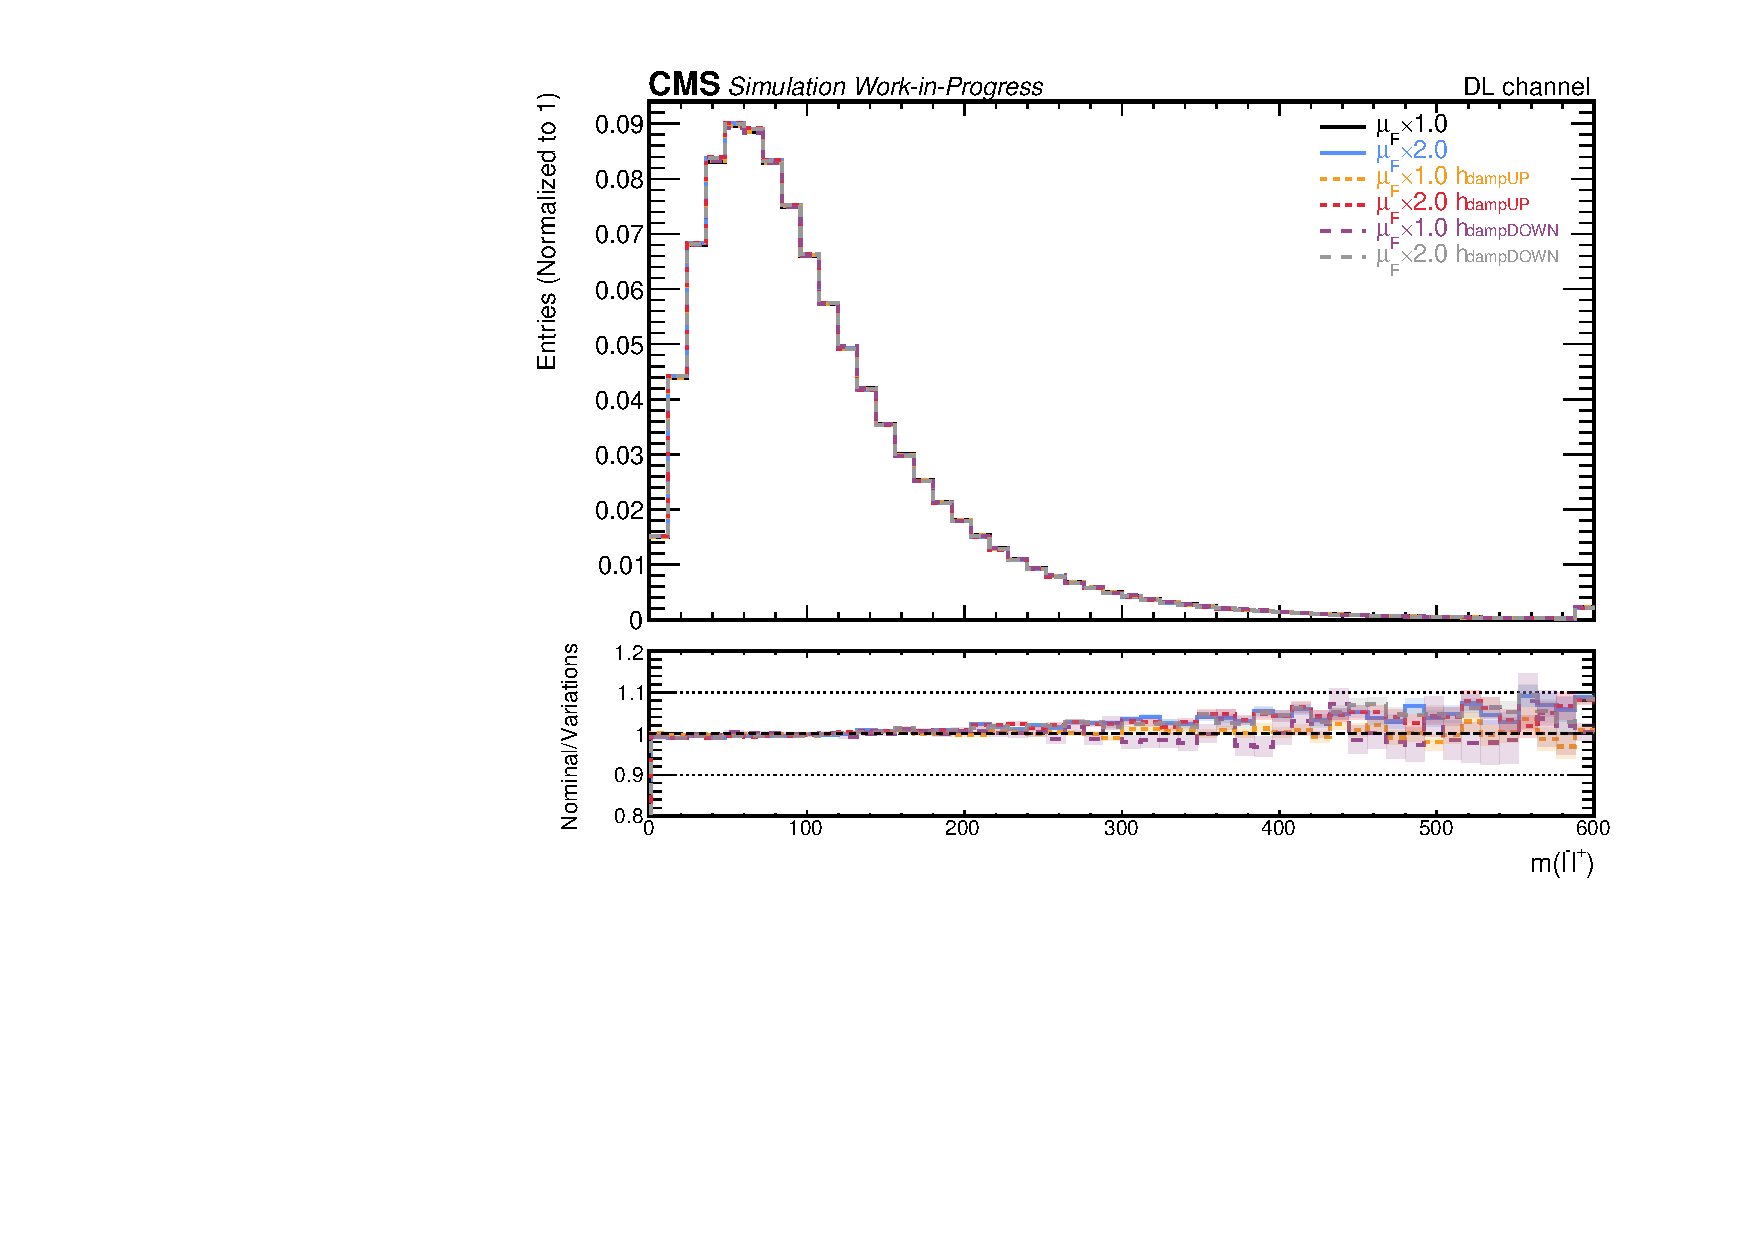
\includegraphics[width= 1.1\linewidth]{DL/ratio_ll_system_invariant_mass.pdf}
        \caption{}
        \label{app:subfig:m(ll)_DL}
    \end{subfigure}

    \vspace{0.2cm}
    
    \begin{subfigure}{0.49\textwidth}
        \centering
        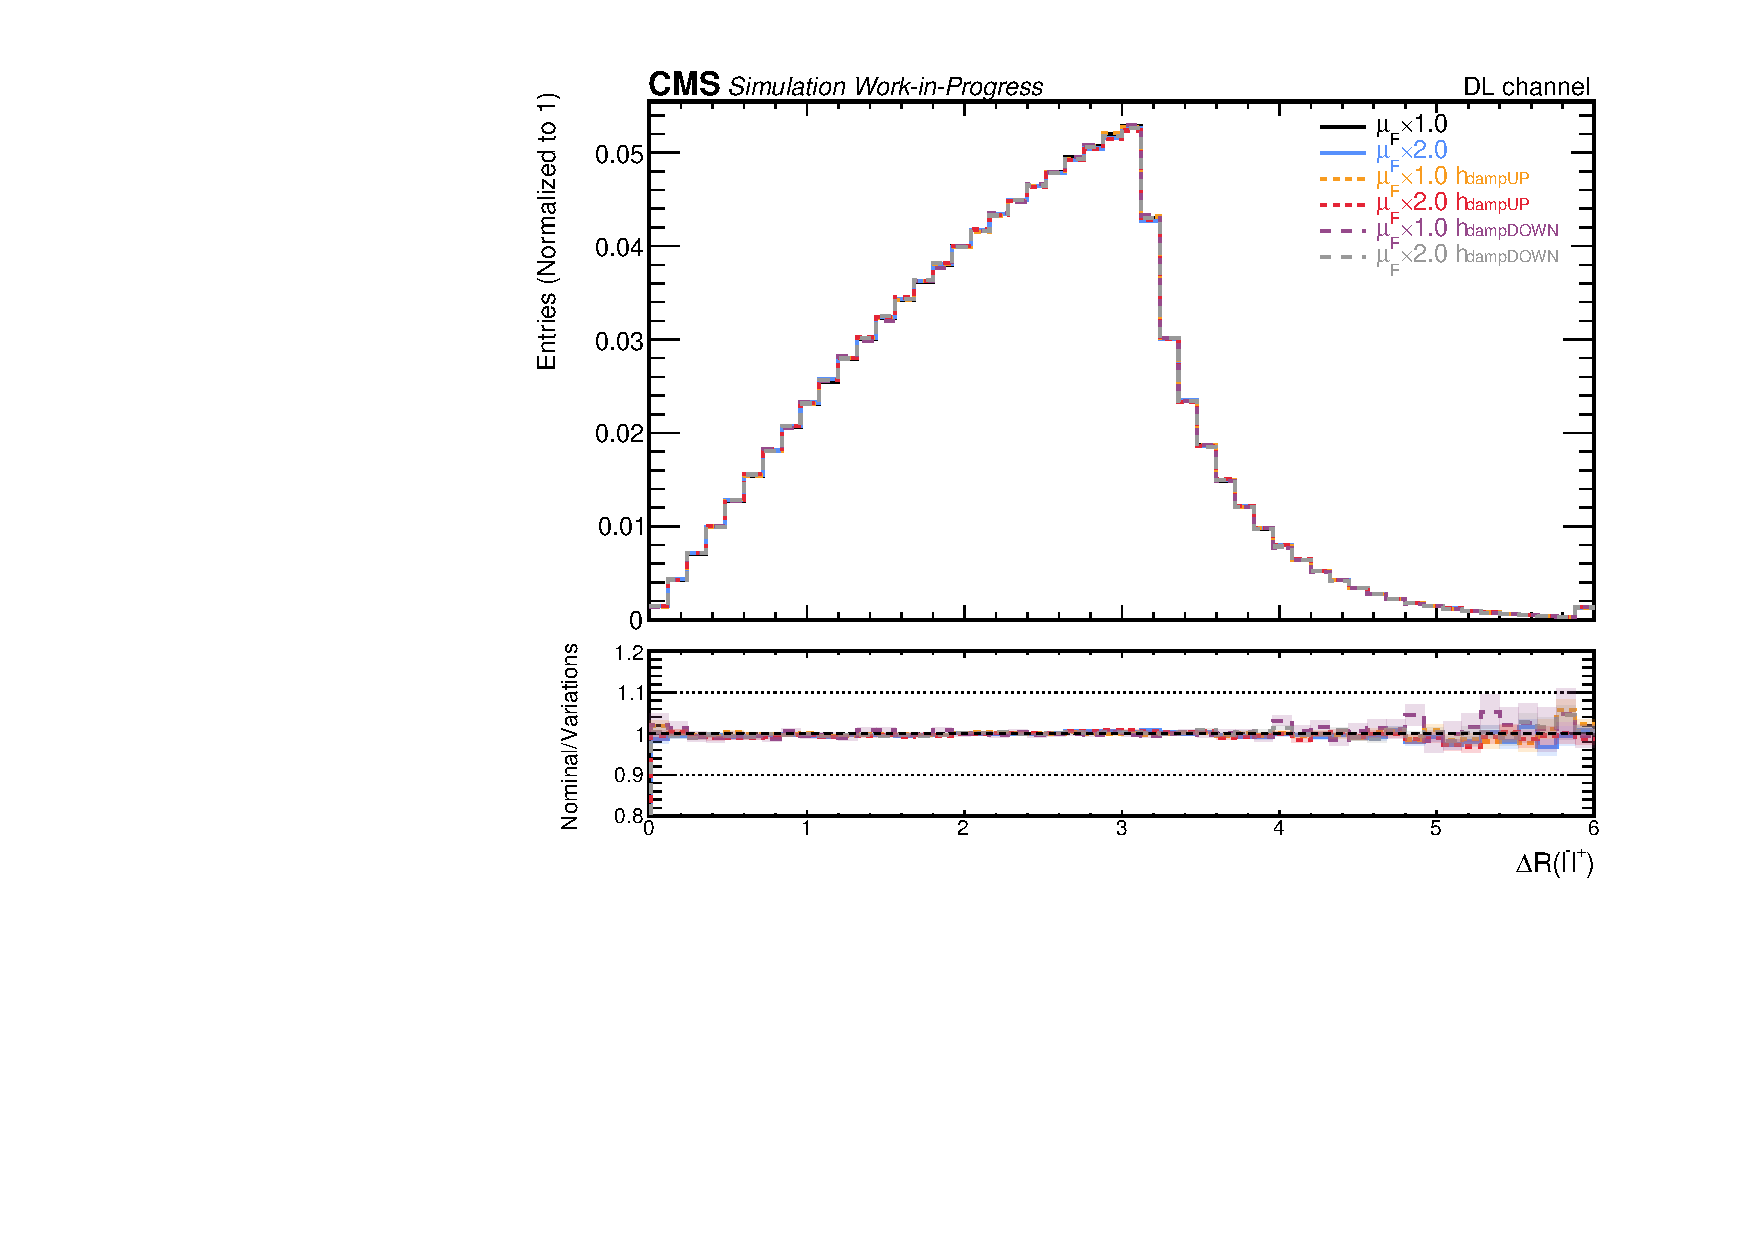
\includegraphics[width= 1.1\linewidth]{DL/ratio_ll_system_dR.pdf}
        \caption{}
        \label{app:subfig:dR(ll)_DL}
    \end{subfigure}
    \begin{subfigure}{0.49\textwidth}
        \centering
        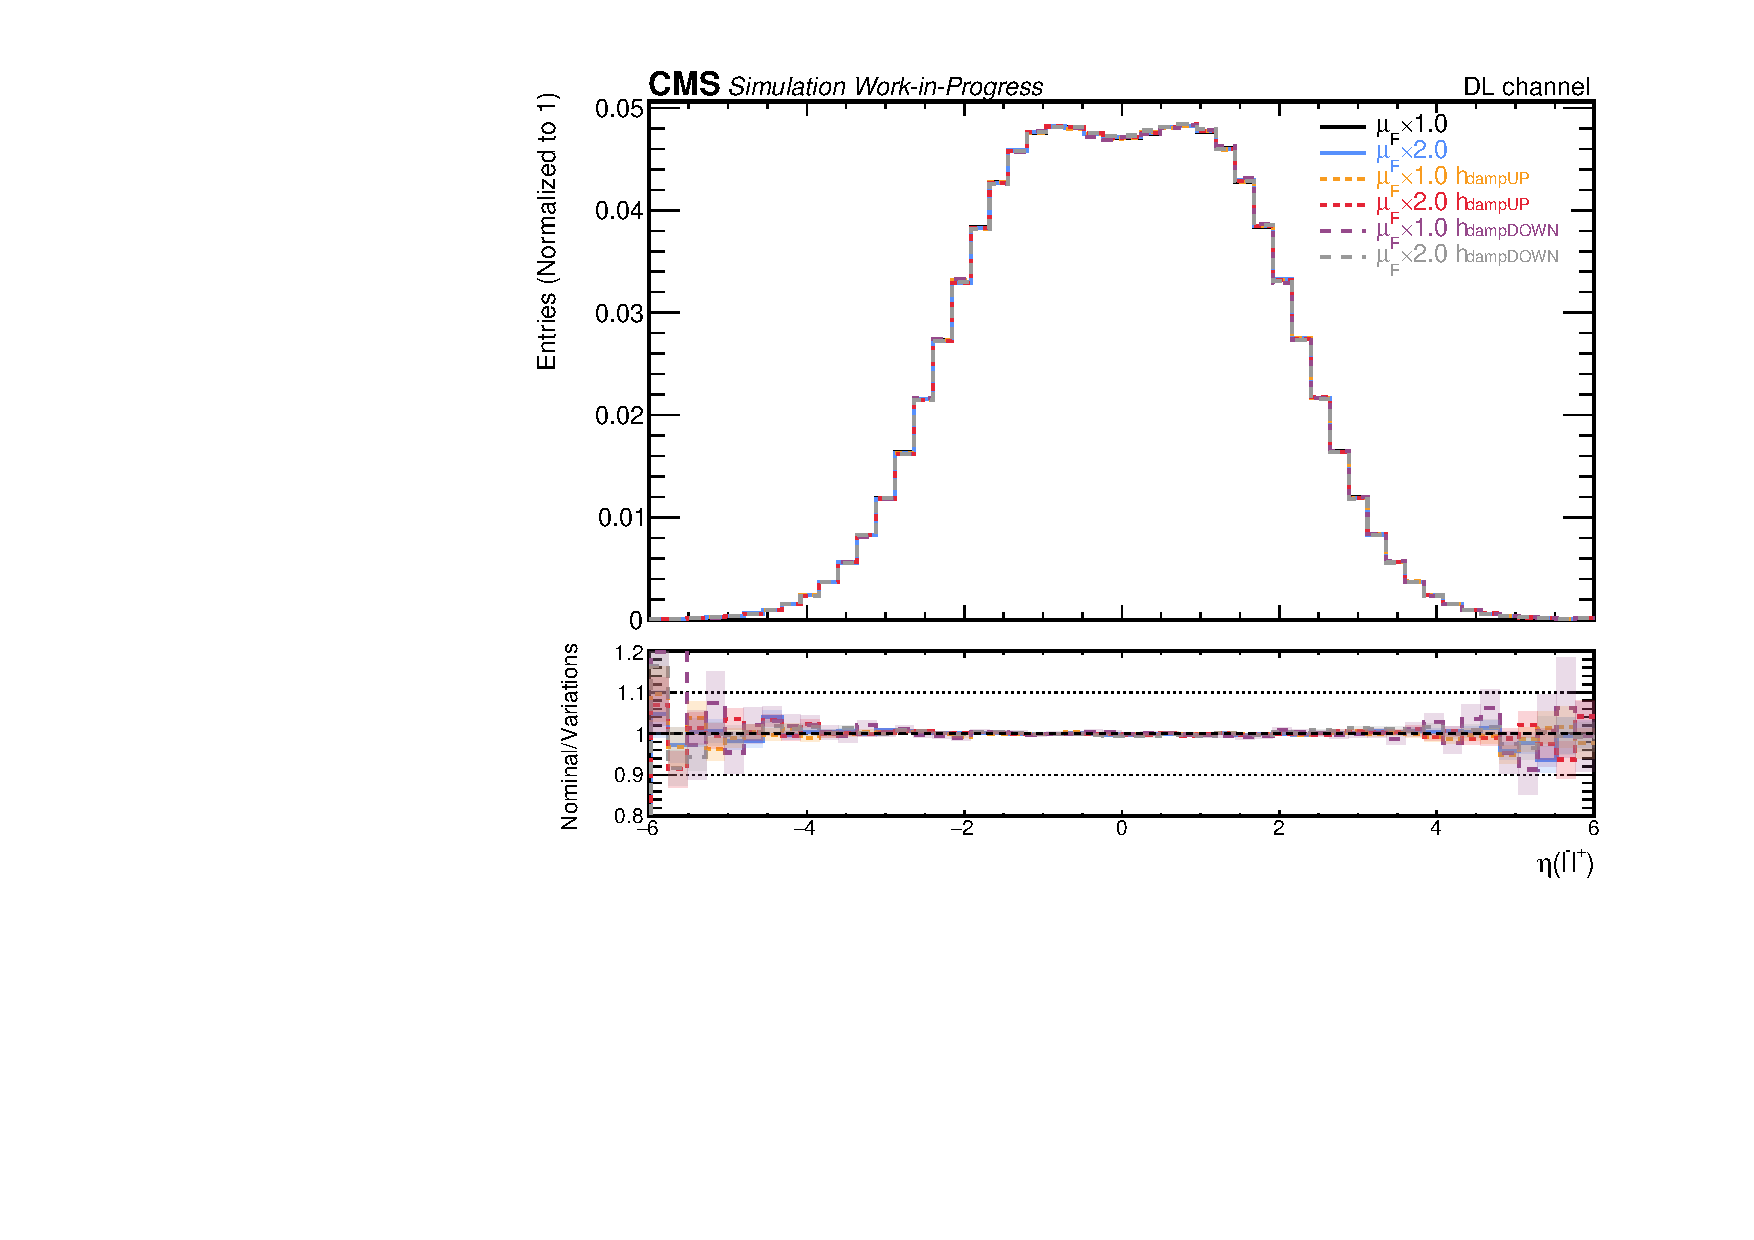
\includegraphics[width= 1.1\linewidth]{DL/ratio_ll_system_pseudorapidity.pdf}
        \caption{}
        \label{app:subfig:eta(ll)_DL}
    \end{subfigure}
    \caption{Distributions of (a) transverse momentum, (b) invariant mass,  (c) angular separation and (d) rapidity of the $\ell^-\ell^+$ system for the six different settings used in the simulation. The lower panel shows the ratio of the nominal setting to the variations. The shaded bands represent statistical uncertainties. The last bins contain the overflow events.}
    \label{app:fig:ll_DL}
\end{figure}



\begin{figure}[H]
    \centering
    \begin{subfigure}{0.49\textwidth}
        \centering
        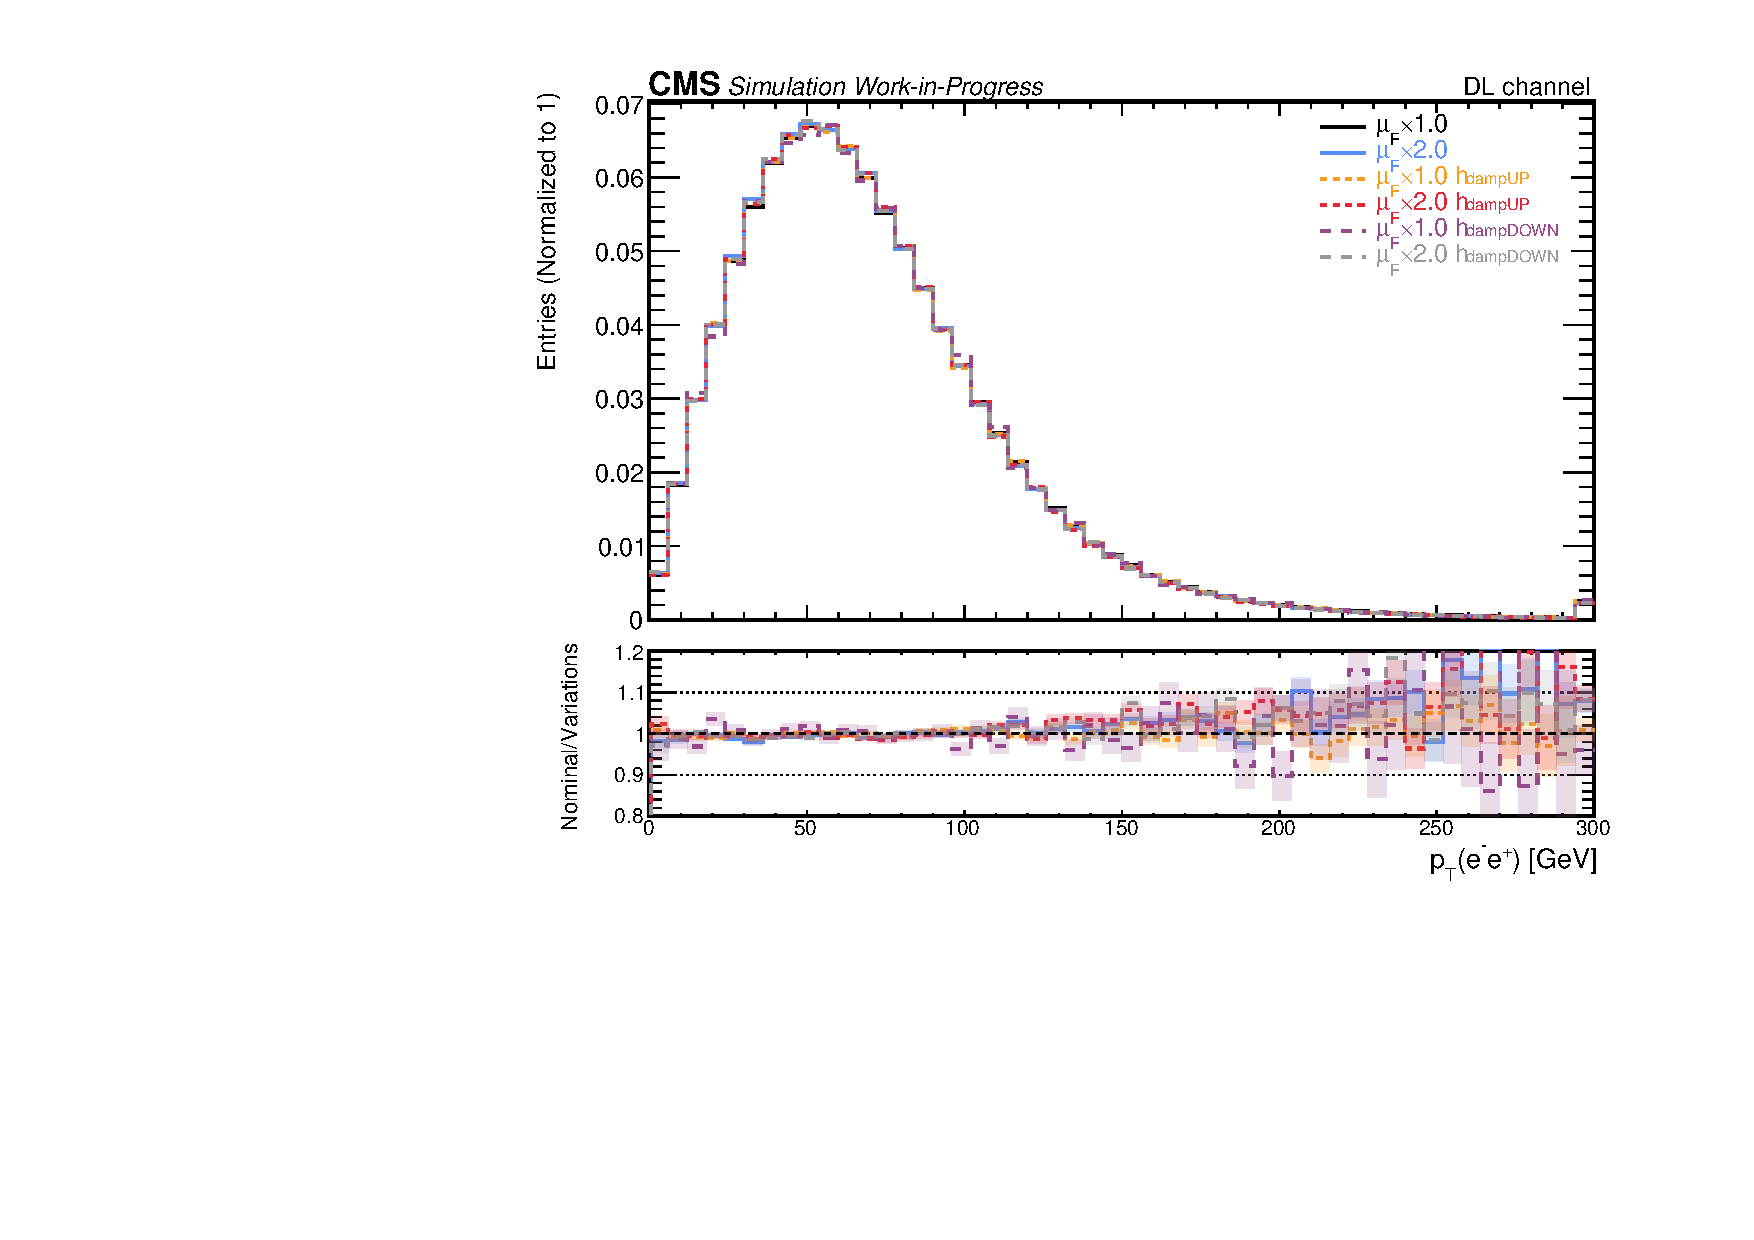
\includegraphics[width= 1.1\linewidth]{DL/ratio_ee_system_pt.pdf}
        \caption{}
        \label{app:subfig:pt(ee)_DL}
    \end{subfigure}
    \begin{subfigure}{0.49\textwidth}
        \centering
        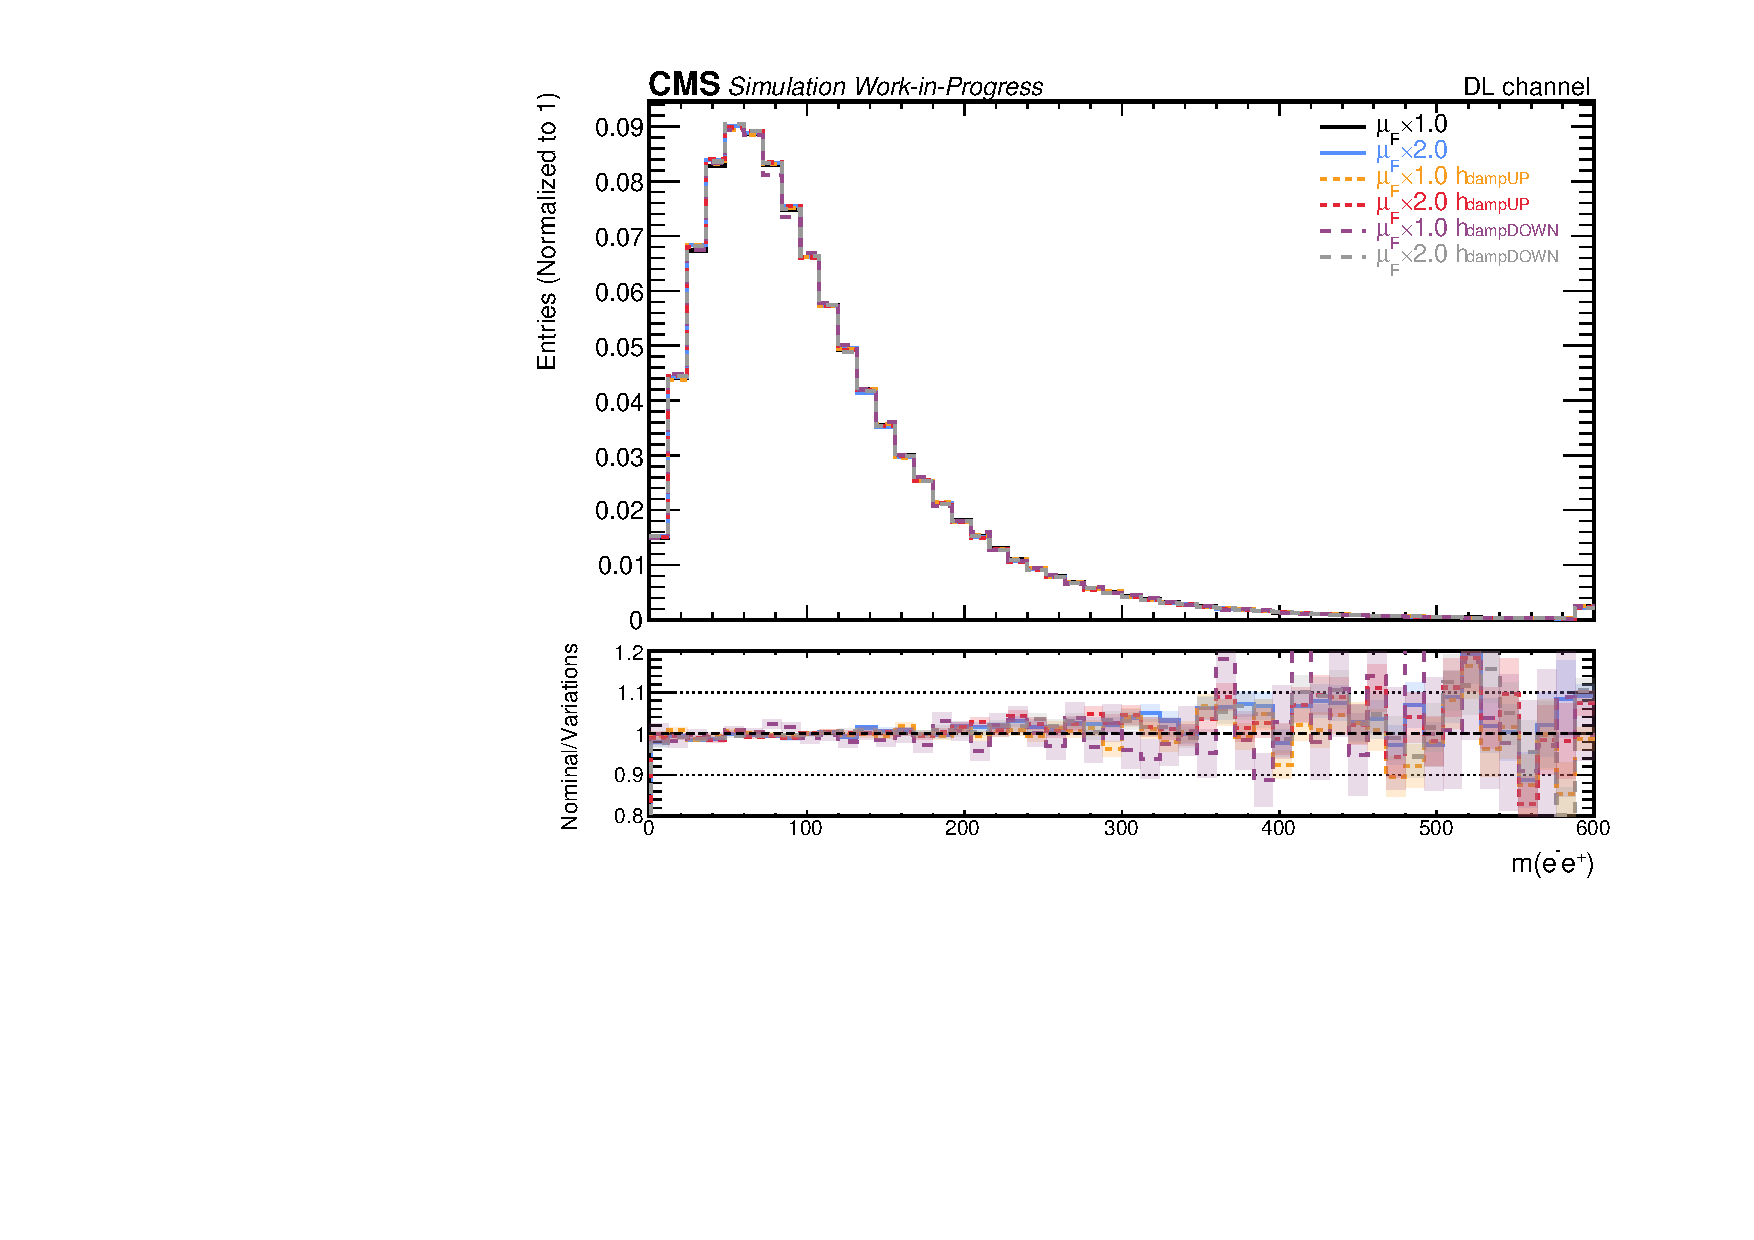
\includegraphics[width= 1.1\linewidth]{DL/ratio_ee_system_invariant_mass.pdf}
        \caption{}
        \label{app:subfig:m(ee)_DL}
    \end{subfigure}

    \vspace{0.2cm}
    
    \begin{subfigure}{0.49\textwidth}
        \centering
        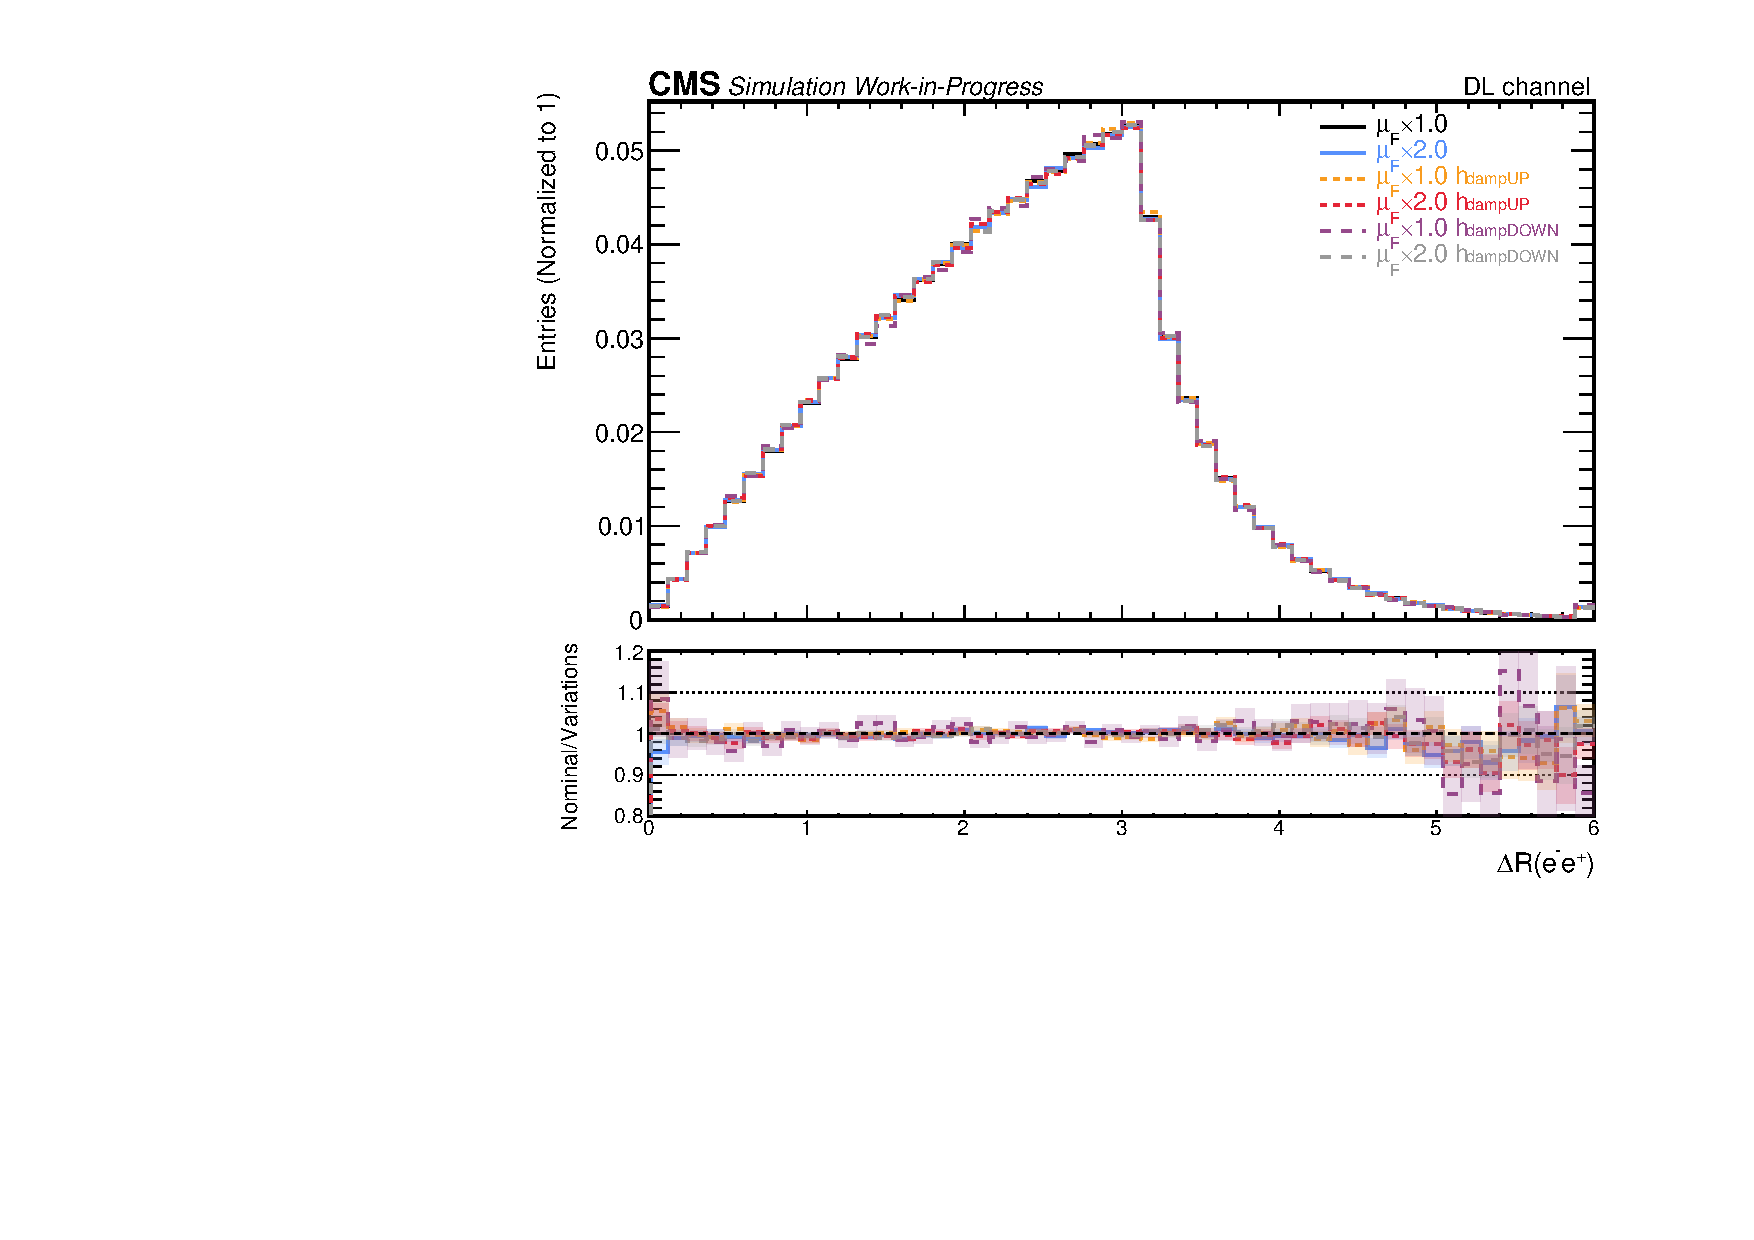
\includegraphics[width= 1.1\linewidth]{DL/ratio_ee_system_dR.pdf}
        \caption{}
        \label{app:subfig:dR(ee)_DL}
    \end{subfigure}
    \begin{subfigure}{0.49\textwidth}
        \centering
        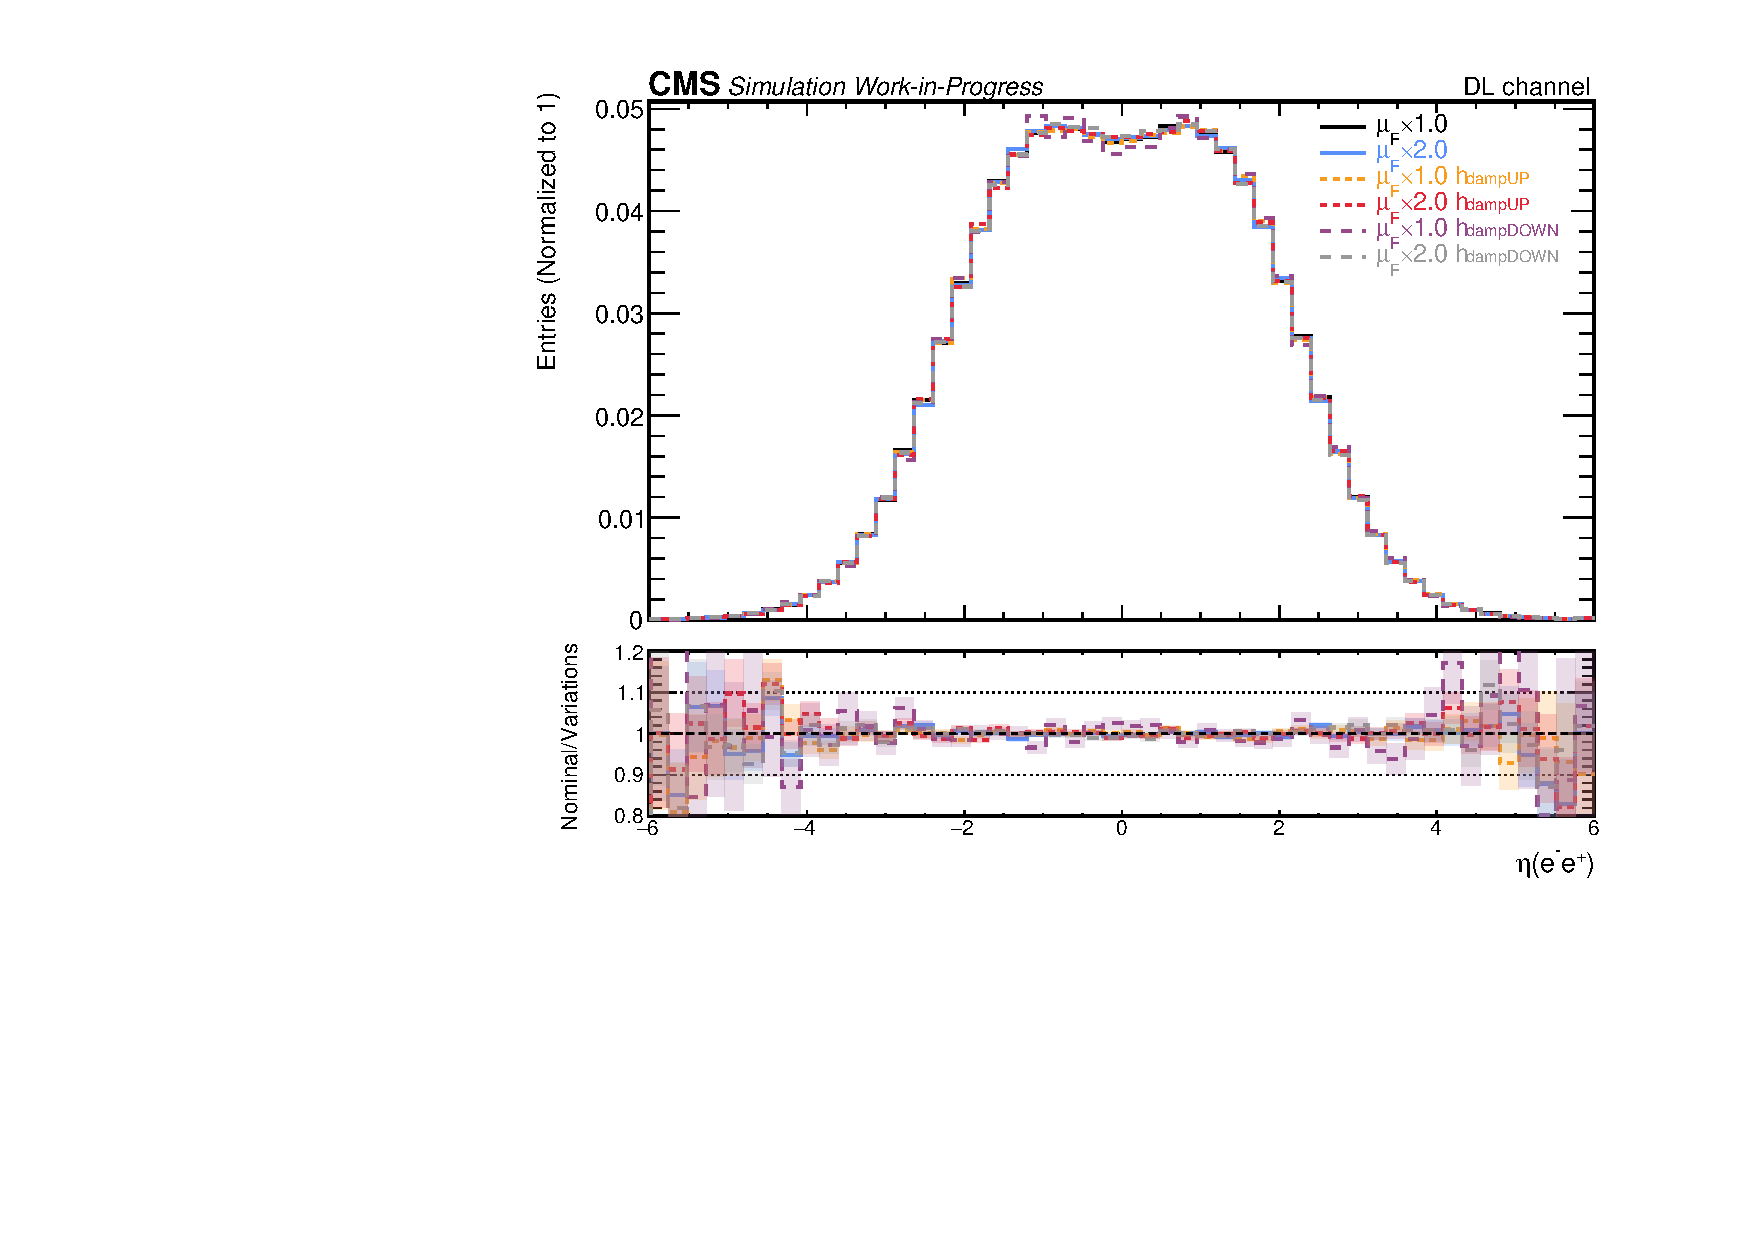
\includegraphics[width= 1.1\linewidth]{DL/ratio_ee_system_pseudorapidity.pdf}
        \caption{}
        \label{app:subfig:eta(ee)_DL}
    \end{subfigure}
    \caption{Distributions of (a) transverse momentum, (b) invariant mass,  (c) angular separation and (d) rapidity of the $e^-e^+$ system for the six different settings used in the simulation. The lower panel shows the ratio of the nominal setting to the variations. The shaded bands represent statistical uncertainties. The last bins contain the overflow events.}
    \label{app:fig:ee_DL}
\end{figure}


\begin{figure}[H]
    \centering
    \begin{subfigure}{0.49\textwidth}
        \centering
        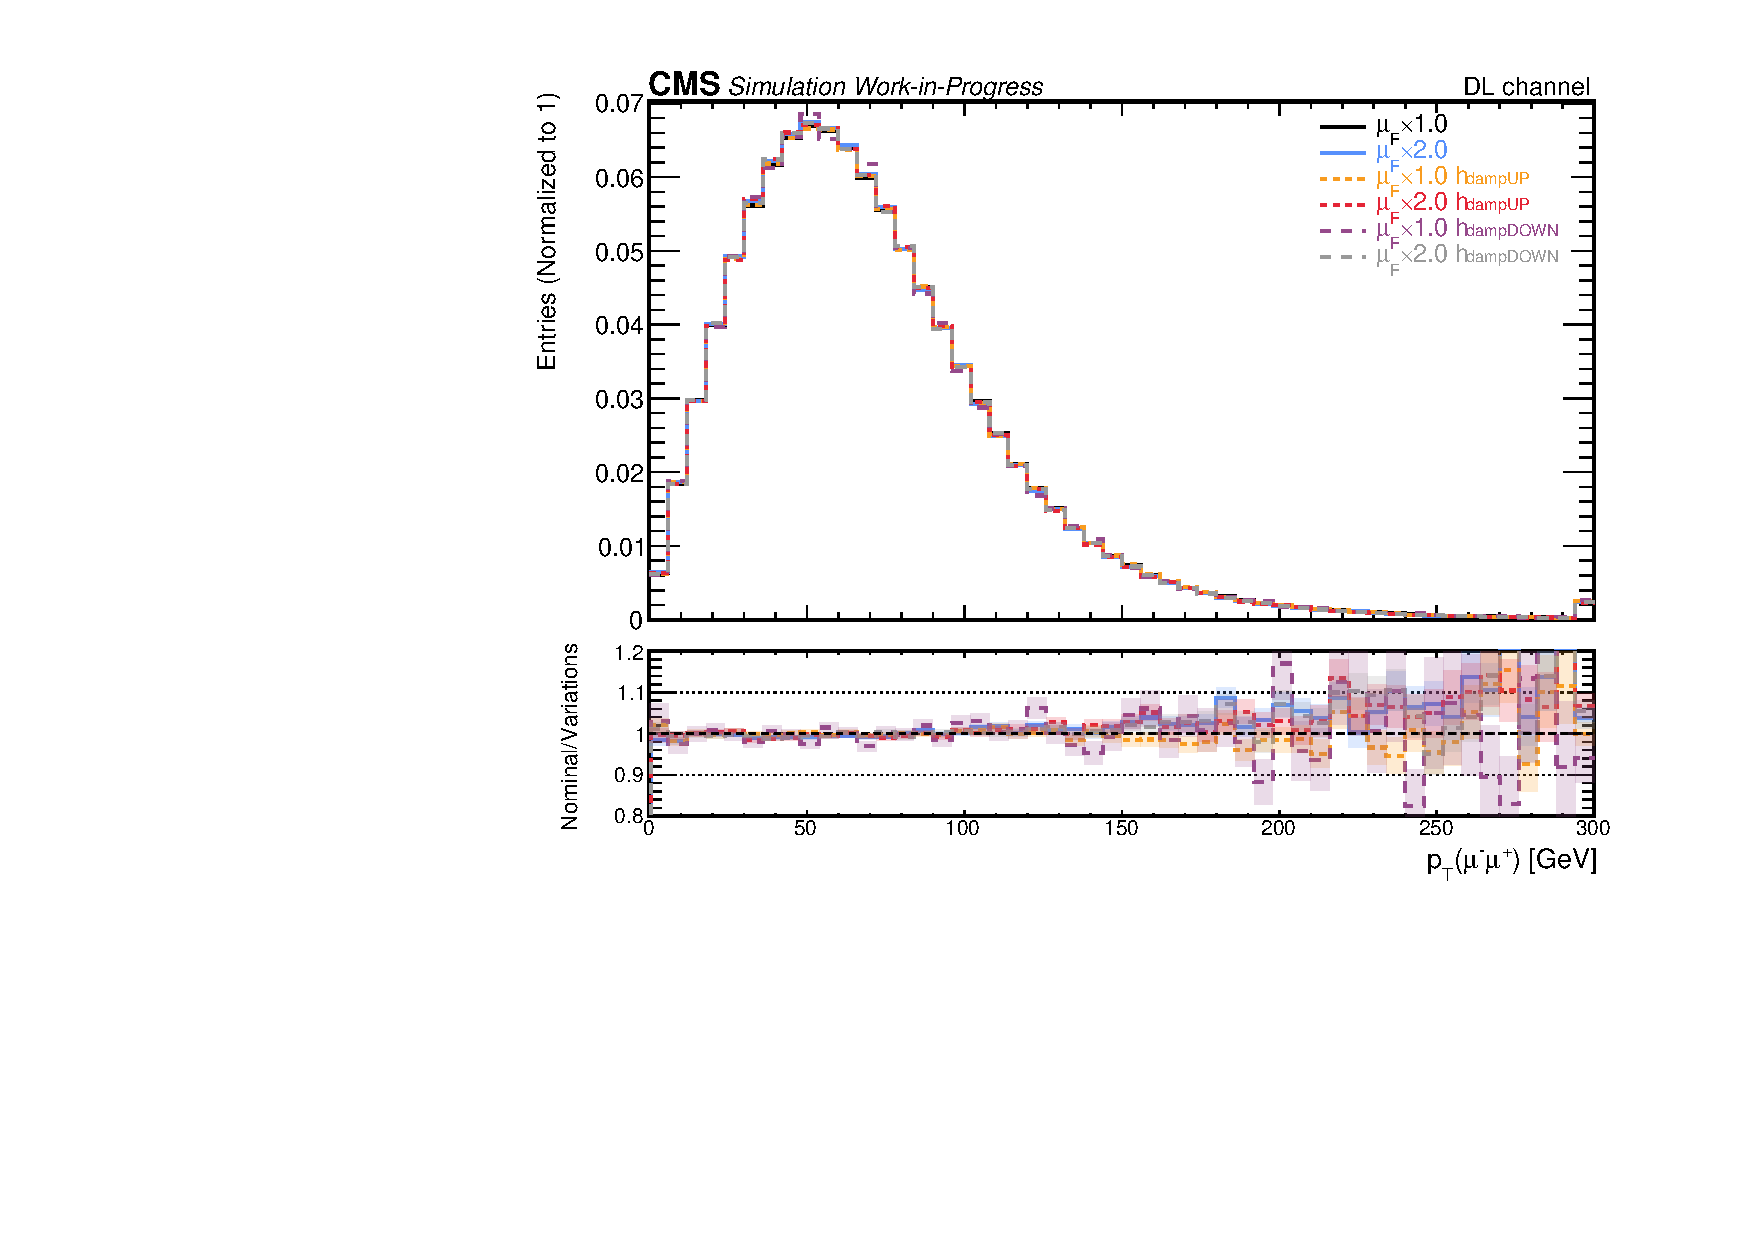
\includegraphics[width= 1.1\linewidth]{DL/ratio_mm_system_pt.pdf}
        \caption{}
        \label{app:subfig:pt(mm)_DL}
    \end{subfigure}
    \begin{subfigure}{0.49\textwidth}
        \centering
        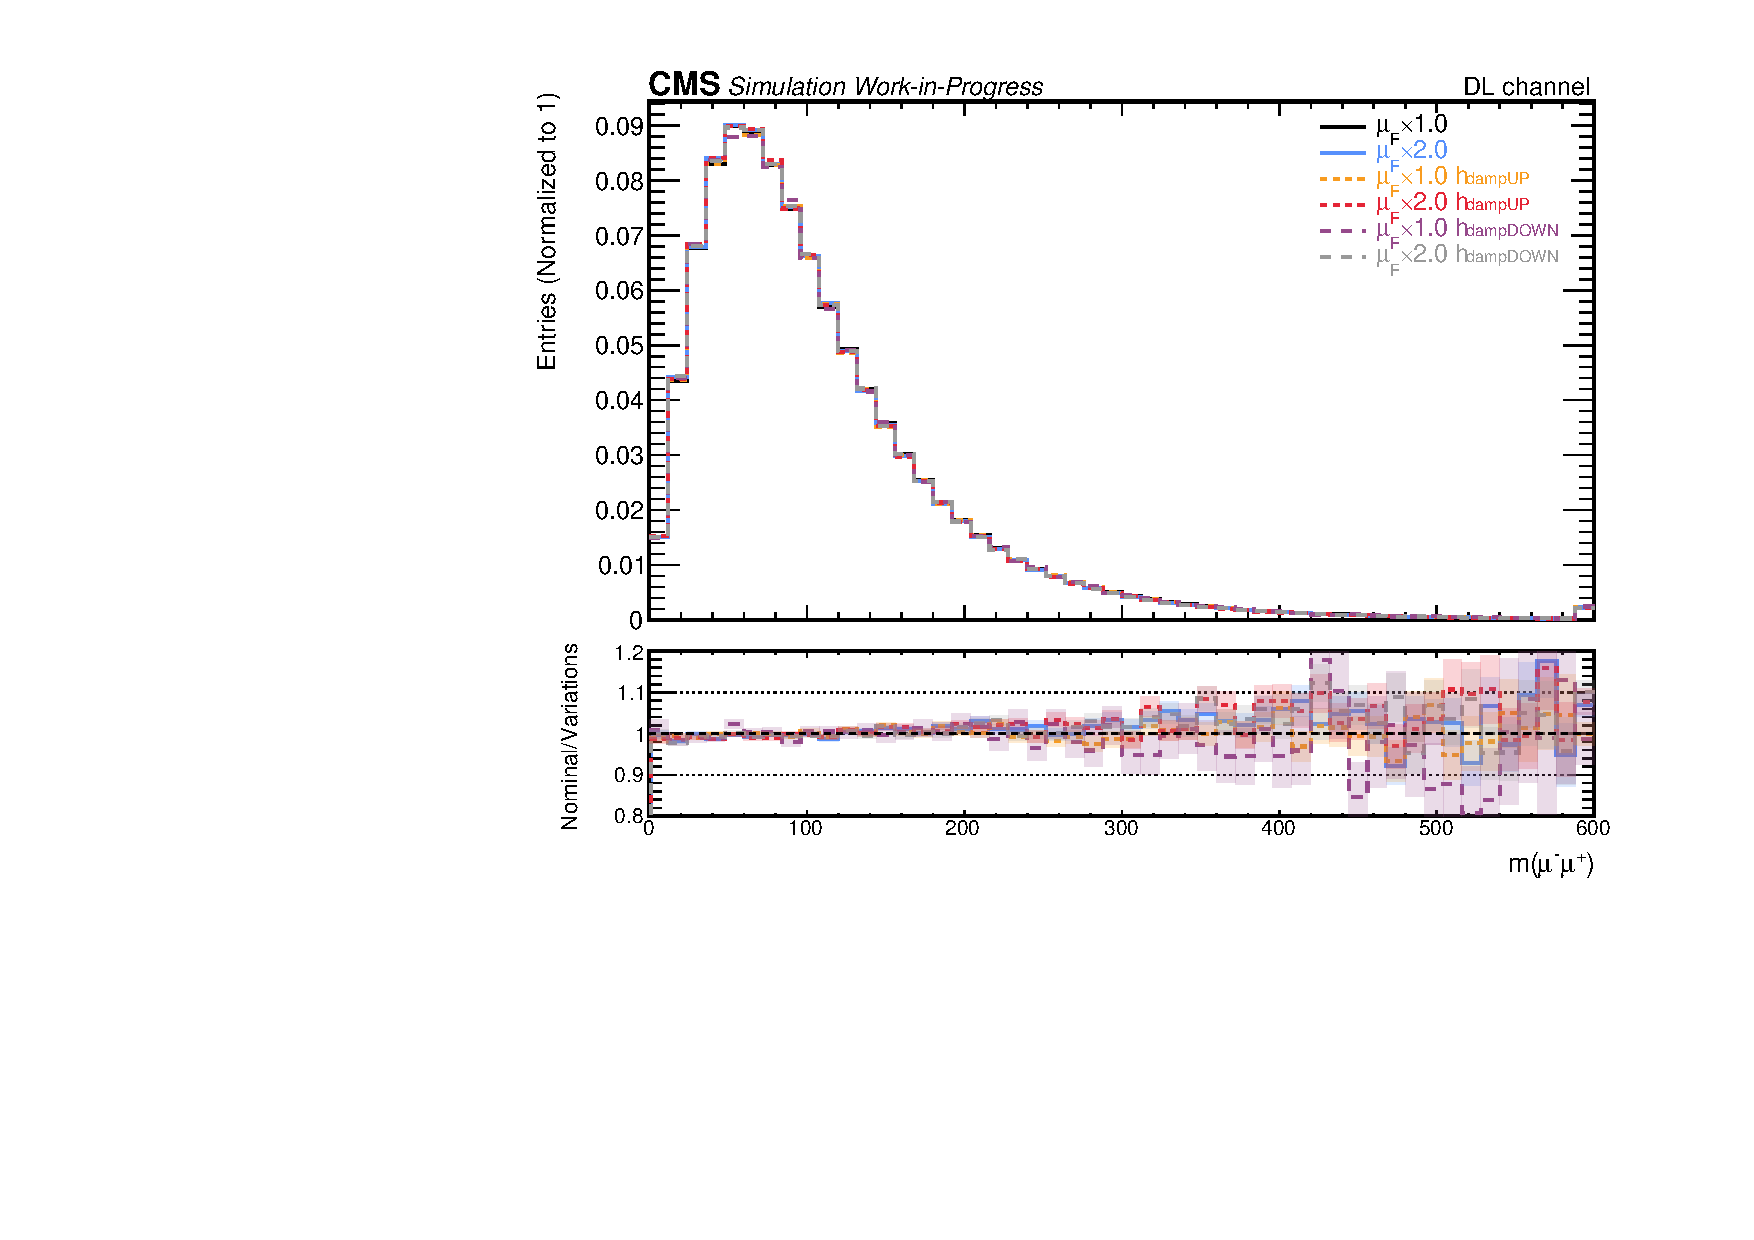
\includegraphics[width= 1.1\linewidth]{DL/ratio_mm_system_invariant_mass.pdf}
        \caption{}
        \label{app:subfig:m(mm)_DL}
    \end{subfigure}

    \vspace{0.2cm}
    
    \begin{subfigure}{0.49\textwidth}
        \centering
        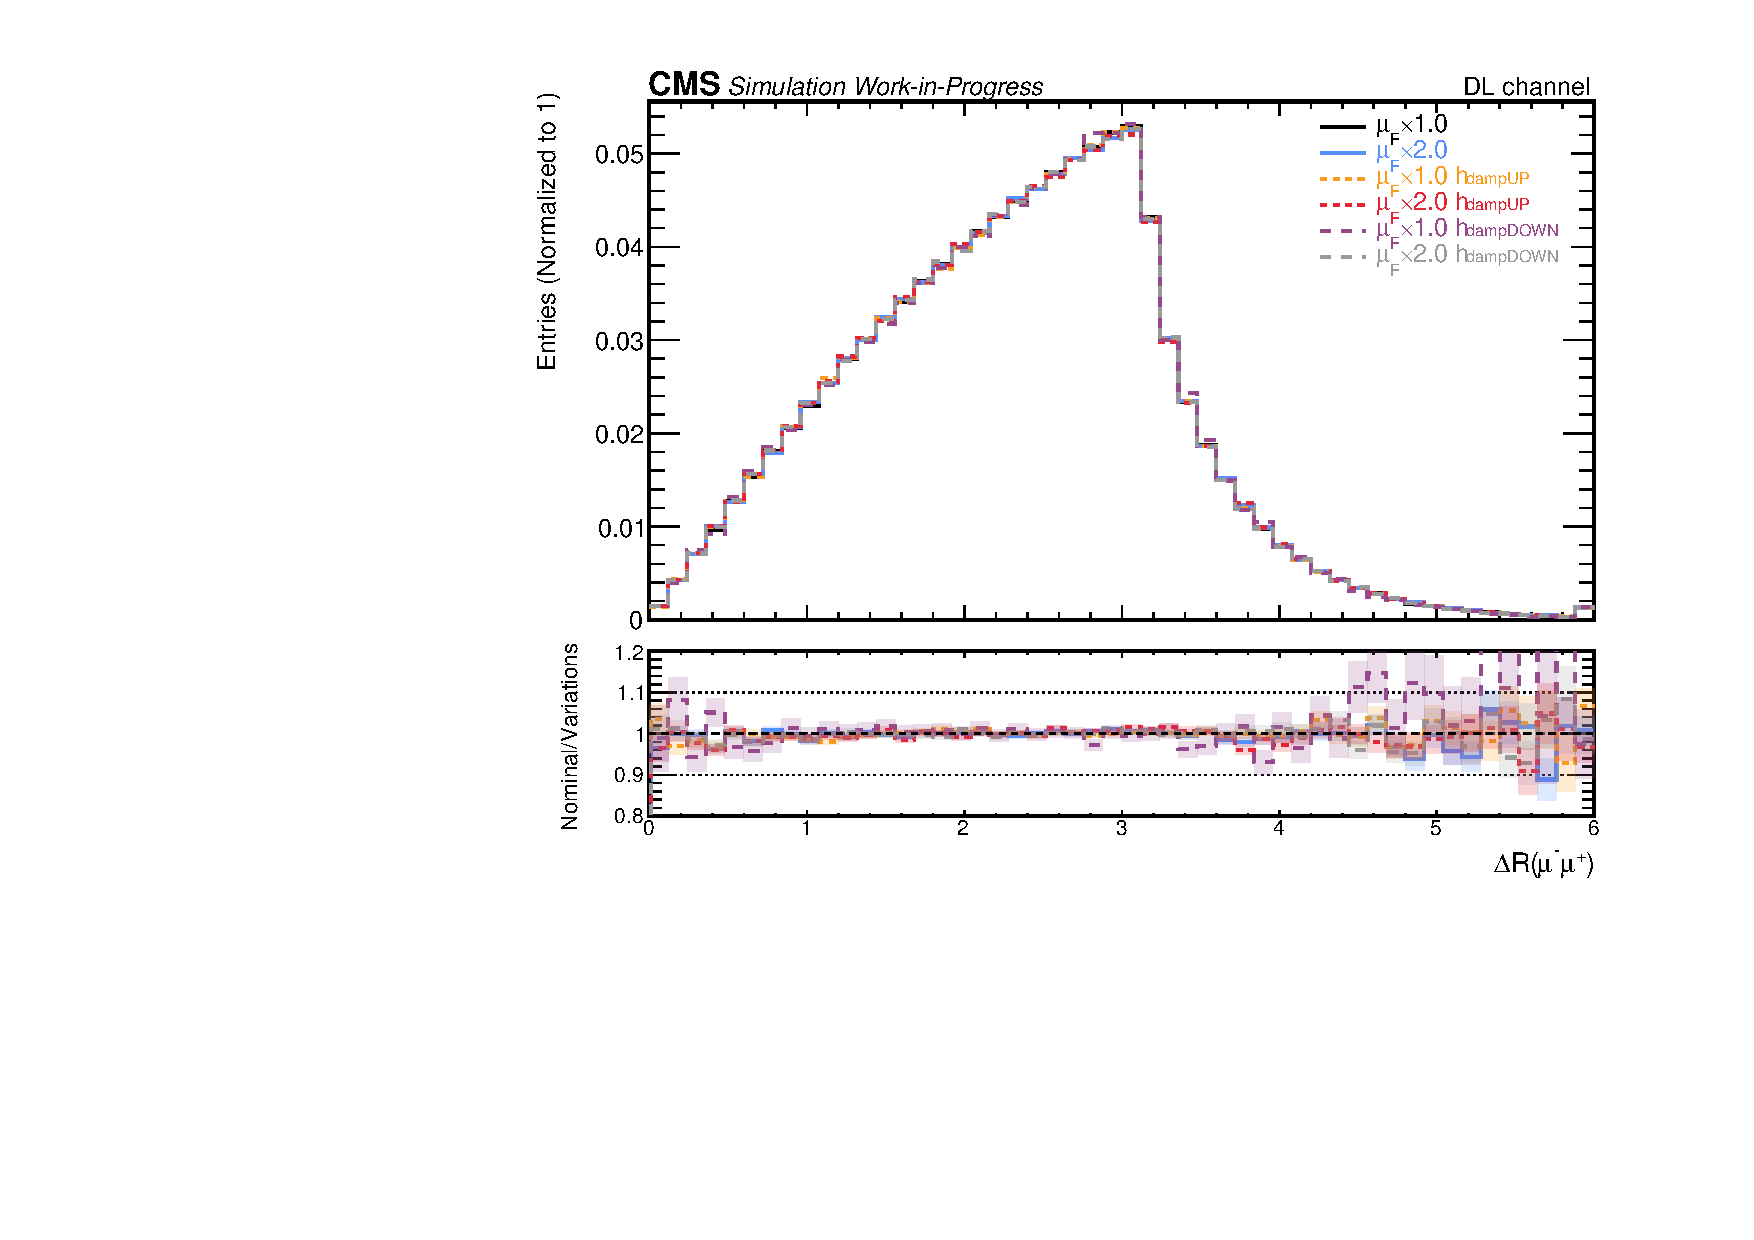
\includegraphics[width= 1.1\linewidth]{DL/ratio_mm_system_dR.pdf}
        \caption{}
        \label{app:subfig:dR(mm)_DL}
    \end{subfigure}
    \begin{subfigure}{0.49\textwidth}
        \centering
        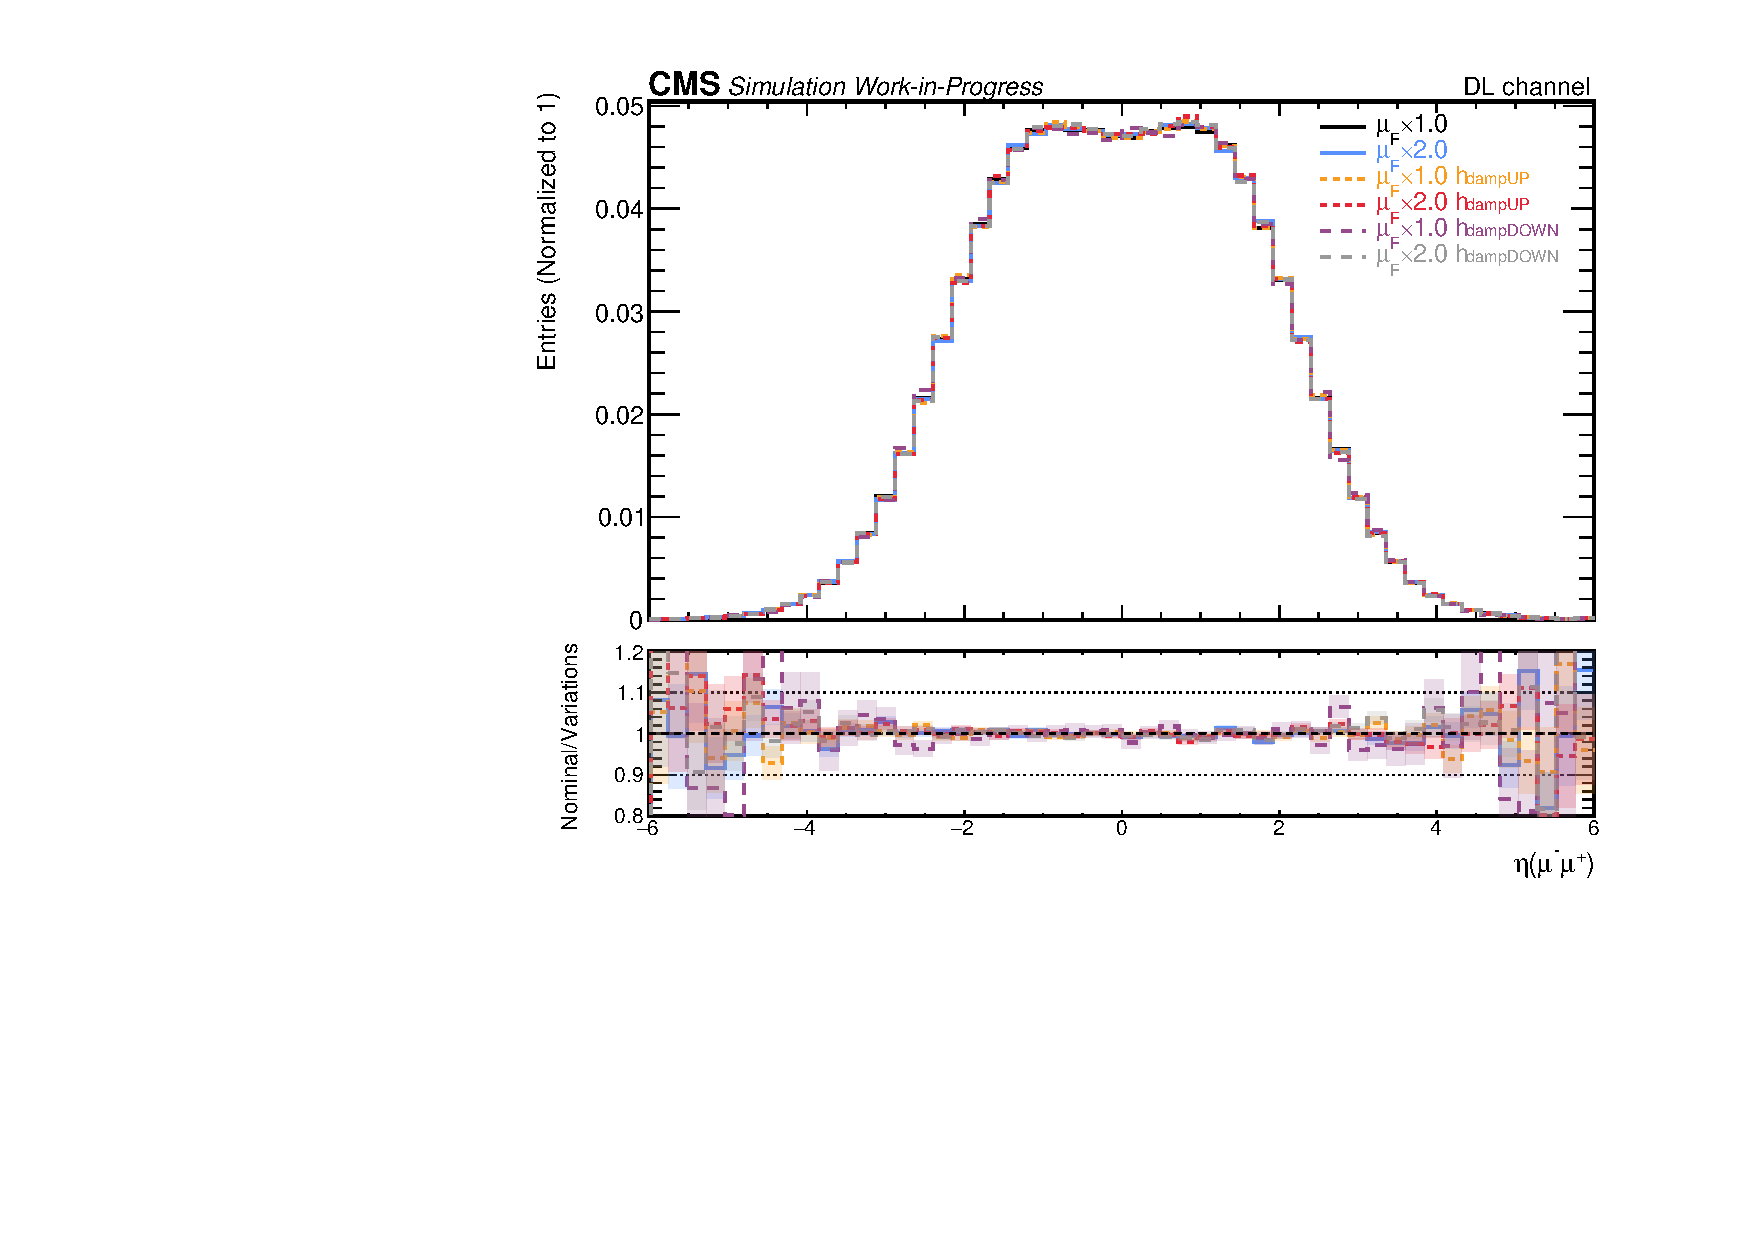
\includegraphics[width= 1.1\linewidth]{DL/ratio_mm_system_pseudorapidity.pdf}
        \caption{}
        \label{app:subfig:eta(mm)_DL}
    \end{subfigure}
    \caption{Distributions of (a) transverse momentum, (b) invariant mass,  (c) angular separation and (d) rapidity of the $\mu^-\mu^+$ system for the six different settings used in the simulation. The lower panel shows the ratio of the nominal setting to the variations. The shaded bands represent statistical uncertainties. The last bins contain the overflow events.}
    \label{app:fig:mumu_DL}
\end{figure}

\begin{figure}[H]
    \centering
    \begin{subfigure}{0.49\textwidth}
        \centering
        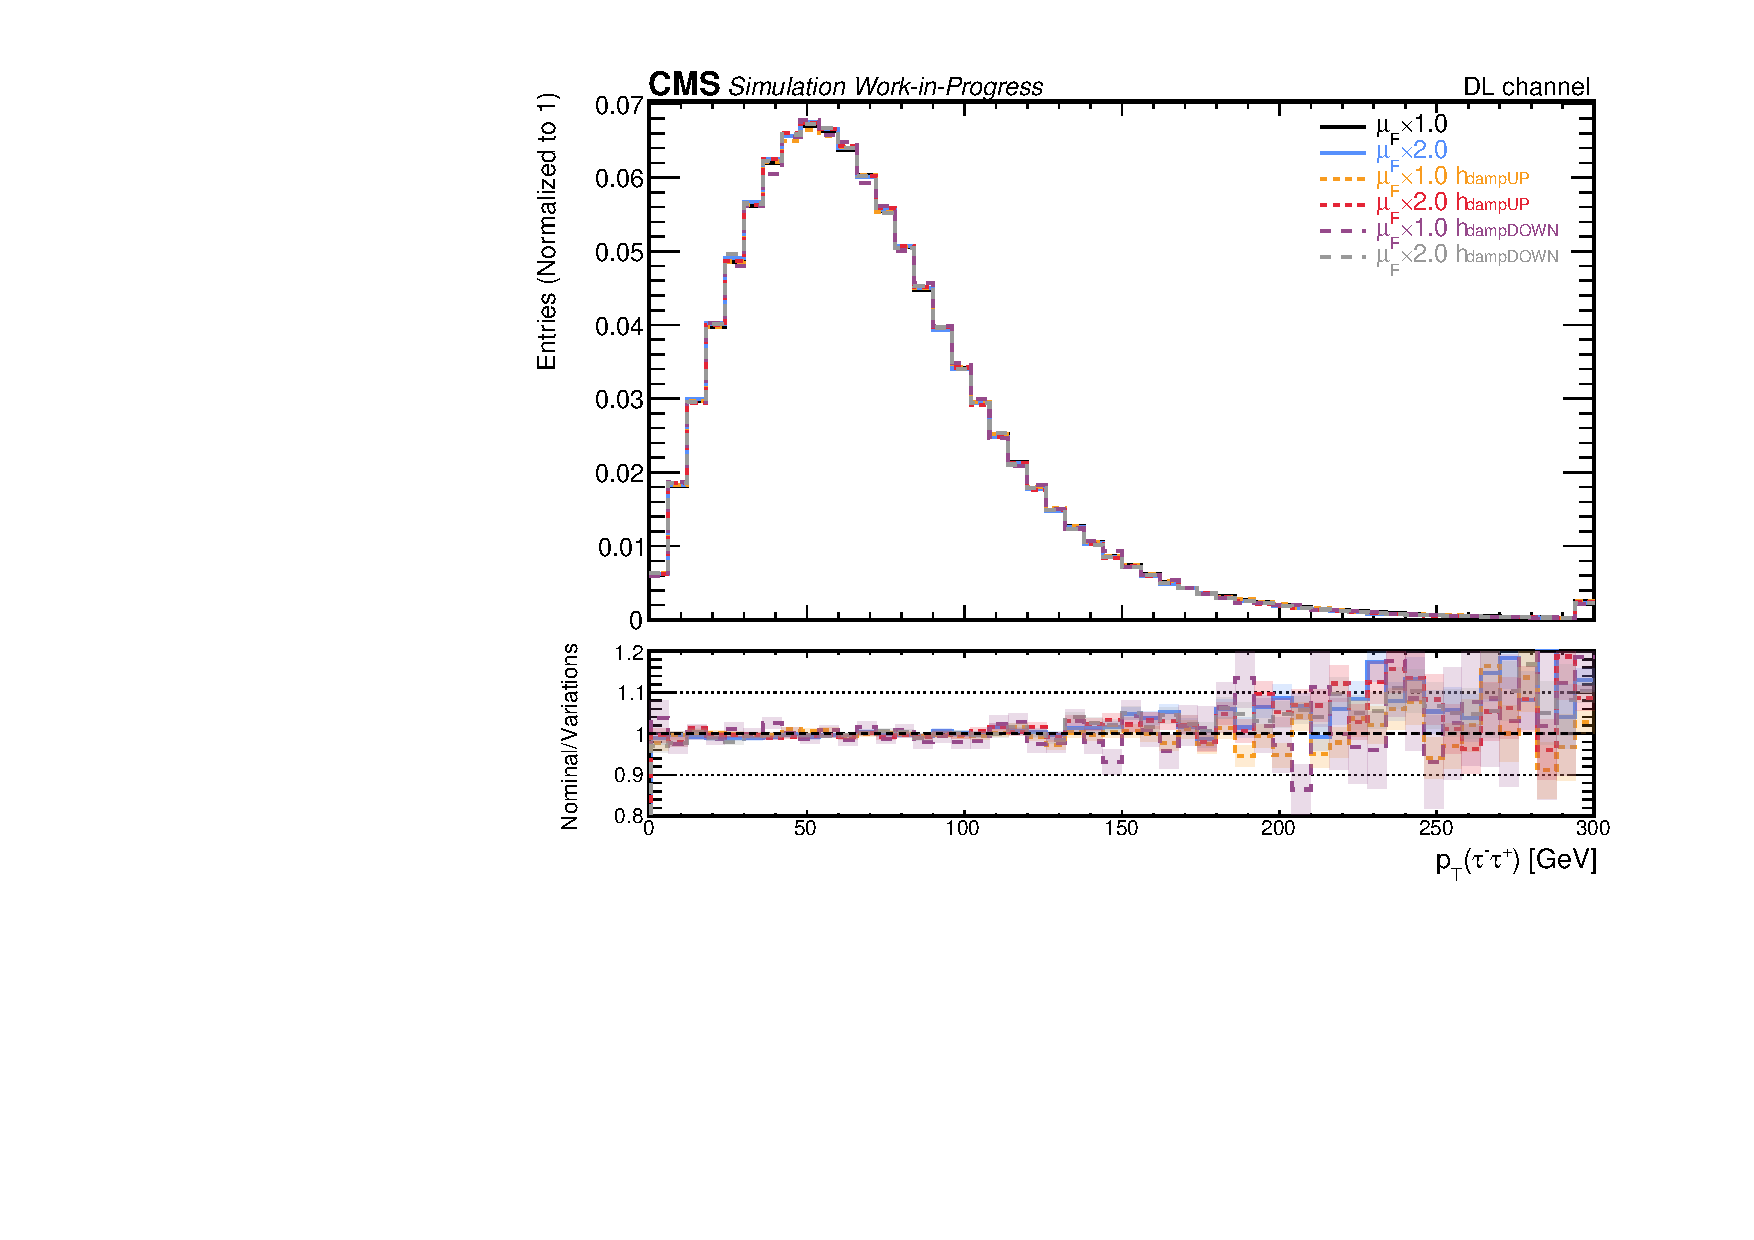
\includegraphics[width= 1.1\linewidth]{DL/ratio_tautau_system_pt.pdf}
        \caption{}
        \label{app:subfig:pt(tt)_DL}
    \end{subfigure}
    \begin{subfigure}{0.49\textwidth}
        \centering
        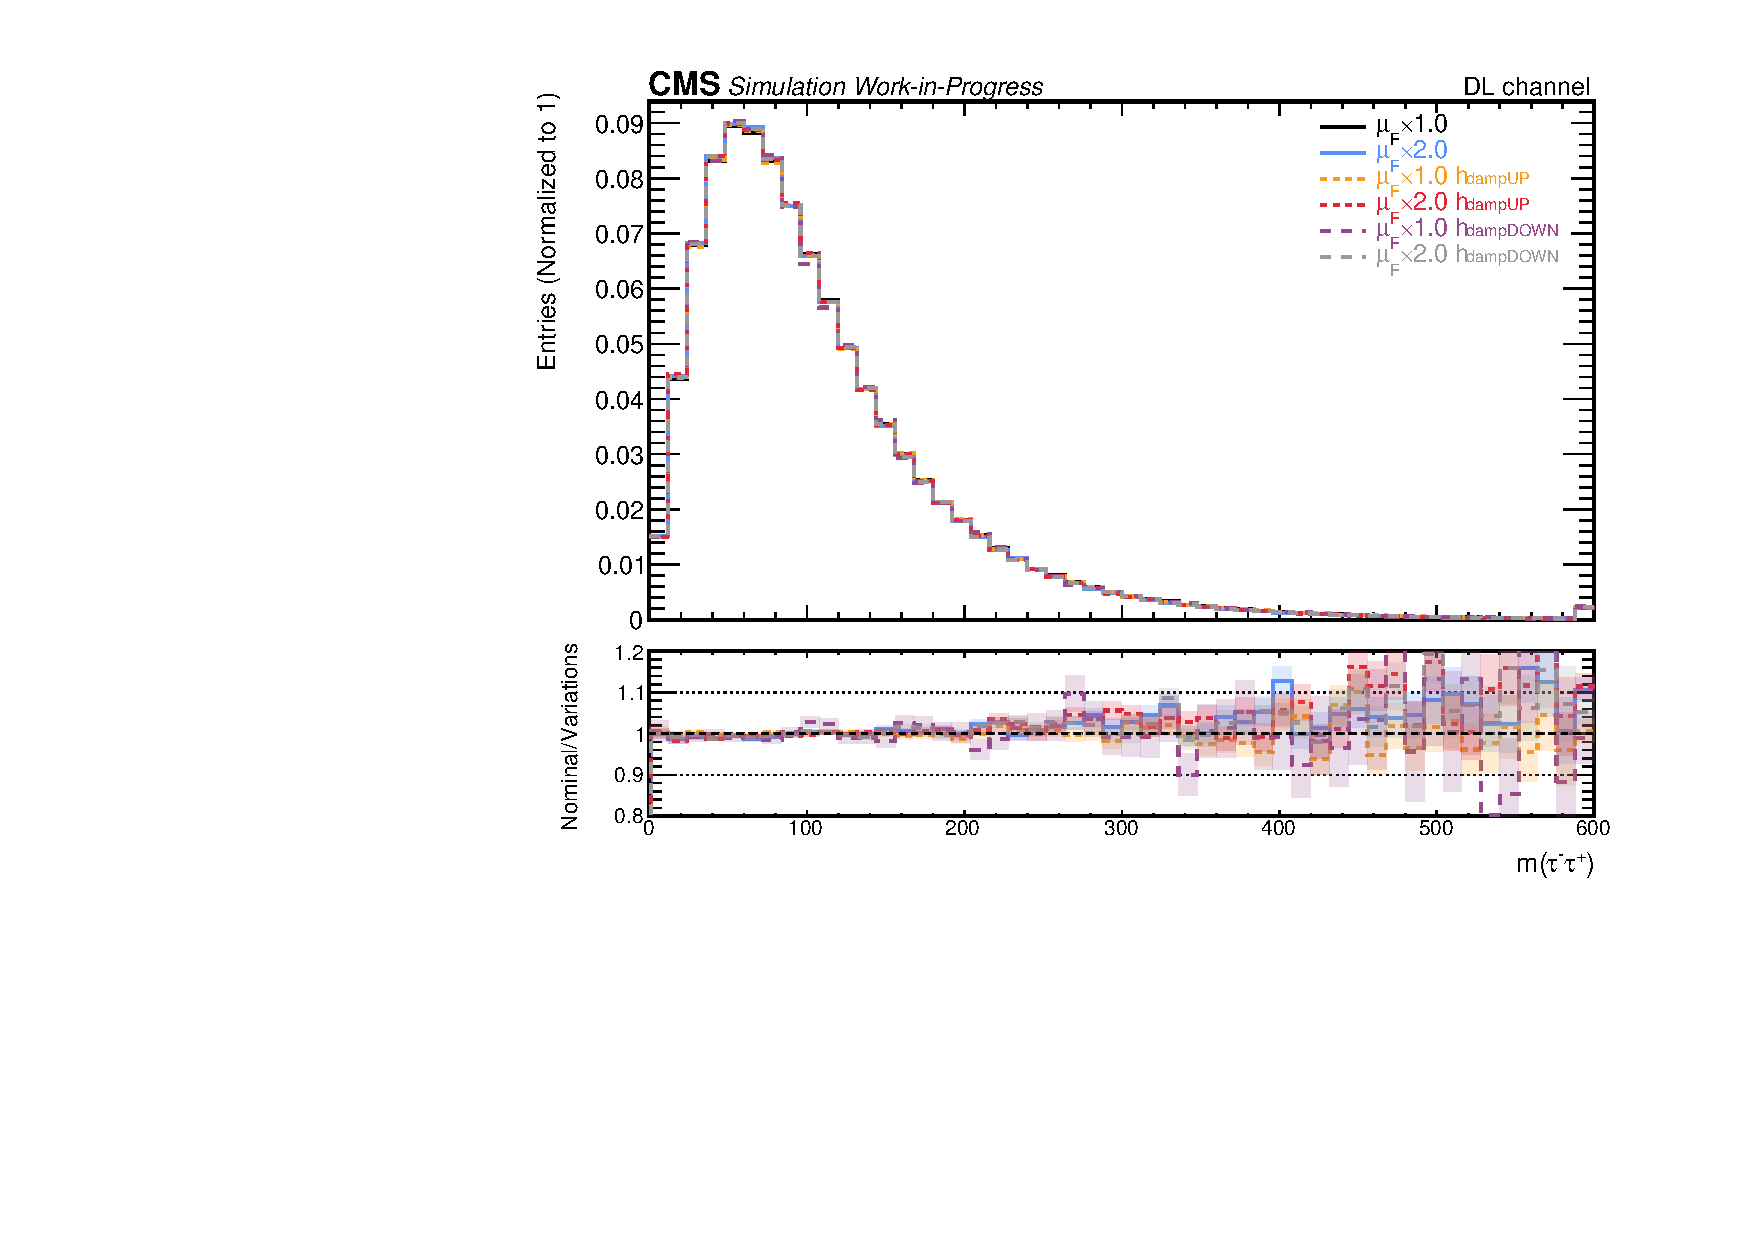
\includegraphics[width= 1.1\linewidth]{DL/ratio_tautau_system_invariant_mass.pdf}
        \caption{}
        \label{app:subfig:m(tt)_DL}
    \end{subfigure}

    \vspace{0.2cm}
    
    \begin{subfigure}{0.49\textwidth}
        \centering
        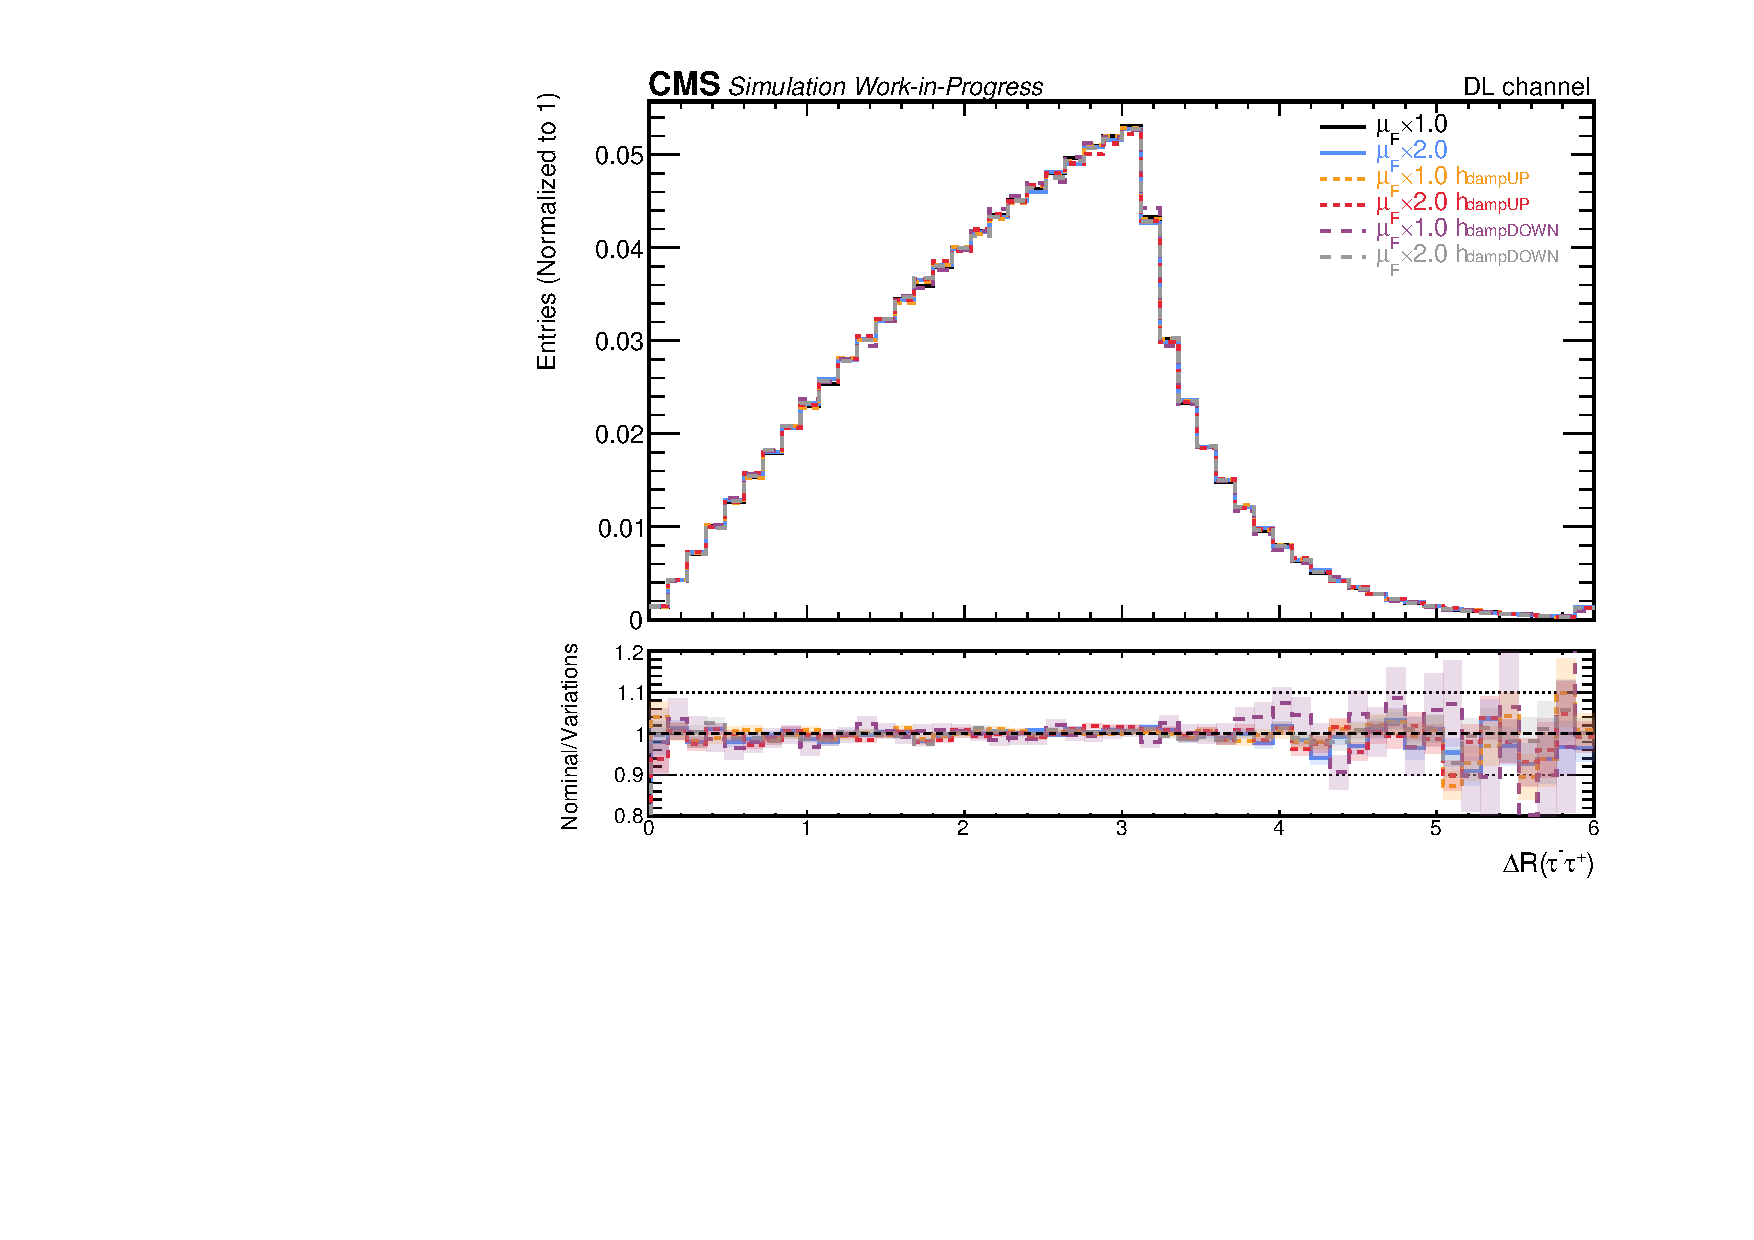
\includegraphics[width= 1.1\linewidth]{DL/ratio_tautau_system_dR.pdf}
        \caption{}
        \label{app:subfig:dR(tt)_DL}
    \end{subfigure}
    \begin{subfigure}{0.49\textwidth}
        \centering
        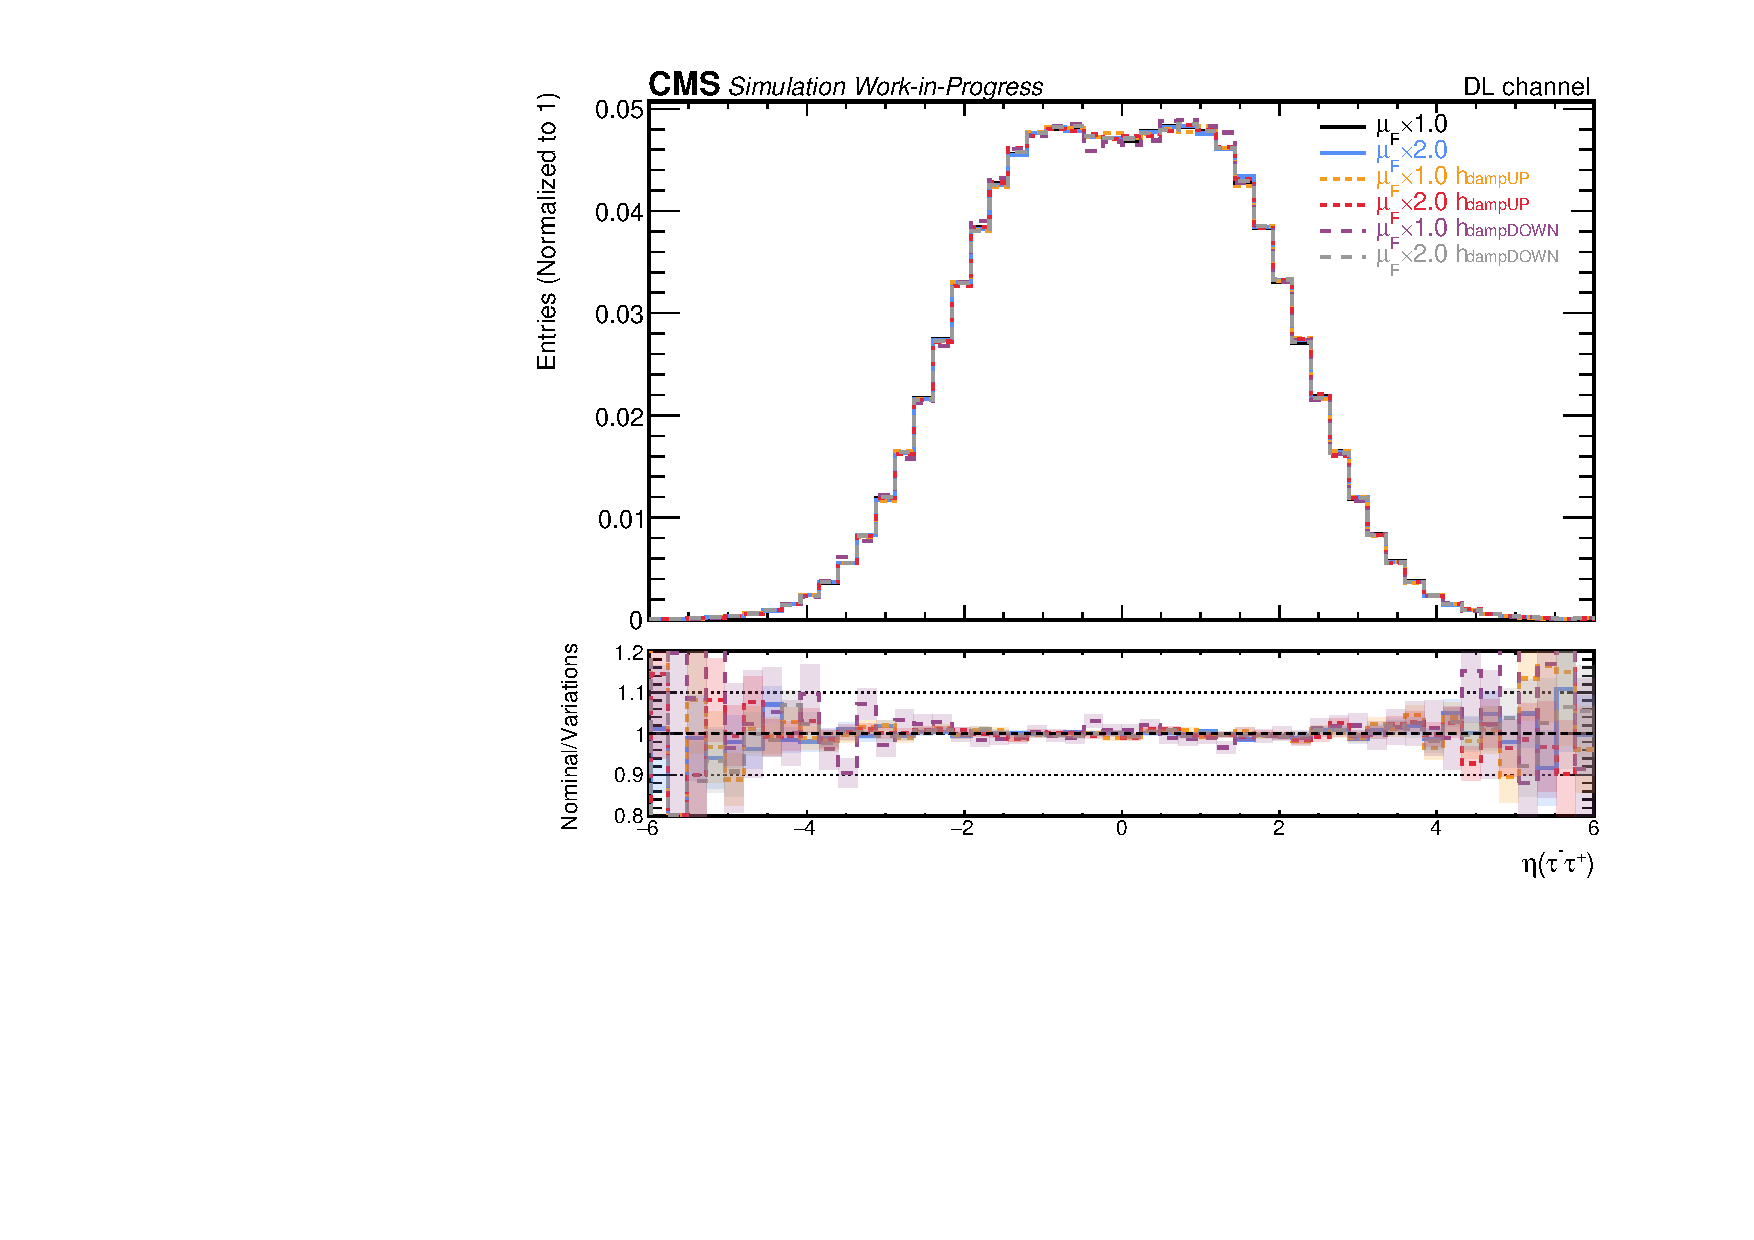
\includegraphics[width= 1.1\linewidth]{DL/ratio_tautau_system_pseudorapidity.pdf}
        \caption{}
        \label{app:subfig:eta(tt)_DL}
    \end{subfigure}
    \caption{Distributions of (a) transverse momentum, (b) invariant mass,  (c) angular separation and (d) rapidity of the $\tau^-\tau^+$ system for the six different settings used in the simulation. The lower panel shows the ratio of the nominal setting to the variations. The shaded bands represent statistical uncertainties. The last bins contain the overflow events.}
    \label{app:fig:tautau_DL}
\end{figure}


\begin{figure}[H]
    \centering
    \begin{subfigure}{0.49\textwidth}
        \centering
        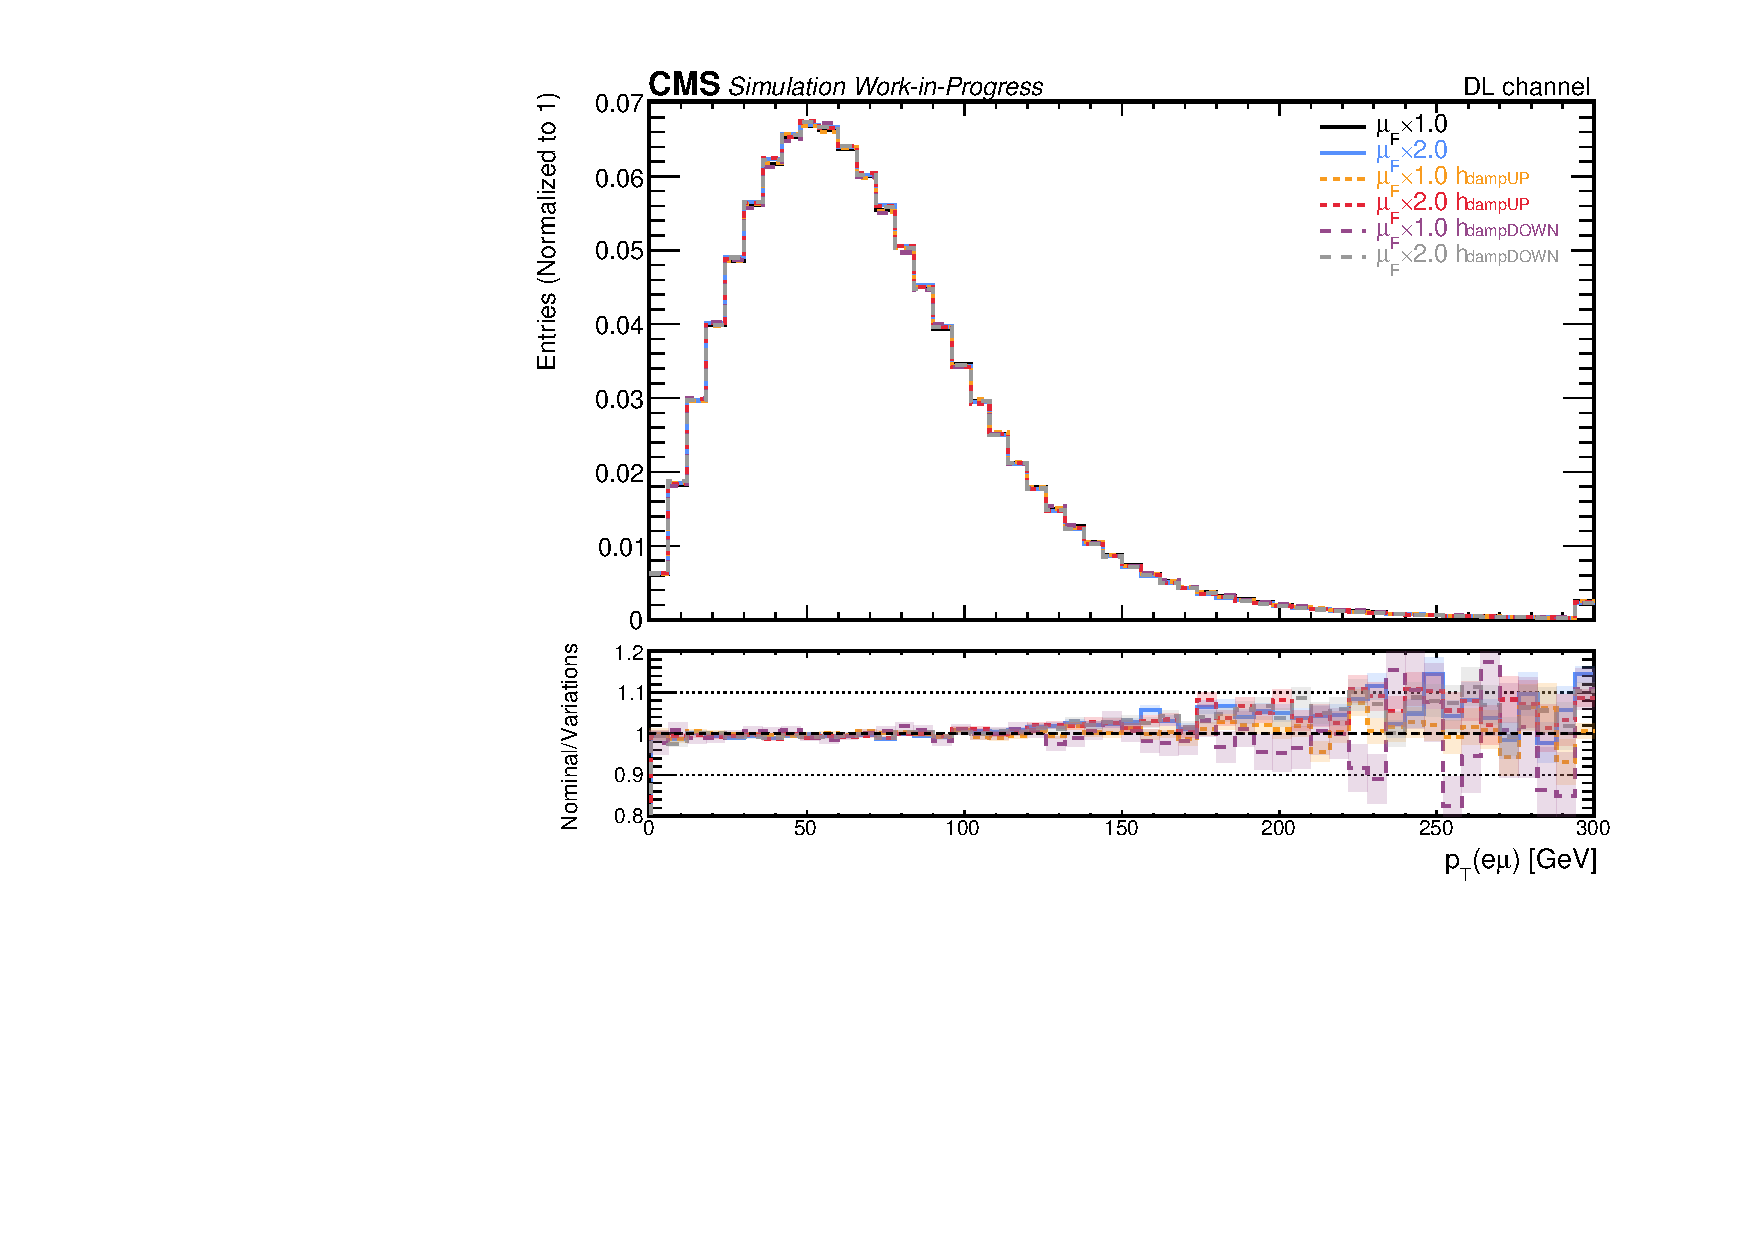
\includegraphics[width= 1.1\linewidth]{DL/ratio_em_system_pt.pdf}
        \caption{}
        \label{app:subfig:pt(em)_DL}
    \end{subfigure}
    \begin{subfigure}{0.49\textwidth}
        \centering
        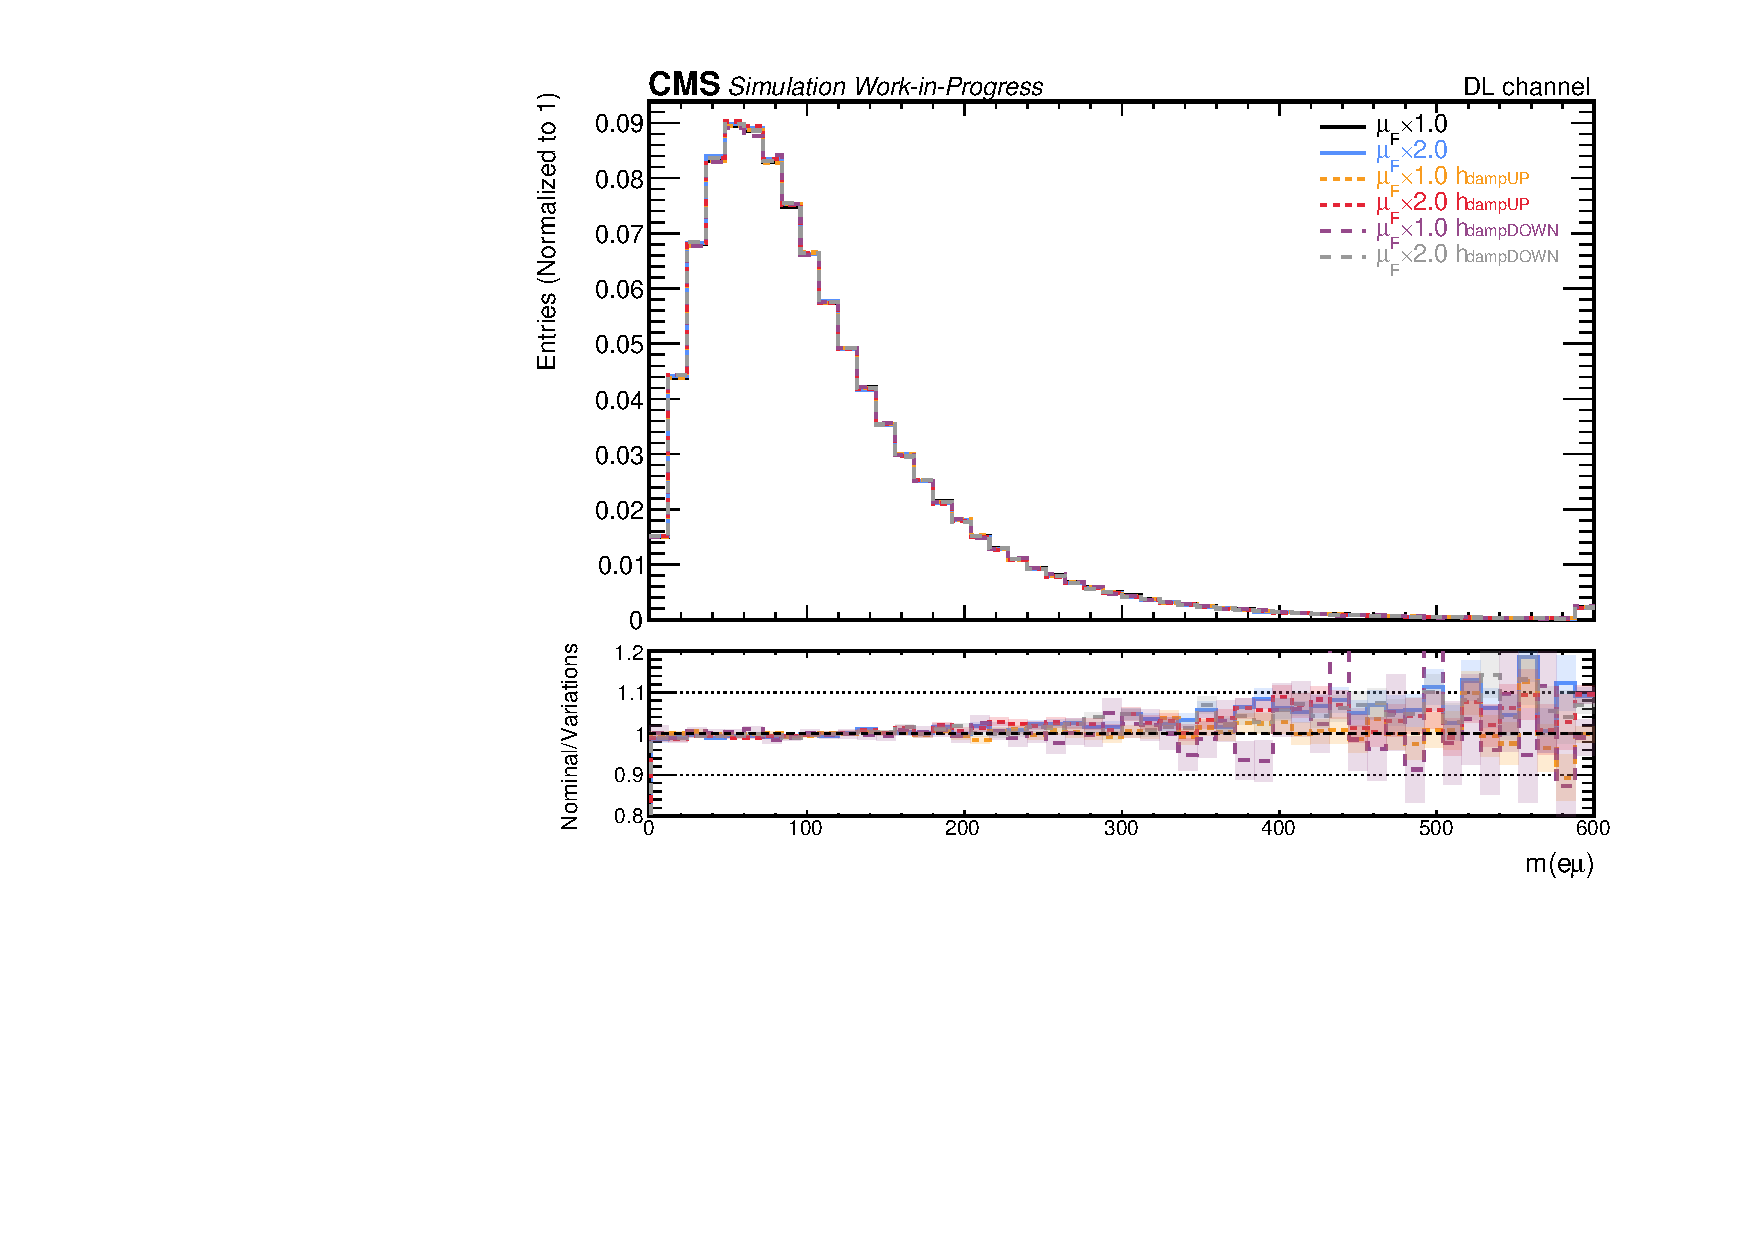
\includegraphics[width= 1.1\linewidth]{DL/ratio_em_system_invariant_mass.pdf}
        \caption{}
        \label{app:subfig:m(em)_DL}
    \end{subfigure}

    \vspace{0.2cm}
    
    \begin{subfigure}{0.49\textwidth}
        \centering
        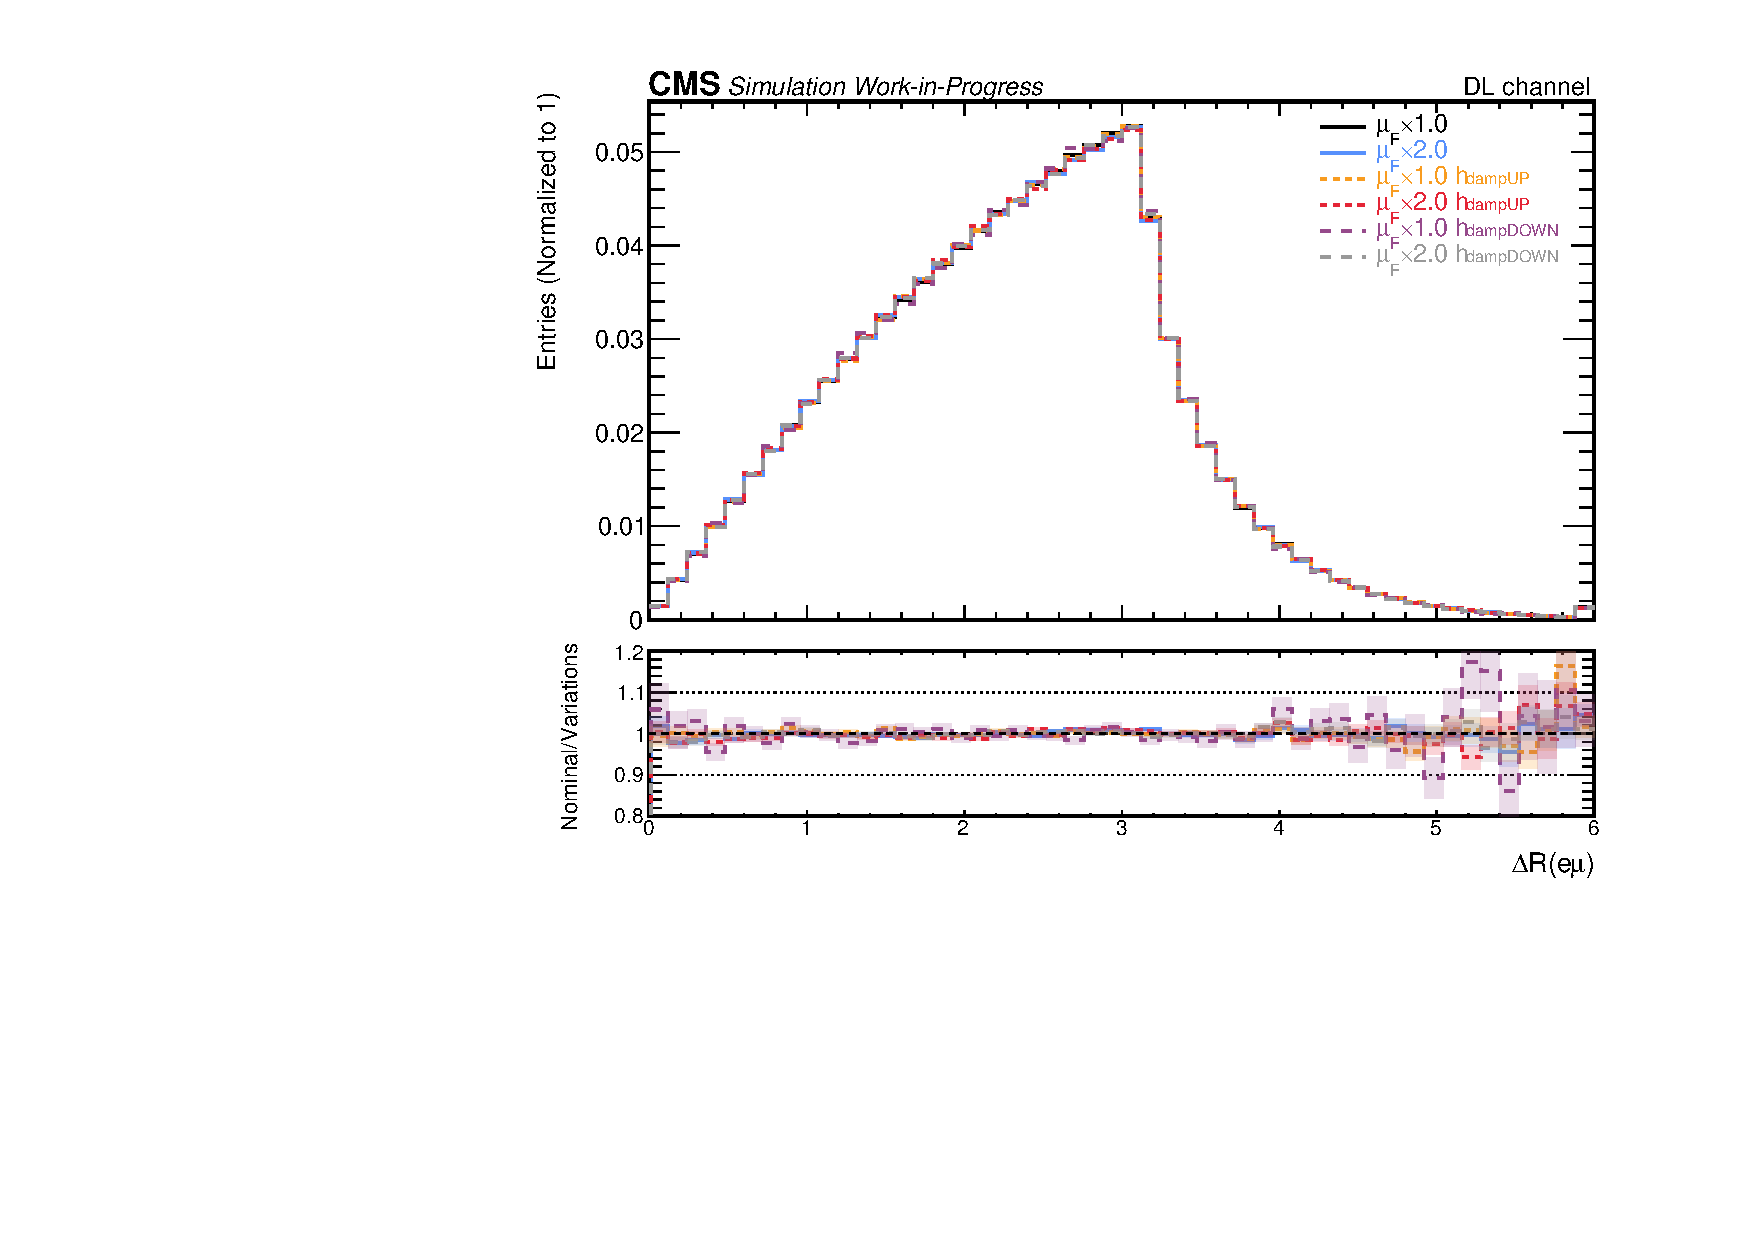
\includegraphics[width= 1.1\linewidth]{DL/ratio_em_system_dR.pdf}
        \caption{}
        \label{app:subfig:dR(em)_DL}
    \end{subfigure}
    \begin{subfigure}{0.49\textwidth}
        \centering
        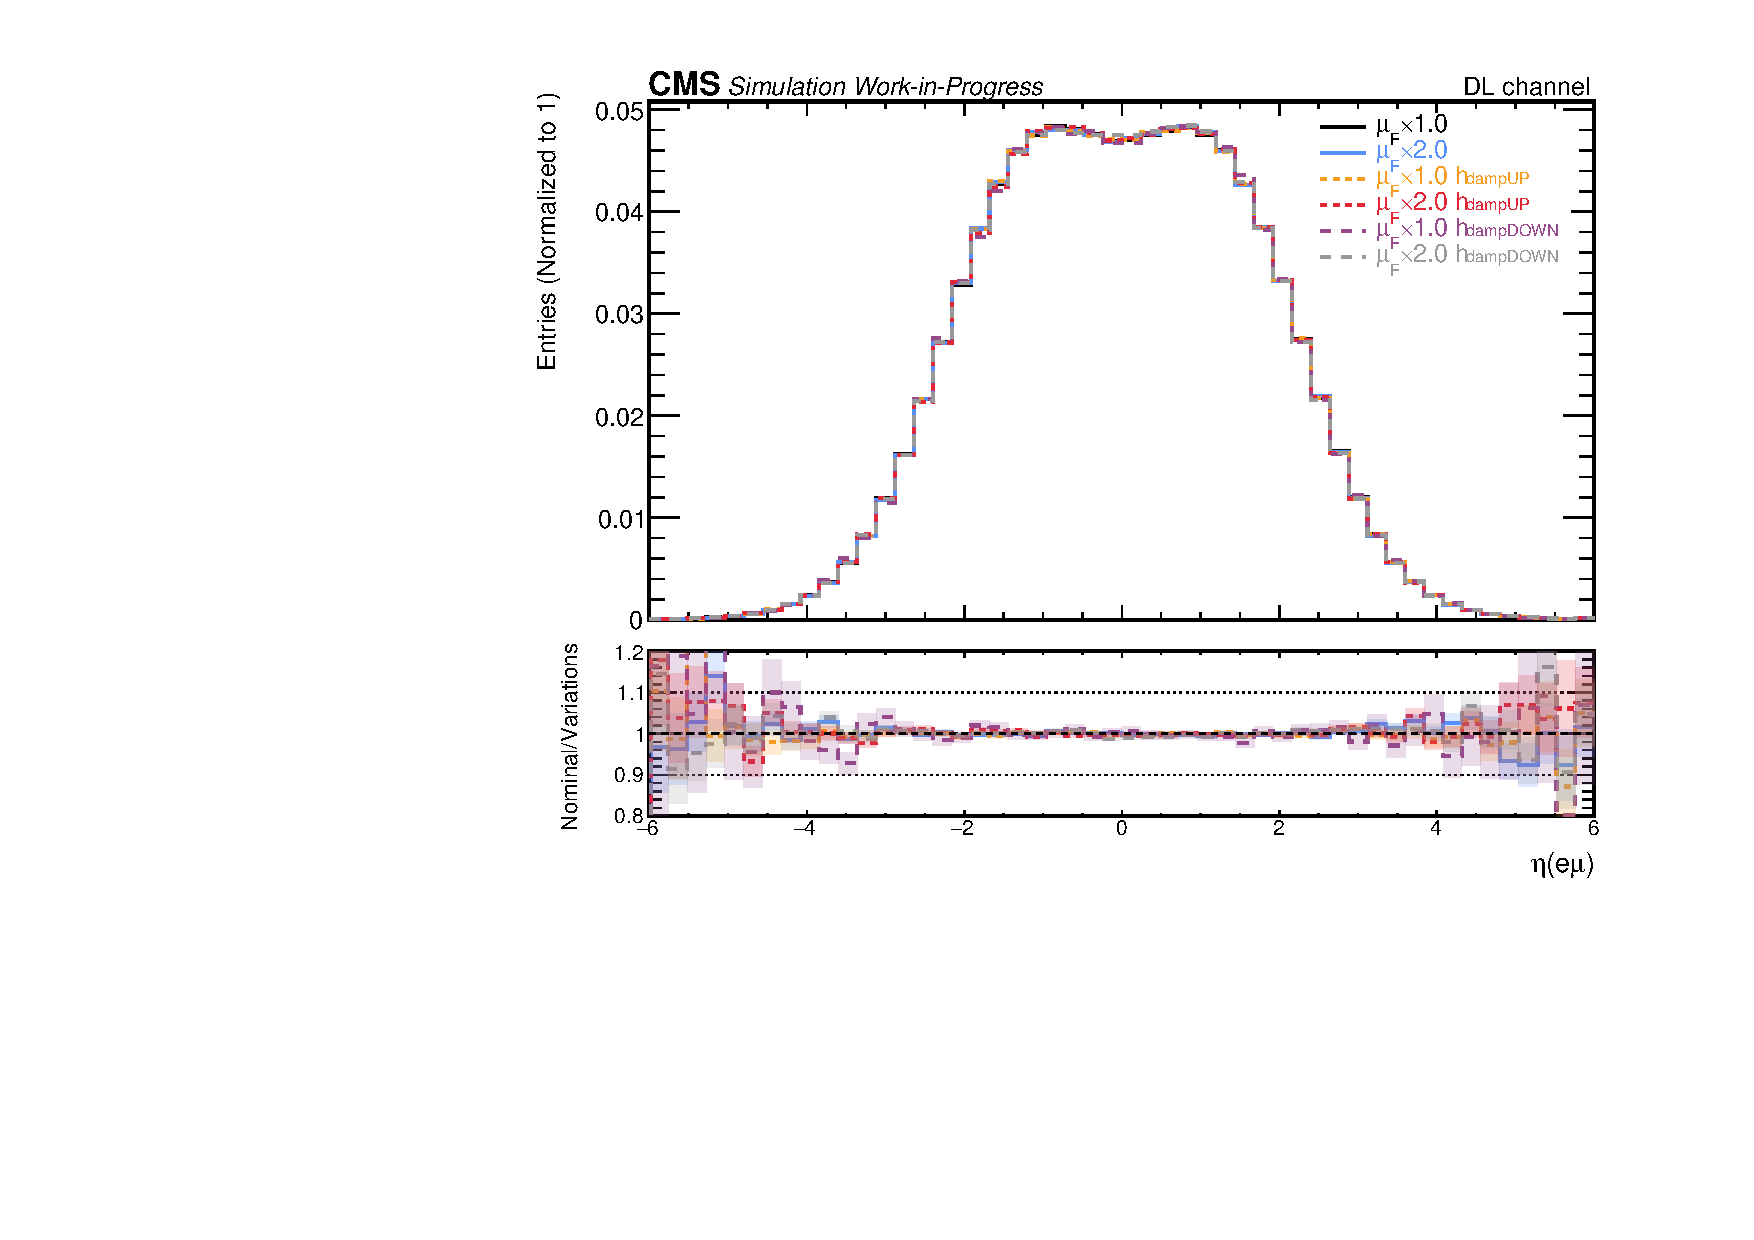
\includegraphics[width= 1.1\linewidth]{DL/ratio_em_system_pseudorapidity.pdf}
        \caption{}
        \label{app:subfig:eta(em)_DL}
    \end{subfigure}
    \caption{Distributions of (a) transverse momentum, (b) invariant mass,  (c) angular separation and (d) rapidity of the $e\mu$ system for the six different settings used in the simulation. The lower panel shows the ratio of the nominal setting to the variations. The shaded bands represent statistical uncertainties. The last bins contain the overflow events.}
    \label{app:fig:emu_DL}
\end{figure}


\begin{figure}[H]
    \centering
    \begin{subfigure}{0.49\textwidth}
        \centering
        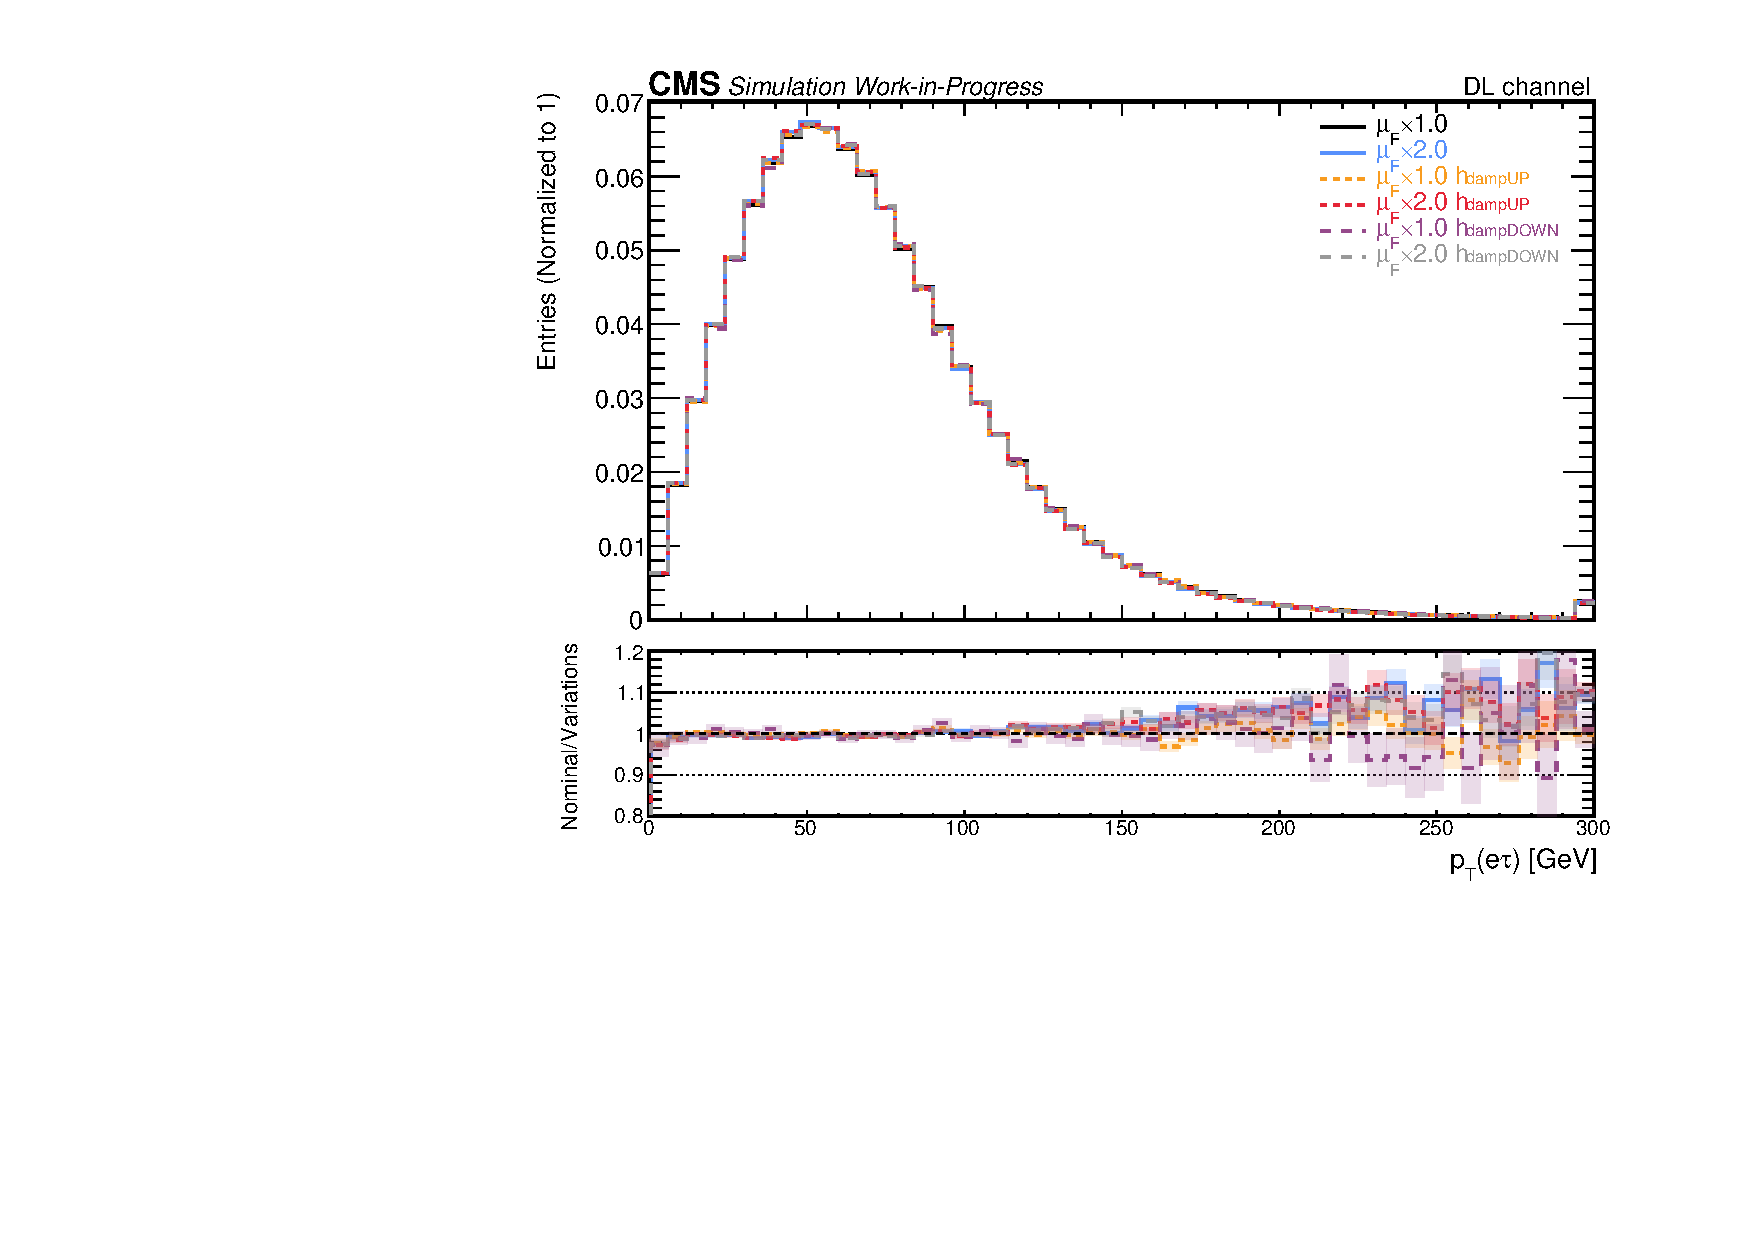
\includegraphics[width= 1.1\linewidth]{DL/ratio_et_system_pt.pdf}
        \caption{}
        \label{app:subfig:pt(et)_DL}
    \end{subfigure}
    \begin{subfigure}{0.49\textwidth}
        \centering
        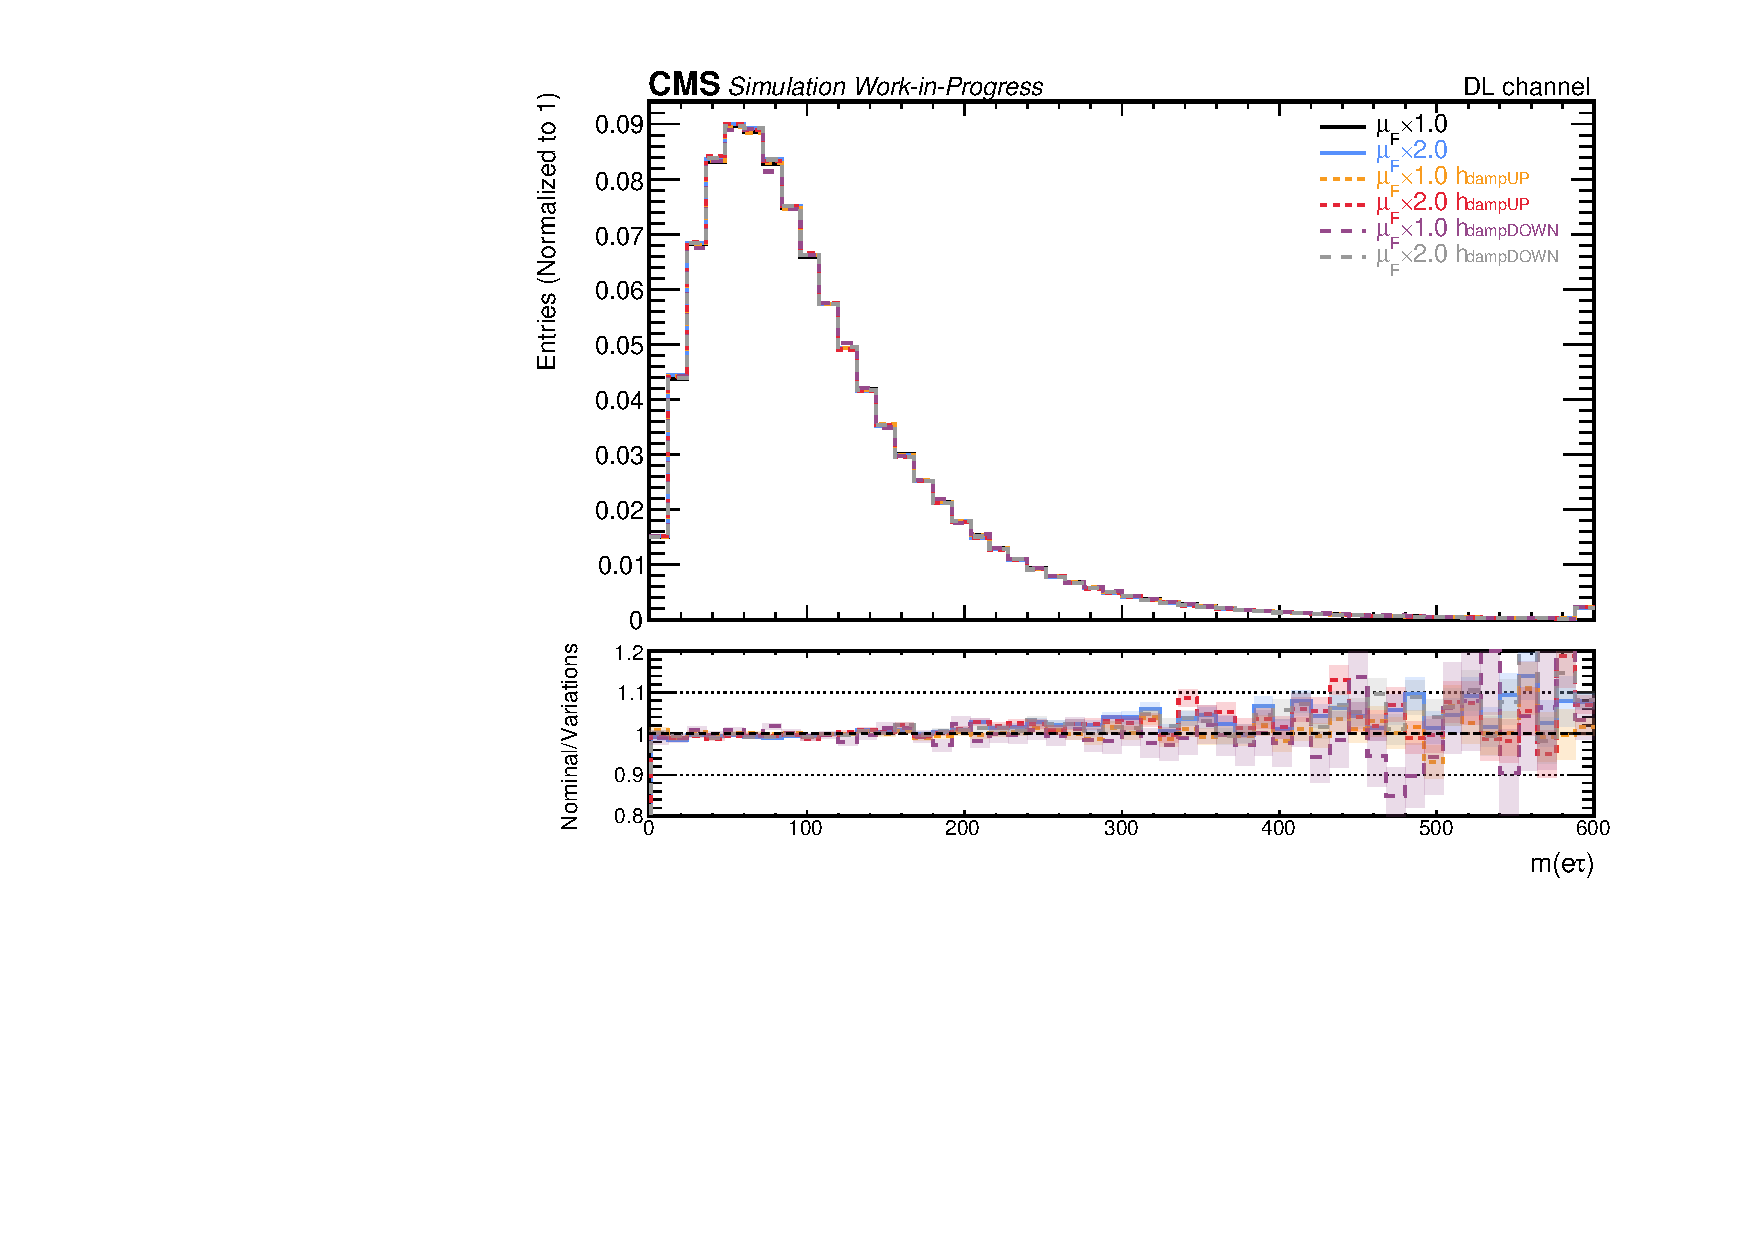
\includegraphics[width= 1.1\linewidth]{DL/ratio_et_system_invariant_mass.pdf}
        \caption{}
        \label{app:subfig:m(et)_DL}
    \end{subfigure}

    \vspace{0.2cm}
    
    \begin{subfigure}{0.49\textwidth}
        \centering
        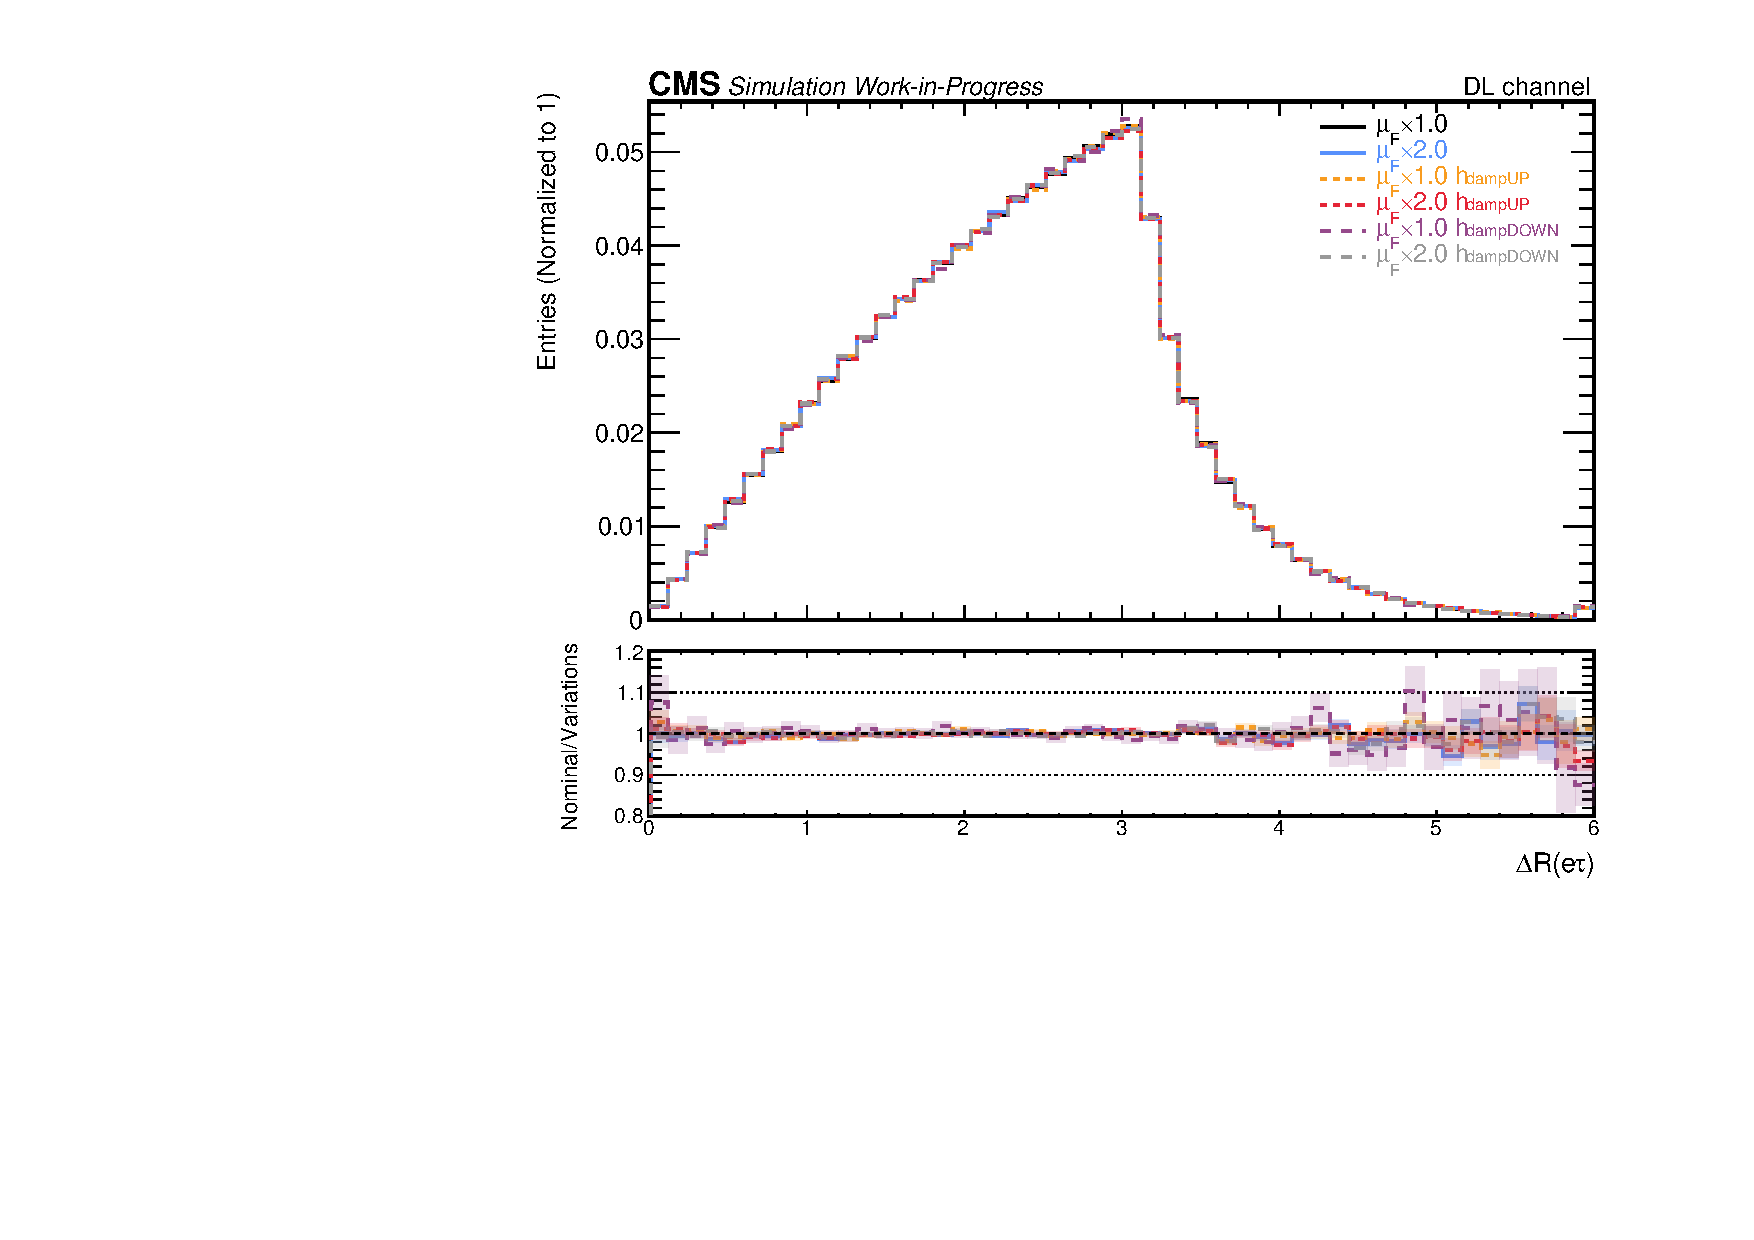
\includegraphics[width= 1.1\linewidth]{DL/ratio_et_system_dR.pdf}
        \caption{}
        \label{app:subfig:dR(et)_DL}
    \end{subfigure}
    \begin{subfigure}{0.49\textwidth}
        \centering
        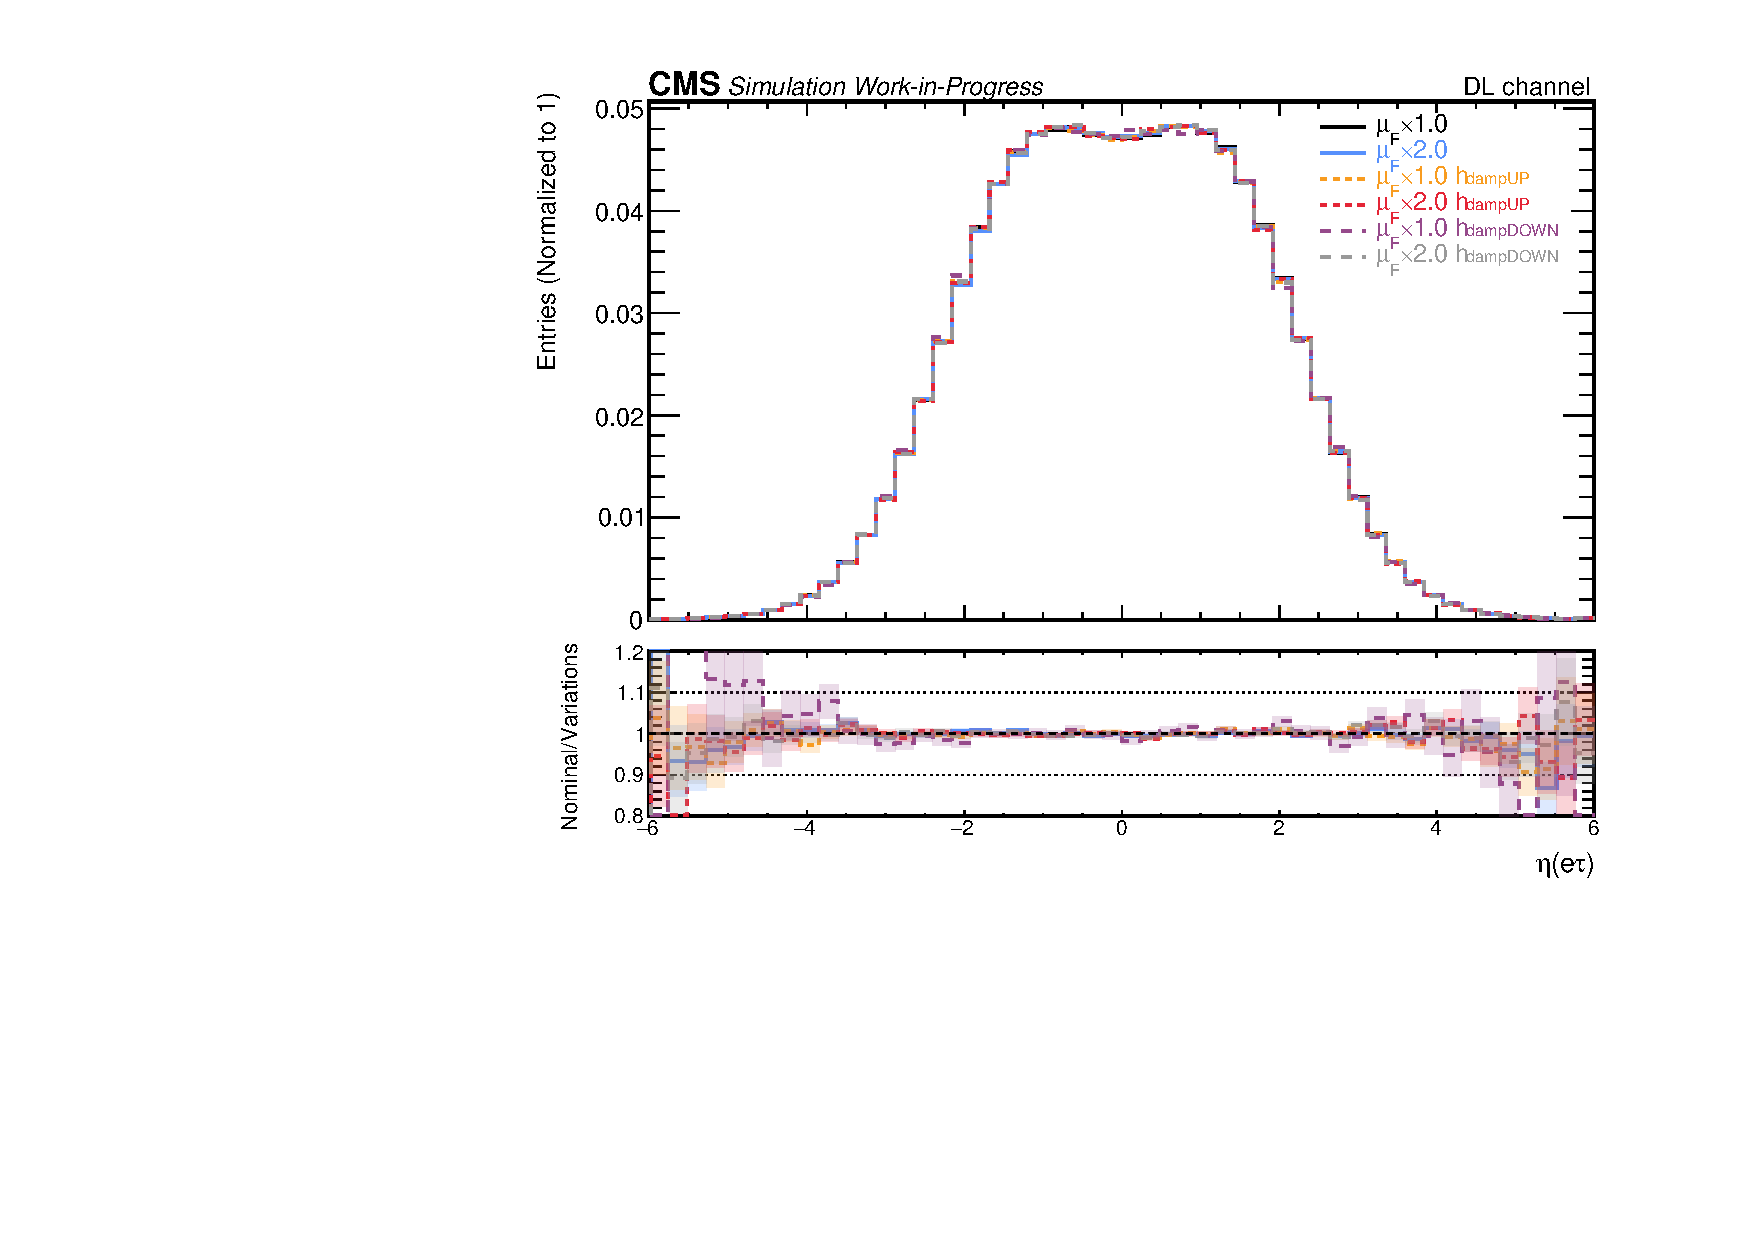
\includegraphics[width= 1.1\linewidth]{DL/ratio_et_system_pseudorapidity.pdf}
        \caption{}
        \label{app:subfig:eta(et)_DL}
    \end{subfigure}
    \caption{Distributions of (a) transverse momentum, (b) invariant mass,  (c) angular separation and (d) rapidity of the $e\tau$ system for the six different settings used in the simulation. The lower panel shows the ratio of the nominal setting to the variations. The shaded bands represent statistical uncertainties. The last bins contain the overflow events.}
    \label{app:fig:etau_DL}
\end{figure}


\begin{figure}[H]
    \centering
    \begin{subfigure}{0.49\textwidth}
        \centering
        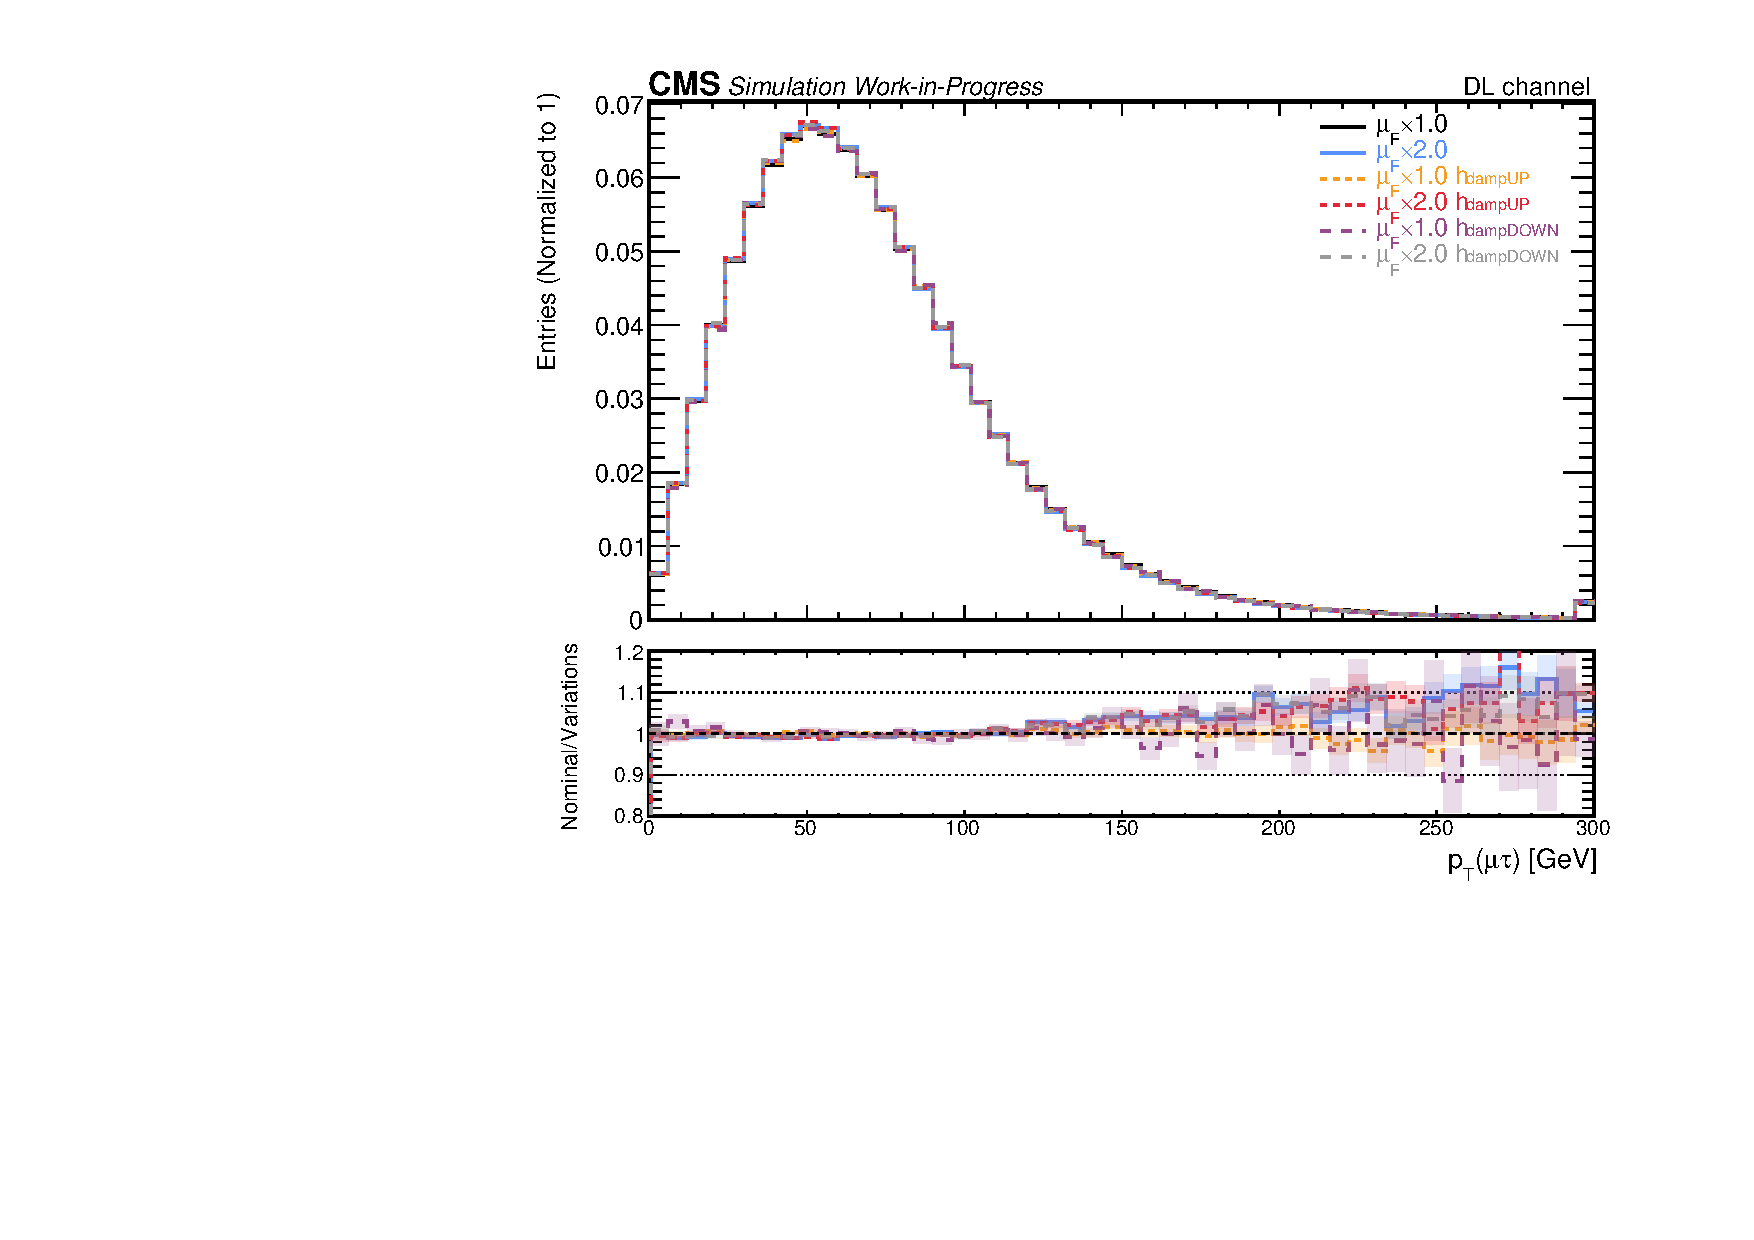
\includegraphics[width= 1.1\linewidth]{DL/ratio_mt_system_pt.pdf}
        \caption{}
        \label{app:subfig:pt(mt)_DL}
    \end{subfigure}
    \begin{subfigure}{0.49\textwidth}
        \centering
        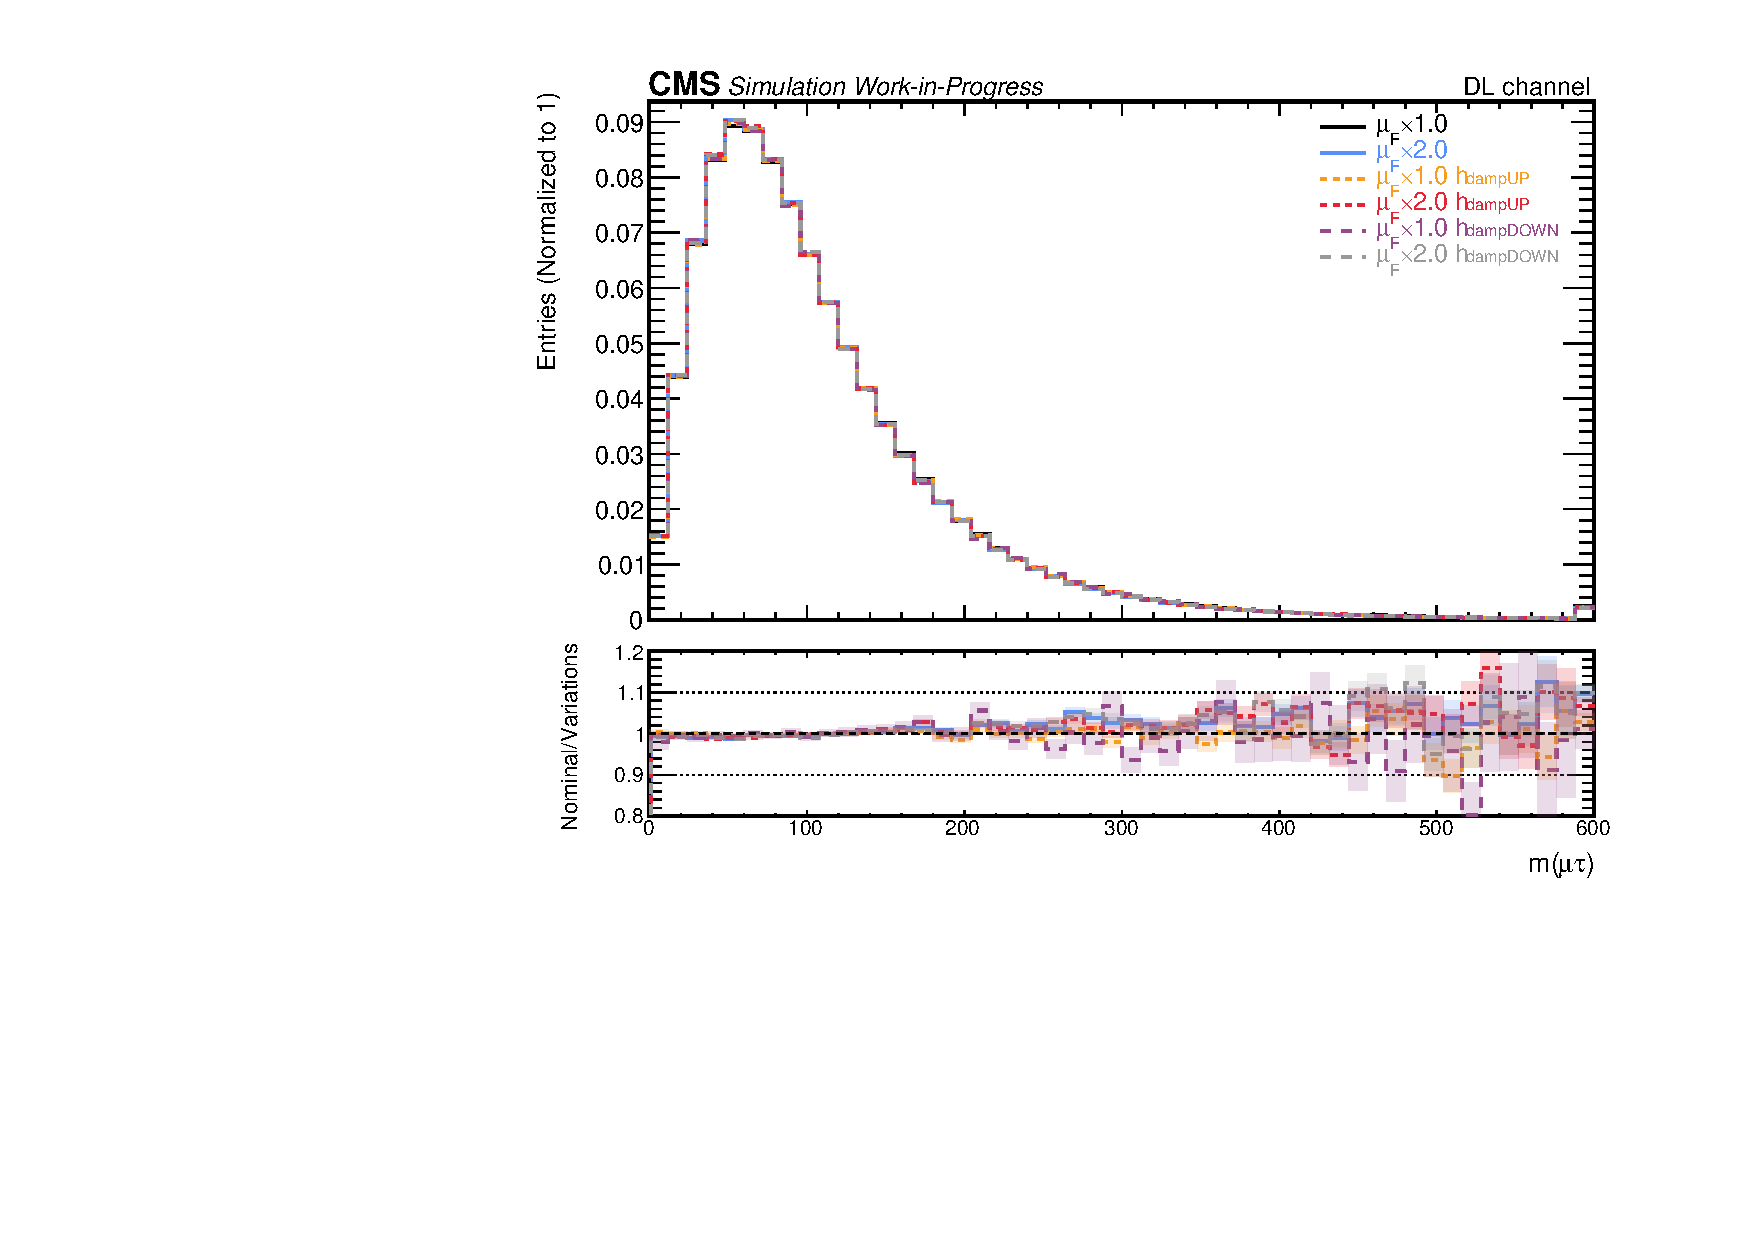
\includegraphics[width= 1.1\linewidth]{DL/ratio_mt_system_invariant_mass.pdf}
        \caption{}
        \label{app:subfig:m(mt)_DL}
    \end{subfigure}

    \vspace{0.2cm}
    
    \begin{subfigure}{0.49\textwidth}
        \centering
        \includegraphics[width= 1.1\linewidth]{DL/ratio_mt_system_dR.pdf}
        \caption{}
        \label{app:subfig:dR(mt)_DL}
    \end{subfigure}
    \begin{subfigure}{0.49\textwidth}
        \centering
        \includegraphics[width= 1.1\linewidth]{DL/ratio_mt_system_pseudorapidity.pdf}
        \caption{}
        \label{app:subfig:eta(mt)_DL}
    \end{subfigure}
    \caption{Distributions of (a) transverse momentum, (b) invariant mass,  (c) angular separation and (d) rapidity of the $\mu\tau$ system for the six different settings used in the simulation. The lower panel shows the ratio of the nominal setting to the variations. The shaded bands represent statistical uncertainties. The last bins contain the overflow events.}
    \label{app:fig:mutau_DL}
\end{figure}


\begin{figure}[H]
    \centering
    \begin{subfigure}{0.49\textwidth}
        \centering
        \includegraphics[width= 1.1\linewidth]{DL/ratio_radiation_energy.pdf}
        \caption{}
        \label{app:subfig:E(radiation)_DL}
    \end{subfigure}
    \begin{subfigure}{0.49\textwidth}
        \centering
        \includegraphics[width= 1.1\linewidth]{DL/ratio_radiation_pt.pdf}
        \caption{}
        \label{app:subfig:pt(radiation)_DL}
    \end{subfigure}

    \vspace{0.2cm}
    
    \begin{subfigure}{0.49\textwidth}
        \centering
        \includegraphics[width= 1.1\linewidth]{DL/ratio_radiation_phi.pdf}
        \caption{}
        \label{app:subfig:phi(radiation)_DL}
    \end{subfigure}
    \begin{subfigure}{0.49\textwidth}
        \centering
        \includegraphics[width= 1.1\linewidth]{DL/ratio_radiation_pseudorapidity.pdf}
        \caption{}
        \label{app:subfig:eta(radiation)_DL}
    \end{subfigure}
    \caption{Distributions of (a) energy, (b) transverse momentum,  (c) azimuthal angle and (d) pseudorapidity of the extra light jet for the six different settings used in the simulation. The lower panel shows the ratio of the nominal setting to the variations. The shaded bands represent statistical uncertainties. The last bins contain the overflow events.}
    \label{app:fig:radiation_DL}
\end{figure}


\section{\label{app:SL}SL channel}

\begin{figure}[H]
    \centering
    \begin{subfigure}{0.49\textwidth}
        \centering
        \includegraphics[width= 1.1\linewidth]{SL/ratio_ttbar_energy.pdf}
        \caption{}
        \label{app:subfig:E(t,tbar)_SL}
    \end{subfigure}
    \begin{subfigure}{0.48\textwidth}
        \centering
        \includegraphics[width= 1.1\linewidth]{SL/ratio_ttbar_reco_mass.pdf}
        \caption{}
        \label{app:subfig:m(t,tbar)_SL}
    \end{subfigure}

    \vspace{0.2cm}
    
    \begin{subfigure}{0.49\textwidth}
        \centering
        \includegraphics[width= 1.1\linewidth]{SL/ratio_ttbar_phi.pdf}
        \caption{}
        \label{app:subfig:phi(t,tbar)_SL}
    \end{subfigure}
    \begin{subfigure}{0.49\textwidth}
        \centering
        \includegraphics[width= 1.1\linewidth]{SL/ratio_ttbar_rapidity.pdf}
        \caption{}
        \label{app:subfig:y(t,tbar)_SL}
    \end{subfigure}
    
    \caption{Distributions of (a) energy, (b) reconstructed mass,  (c) azimuthal angle and (d) rapidity of the t/$\overline{\text{t}}$ quarks for the six different settings used in the simulation. The lower panel shows the ratio of the nominal setting to the variations. The shaded bands represent statistical uncertainties. The last bins contain the overflow events.}
    \label{app:fig:t,tbar_SL}
\end{figure}


\begin{figure}[H]
    \centering
    \begin{subfigure}{0.49\textwidth}
        \centering
        \includegraphics[width= 1.1\linewidth]{SL/ratio_tt_system_pt.pdf}
        \caption{}
        \label{app:subfig:pt(ttbar)_SL}
    \end{subfigure}
    \begin{subfigure}{0.49\textwidth}
        \centering
        \includegraphics[width= 1.1\linewidth]{SL/ratio_tt_system_invariant_mass.pdf}
        \caption{}
        \label{app:subfig:m(ttbar_SL}
    \end{subfigure}

    \vspace{0.2cm}
    
    \begin{subfigure}{0.49\textwidth}
        \centering
        \includegraphics[width= 1.1\linewidth]{SL/ratio_tt_system_dR.pdf}
        \caption{}
        \label{app:subfig:dR(ttbar)_SL}
    \end{subfigure}
    \begin{subfigure}{0.49\textwidth}
        \centering
        \includegraphics[width= 1.1\linewidth]{SL/ratio_tt_system_rapidity.pdf}
        \caption{}
        \label{app:subfig:y(ttbar)_SL}
    \end{subfigure}
    \caption{Distributions of (a) transverse momentum, (b) invariant mass,  (c) angular separation and (d) rapidity of the t$\overline{\text{t}}$ system for the six different settings used in the simulation. The lower panel shows the ratio of the nominal setting to the variations. The shaded bands represent statistical uncertainties. The last bins contain the overflow events.}
    \label{app:fig:ttbar_SL}
\end{figure}


\begin{figure}[H]
    \centering
    \begin{subfigure}{0.49\textwidth}
        \centering
        \includegraphics[width= 1.1\linewidth]{SL/ratio_b_all_energy.pdf}
        \caption{}
        \label{app:subfig:Ε(b_all)_SL}
    \end{subfigure}
    \begin{subfigure}{0.49\textwidth}
        \centering
        \includegraphics[width= 1.1\linewidth]{SL/ratio_b_all_pt.pdf}
        \caption{}
        \label{app:subfig:pt(b_all)_SL}
    \end{subfigure}

    \vspace{0.2cm}
    
    \begin{subfigure}{0.49\textwidth}
        \centering
        \includegraphics[width= 1.1\linewidth]{SL/ratio_b_all_phi.pdf}
        \caption{}
        \label{app:subfig:phi(b_all)_SL}
    \end{subfigure}
    \begin{subfigure}{0.49\textwidth}
        \centering
        \includegraphics[width= 1.1\linewidth]{SL/ratio_b_all_pseudorapidity.pdf}
        \caption{}
        \label{app:subfig:eta(b_all)_SL}
    \end{subfigure}
    \caption{Distributions of (a) energy, (b) transverse momentum,  (c) azimuthal angle and (d) pseudorapidity of all the b/$\overline{\text{b}}$ quarks for the six different settings used in the simulation. The lower panel shows the ratio of the nominal setting to the variations. The shaded bands represent statistical uncertainties. The last bins contain the overflow events.}
    \label{app:fig:b_all_SL}
\end{figure}



\begin{figure}[H]
    \centering
    \begin{subfigure}{0.49\textwidth}
        \centering
        \includegraphics[width= 1.1\linewidth]{SL/ratio_bs_from_top_pt.pdf}
        \caption{}
        \label{app:subfig:pt(bbbar)_SL}
    \end{subfigure}
    \begin{subfigure}{0.49\textwidth}
        \centering
        \includegraphics[width= 1.1\linewidth]{SL/ratio_bs_from_top_invariant_mass.pdf}
        \caption{}
        \label{app:subfig:m(bbbar)_SL}
    \end{subfigure}

    \vspace{0.2cm}
    
    \begin{subfigure}{0.49\textwidth}
        \centering
        \includegraphics[width= 1.1\linewidth]{SL/ratio_bs_from_top_dR.pdf}
        \caption{}
        \label{app:subfig:dR(bbbar)_SL}
    \end{subfigure}
    \begin{subfigure}{0.49\textwidth}
        \centering
        \includegraphics[width= 1.1\linewidth]{SL/ratio_bs_from_top_rapidity.pdf}
        \caption{}
        \label{app:subfig:y(bbbar)_SL}
    \end{subfigure}
    \caption{Distributions of (a) transverse momentum, (b) invariant mass,  (c) angular separation and (d) rapidity of the b$\overline{\text{b}}$ system, related to top quarks, for the six different settings used in the simulation. The lower panel shows the ratio of the nominal setting to the variations. The shaded bands represent statistical uncertainties. The last bins contain the overflow events.}
    \label{app:fig:bbbar_SL}
\end{figure}

\begin{figure}[H]
    \centering
    \begin{subfigure}{0.49\textwidth}
        \centering
        \includegraphics[width= 1.1\linewidth]{SL/ratio_prompt_bs_pt.pdf}
        \caption{}
        \label{app:subfig:pt(bbbar_prompt)_SL}
    \end{subfigure}
    \begin{subfigure}{0.49\textwidth}
        \centering
        \includegraphics[width= 1.1\linewidth]{SL/ratio_prompt_bs_invariant_mass.pdf}
        \caption{}
        \label{app:subfig:m(bbbar_prompt)_SL}
    \end{subfigure}

    \vspace{0.2cm}
    
    \begin{subfigure}{0.49\textwidth}
        \centering
        \includegraphics[width= 1.1\linewidth]{SL/ratio_prompt_bs_dR.pdf}
        \caption{}
        \label{app:subfig:dR(bbbar_prompt)_SL}
    \end{subfigure}
    \begin{subfigure}{0.49\textwidth}
        \centering
        \includegraphics[width= 1.1\linewidth]{SL/ratio_prompt_bs_rapidity.pdf}
        \caption{}
        \label{app:subfig:y(bbbar_prompt)_SL}
    \end{subfigure}
    \caption{Distributions of (a) transverse momentum, (b) invariant mass,  (c) angular separation and (d) rapidity of the prompt b$\overline{\text{b}}$ system for the six different settings used in the simulation. The lower panel shows the ratio of the nominal setting to the variations. The shaded bands represent statistical uncertainties. The last bins contain the overflow events.}
    \label{app:fig:prompt_bbbar_SL}
\end{figure}


\begin{figure}[H]
    \centering
    \begin{subfigure}{0.49\textwidth}
        \centering
        \includegraphics[width= 1.1\linewidth]{SL/ratio_leptons_energy.pdf}
        \caption{}
        \label{app:subfig:E(leptons)_SL}
    \end{subfigure}
    \begin{subfigure}{0.49\textwidth}
        \centering
        \includegraphics[width= 1.1\linewidth]{SL/ratio_leptons_pt.pdf}
        \caption{}
        \label{app:subfig:pt(leptons)_SL}
    \end{subfigure}

    \vspace{0.2cm}
    
    \begin{subfigure}{0.49\textwidth}
        \centering
        \includegraphics[width= 1.1\linewidth]{SL/ratio_leptons_phi.pdf}
        \caption{}
        \label{app:subfig:phi(leptons)_SL}
    \end{subfigure}
    \begin{subfigure}{0.49\textwidth}
        \centering
        \includegraphics[width= 1.1\linewidth]{SL/ratio_leptons_pseudorapidity.pdf}
        \caption{}
        \label{app:subfig:eta(leptons)_SL}
    \end{subfigure}
    \caption{Distributions of (a) energy, (b) transverse momentum,  (c) azimuthal angle and (d) pseudorapidity of all the leptons (charged and neutral) for the six different settings used in the simulation. The lower panel shows the ratio of the nominal setting to the variations. The shaded bands represent statistical uncertainties. The last bins contain the overflow events.}
    \label{app:fig:leptons_SL}
\end{figure}




\begin{figure}[H]
    \centering
    \begin{subfigure}{0.49\textwidth}
        \centering
        \includegraphics[width= 1.1\linewidth]{SL/ratio_quarks_energy.pdf}
        \caption{}
        \label{app:subfig:E(quarks)_SL}
    \end{subfigure}
    \begin{subfigure}{0.49\textwidth}
        \centering
        \includegraphics[width= 1.1\linewidth]{SL/ratio_quarks_pt.pdf}
        \caption{}
        \label{app:subfig:pt(quarks)_SL}
    \end{subfigure}

    \vspace{0.2cm}
    
    \begin{subfigure}{0.49\textwidth}
        \centering
        \includegraphics[width= 1.1\linewidth]{SL/ratio_quarks_phi.pdf}
        \caption{}
        \label{app:subfig:phi(quarks)_SL}
    \end{subfigure}
    \begin{subfigure}{0.49\textwidth}
        \centering
        \includegraphics[width= 1.1\linewidth]{SL/ratio_quarks_pseudorapidity.pdf}
        \caption{}
        \label{app:subfig:eta(quarks)_SL}
    \end{subfigure}
    \caption{Distributions of (a) energy, (b) transverse momentum,  (c) azimuthal angle and (d) pseudorapidity of the light flavor quarks, related to W bosons, for the six different settings used in the simulation. The lower panel shows the ratio of the nominal setting to the variations. The shaded bands represent statistical uncertainties. The last bins contain the overflow events.}
    \label{app:fig:quarks_SL}
\end{figure}

\begin{figure}[H]
    \centering
    \begin{subfigure}{0.49\textwidth}
        \centering
        \includegraphics[width= 1.1\linewidth]{SL/ratio_quarks_system_pt.pdf}
        \caption{}
        \label{app:subfig:pt(qq)_SL}
    \end{subfigure}
    \begin{subfigure}{0.49\textwidth}
        \centering
        \includegraphics[width= 1.1\linewidth]{SL/ratio_quarks_system_invariant_mass.pdf}
        \caption{}
        \label{app:subfig:m(qq)_SL}
    \end{subfigure}

    \vspace{0.2cm}
    
    \begin{subfigure}{0.49\textwidth}
        \centering
        \includegraphics[width= 1.1\linewidth]{SL/ratio_quarks_system_dR.pdf}
        \caption{}
        \label{app:subfig:dR(qq)_SL}
    \end{subfigure}
    \begin{subfigure}{0.49\textwidth}
        \centering
        \includegraphics[width= 1.1\linewidth]{SL/ratio_quarks_system_pseudorapidity.pdf}
        \caption{}
        \label{app:subfig:y(qq)_SL}
    \end{subfigure}
    \caption{Distributions of (a) transverse momentum, (b) invariant mass,  (c) angular separation and (d) rapidity of the $\overline{\text{q}}$q' system for the six different settings used in the simulation. The lower panel shows the ratio of the nominal setting to the variations. The shaded bands represent statistical uncertainties. The last bins contain the overflow events.}
    \label{app:fig:qqbar_SL}
\end{figure}



\begin{figure}[H]
    \centering
    \begin{subfigure}{0.49\textwidth}
        \centering
        \includegraphics[width= 1.1\linewidth]{SL/ratio_ud_pairs_system_pt.pdf}
        \caption{}
        \label{app:subfig:pt(ud)_SL}
    \end{subfigure}
    \begin{subfigure}{0.49\textwidth}
        \centering
        \includegraphics[width= 1.1\linewidth]{SL/ratio_ud_pairs_system_invariant_mass.pdf}
        \caption{}
        \label{app:subfig:m(ud)_SL}
    \end{subfigure}

    \vspace{0.2cm}
    
    \begin{subfigure}{0.49\textwidth}
        \centering
        \includegraphics[width= 1.1\linewidth]{SL/ratio_ud_pairs_system_dR.pdf}
        \caption{}
        \label{app:subfig:dR(ud)_SL}
    \end{subfigure}
    \begin{subfigure}{0.49\textwidth}
        \centering
        \includegraphics[width= 1.1\linewidth]{SL/ratio_ud_pairs_system_pseudorapidity.pdf}
        \caption{}
        \label{app:subfig:y(ud)_SL}
    \end{subfigure}
    \caption{Distributions of (a) transverse momentum, (b) invariant mass,  (c) angular separation and (d) rapidity of the ud system for the six different settings used in the simulation. The lower panel shows the ratio of the nominal setting to the variations. The shaded bands represent statistical uncertainties. The last bins contain the overflow events.}
    \label{app:fig:ud_SL}
\end{figure}

\begin{figure}[H]
    \centering
    \begin{subfigure}{0.49\textwidth}
        \centering
        \includegraphics[width= 1.1\linewidth]{SL/ratio_sc_pairs_system_pt.pdf}
        \caption{}
        \label{app:subfig:pt(sc)_SL}
    \end{subfigure}
    \begin{subfigure}{0.49\textwidth}
        \centering
        \includegraphics[width= 1.1\linewidth]{SL/ratio_sc_pairs_system_invariant_mass.pdf}
        \caption{}
        \label{app:subfig:m(sc)_SL}
    \end{subfigure}

    \vspace{0.2cm}
    
    \begin{subfigure}{0.49\textwidth}
        \centering
        \includegraphics[width= 1.1\linewidth]{SL/ratio_sc_pairs_system_dR.pdf}
        \caption{}
        \label{app:subfig:dR(sc)_SL}
    \end{subfigure}
    \begin{subfigure}{0.49\textwidth}
        \centering
        \includegraphics[width= 1.1\linewidth]{SL/ratio_sc_pairs_system_pseudorapidity.pdf}
        \caption{}
        \label{app:subfig:y(sc)_SL}
    \end{subfigure}
    \caption{Distributions of (a) transverse momentum, (b) invariant mass,  (c) angular separation and (d) rapidity of the cs system for the six different settings used in the simulation. The lower panel shows the ratio of the nominal setting to the variations. The shaded bands represent statistical uncertainties. The last bins contain the overflow events.}
    \label{app:fig:sc_SL}
\end{figure}

\begin{figure}[H]
    \centering
    \begin{subfigure}{0.49\textwidth}
        \centering
        \includegraphics[width= 1.1\linewidth]{SL/ratio_su_pairs_system_pt.pdf}
        \caption{}
        \label{app:subfig:pt(su)_SL}
    \end{subfigure}
    \begin{subfigure}{0.49\textwidth}
        \centering
        \includegraphics[width= 1.1\linewidth]{SL/ratio_su_pairs_system_invariant_mass.pdf}
        \caption{}
        \label{app:subfig:m(su)_SL}
    \end{subfigure}

    \vspace{0.2cm}
    
    \begin{subfigure}{0.49\textwidth}
        \centering
        \includegraphics[width= 1.1\linewidth]{SL/ratio_su_pairs_system_dR.pdf}
        \caption{}
        \label{app:subfig:dR(su)_SL}
    \end{subfigure}
    \begin{subfigure}{0.49\textwidth}
        \centering
        \includegraphics[width= 1.1\linewidth]{SL/ratio_su_pairs_system_pseudorapidity.pdf}
        \caption{}
        \label{app:subfig:y(su)_SL}
    \end{subfigure}
    \caption{Distributions of (a) transverse momentum, (b) invariant mass,  (c) angular separation and (d) rapidity of the us  system for the six different settings used in the simulation. The lower panel shows the ratio of the nominal setting to the variations. The shaded bands represent statistical uncertainties. The last bins contain the overflow events.}
    \label{app:fig:su_SL}
\end{figure}

\begin{figure}[H]
    \centering
    \begin{subfigure}{0.49\textwidth}
        \centering
        \includegraphics[width= 1.1\linewidth]{SL/ratio_cd_pairs_system_pt.pdf}
        \caption{}
        \label{app:subfig:pt(cd)_SL}
    \end{subfigure}
    \begin{subfigure}{0.49\textwidth}
        \centering
        \includegraphics[width= 1.1\linewidth]{SL/ratio_cd_pairs_system_invariant_mass.pdf}
        \caption{}
        \label{app:subfig:m(cd)_SL}
    \end{subfigure}

    \vspace{0.2cm}
    
    \begin{subfigure}{0.49\textwidth}
        \centering
        \includegraphics[width= 1.1\linewidth]{SL/ratio_cd_pairs_system_dR.pdf}
        \caption{}
        \label{app:subfig:dR(cd)_SL}
    \end{subfigure}
    \begin{subfigure}{0.49\textwidth}
        \centering
        \includegraphics[width= 1.1\linewidth]{SL/ratio_cd_pairs_system_pseudorapidity.pdf}
        \caption{}
        \label{app:subfig:y(cd)_SL}
    \end{subfigure}
    \caption{Distributions of (a) transverse momentum, (b) invariant mass,  (c) angular separation and (d) rapidity of the cd system for the six different settings used in the simulation. The lower panel shows the ratio of the nominal setting to the variations. The shaded bands represent statistical uncertainties. The last bins contain the overflow events.}
    \label{app:fig:cd_SL}
\end{figure}


%--------------radiation --------SL 
\begin{figure}[H]
    \centering
    \begin{subfigure}{0.49\textwidth}
        \centering
        \includegraphics[width= 1.1\linewidth]{SL/ratio_radiation_energy.pdf}
        \caption{}
        \label{app:subfig:E(radiation)_SL}
    \end{subfigure}
    \begin{subfigure}{0.49\textwidth}
        \centering
        \includegraphics[width= 1.1\linewidth]{SL/ratio_radiation_pt.pdf}
        \caption{}
        \label{app:subfig:pt(radiation)_SL}
    \end{subfigure}

    \vspace{0.2cm}
    
    \begin{subfigure}{0.49\textwidth}
        \centering
        \includegraphics[width= 1.1\linewidth]{SL/ratio_radiation_phi.pdf}
        \caption{}
        \label{app:subfig:phi(radiation)_SL}
    \end{subfigure}
    \begin{subfigure}{0.49\textwidth}
        \centering
        \includegraphics[width= 1.1\linewidth]{SL/ratio_radiation_pseudorapidity.pdf}
        \caption{}
        \label{app:subfig:eta(radiation)_SL}
    \end{subfigure}
    \caption{Distributions of (a) energy, (b) transverse momentum,  (c) azimuthal angle and (d) pseudorapidity of the extra light jet for the six different settings used in the simulation. The lower panel shows the ratio of the nominal setting to the variations. The shaded bands represent statistical uncertainties. The last bins contain the overflow events.}
    \label{app:fig:radiation_SL}
\end{figure}






%---------------FH 



\section{\label{app:FH}FH channel}

\begin{figure}[H]
    \centering
    \begin{subfigure}{0.49\textwidth}
        \centering
        \includegraphics[width= 1.1\linewidth]{FH/ratio_ttbar_energy.pdf}
        \caption{}
        \label{app:subfig:E(t,tbar)_FH}
    \end{subfigure}
    \begin{subfigure}{0.48\textwidth}
        \centering
        \includegraphics[width= 1.1\linewidth]{FH/ratio_ttbar_reco_mass.pdf}
        \caption{}
        \label{app:subfig:m(t,tbar)_FH}
    \end{subfigure}

    \vspace{0.2cm}
    
    \begin{subfigure}{0.49\textwidth}
        \centering
        \includegraphics[width= 1.1\linewidth]{FH/ratio_ttbar_phi.pdf}
        \caption{}
        \label{app:subfig:phi(t,tbar)_FH}
    \end{subfigure}
    \begin{subfigure}{0.49\textwidth}
        \centering
        \includegraphics[width= 1.1\linewidth]{FH/ratio_ttbar_rapidity.pdf}
        \caption{}
        \label{app:subfig:y(t,tbar)_FH}
    \end{subfigure}
    
    \caption{Distributions of (a) energy, (b)  reconstructed mass,  (c) azimuthal angle and (d) rapidity of the t/$\overline{\text{t}}$ quarks for the six different settings used in the simulation. The lower panel shows the ratio of the nominal setting to the variations. The shaded bands represent statistical uncertainties. The last bins contain the overflow events.}
    \label{app:fig:t,tbar_FH}
\end{figure}


\begin{figure}[H]
    \centering
    \begin{subfigure}{0.49\textwidth}
        \centering
        \includegraphics[width= 1.1\linewidth]{FH/ratio_tt_system_pt.pdf}
        \caption{}
        \label{app:subfig:pt(ttbar)_FH}
    \end{subfigure}
    \begin{subfigure}{0.49\textwidth}
        \centering
        \includegraphics[width= 1.1\linewidth]{FH/ratio_tt_system_invariant_mass.pdf}
        \caption{}
        \label{app:subfig:m(ttbar_FH}
    \end{subfigure}

    \vspace{0.2cm}
    
    \begin{subfigure}{0.49\textwidth}
        \centering
        \includegraphics[width= 1.1\linewidth]{FH/ratio_tt_system_dR.pdf}
        \caption{}
        \label{app:subfig:dR(ttbar)_FH}
    \end{subfigure}
    \begin{subfigure}{0.49\textwidth}
        \centering
        \includegraphics[width= 1.1\linewidth]{FH/ratio_tt_system_rapidity.pdf}
        \caption{}
        \label{app:subfig:y(ttbar)_FH}
    \end{subfigure}
    \caption{Distributions of (a) transverse momentum, (b) invariant mass,  (c) angular separation and (d) rapidity of the t$\overline{\text{t}}$ system for the six different settings used in the simulation. The lower panel shows the ratio of the nominal setting to the variations. The shaded bands represent statistical uncertainties. The last bins contain the overflow events.}
    \label{app:fig:ttbar_FH}
\end{figure}


\begin{figure}[H]
    \centering
    \begin{subfigure}{0.49\textwidth}
        \centering
        \includegraphics[width= 1.1\linewidth]{FH/ratio_b_all_energy.pdf}
        \caption{}
        \label{app:subfig:Ε(b_all)_FH}
    \end{subfigure}
    \begin{subfigure}{0.49\textwidth}
        \centering
        \includegraphics[width= 1.1\linewidth]{FH/ratio_b_all_pt.pdf}
        \caption{}
        \label{app:subfig:pt(b_all)_FH}
    \end{subfigure}

    \vspace{0.2cm}
    
    \begin{subfigure}{0.49\textwidth}
        \centering
        \includegraphics[width= 1.1\linewidth]{FH/ratio_b_all_phi.pdf}
        \caption{}
        \label{app:subfig:phi(b_all)_FH}
    \end{subfigure}
    \begin{subfigure}{0.49\textwidth}
        \centering
        \includegraphics[width= 1.1\linewidth]{FH/ratio_b_all_pseudorapidity.pdf}
        \caption{}
        \label{app:subfig:eta(b_all)_FH}
    \end{subfigure}
    \caption{Distributions of (a) energy, (b) transverse momentum,  (c) azimuthal angle and (d) pseudorapidity of all the b/$\overline{\text{b}}$ quarks for the six different settings used in the simulation. The lower panel shows the ratio of the nominal setting to the variations. The shaded bands represent statistical uncertainties. The last bins contain the overflow events.}
    \label{app:fig:b_all_FH}
\end{figure}



\begin{figure}[H]
    \centering
    \begin{subfigure}{0.49\textwidth}
        \centering
        \includegraphics[width= 1.1\linewidth]{FH/ratio_bs_from_top_pt.pdf}
        \caption{}
        \label{app:subfig:pt(bbbar)_FH}
    \end{subfigure}
    \begin{subfigure}{0.49\textwidth}
        \centering
        \includegraphics[width= 1.1\linewidth]{FH/ratio_bs_from_top_invariant_mass.pdf}
        \caption{}
        \label{app:subfig:m(bbbar)_FH}
    \end{subfigure}

    \vspace{0.2cm}
    
    \begin{subfigure}{0.49\textwidth}
        \centering
        \includegraphics[width= 1.1\linewidth]{FH/ratio_bs_from_top_dR.pdf}
        \caption{}
        \label{app:subfig:dR(bbbar)_FH}
    \end{subfigure}
    \begin{subfigure}{0.49\textwidth}
        \centering
        \includegraphics[width= 1.1\linewidth]{FH/ratio_bs_from_top_rapidity.pdf}
        \caption{}
        \label{app:subfig:y(bbbar)_FH}
    \end{subfigure}
    \caption{Distributions of (a) transverse momentum, (b) invariant mass,  (c) angular separation and (d) rapidity of the b$\overline{\text{b}}$ system, related to top quarks, for the six different settings used in the simulation. The lower panel shows the ratio of the nominal setting to the variations. The shaded bands represent statistical uncertainties. The last bins contain the overflow events.}
    \label{app:fig:bbbar_FH}
\end{figure}

\begin{figure}[H]
    \centering
    \begin{subfigure}{0.49\textwidth}
        \centering
        \includegraphics[width= 1.1\linewidth]{FH/ratio_prompt_bs_pt.pdf}
        \caption{}
        \label{app:subfig:pt(bbbar_prompt)_FH}
    \end{subfigure}
    \begin{subfigure}{0.49\textwidth}
        \centering
        \includegraphics[width= 1.1\linewidth]{FH/ratio_prompt_bs_invariant_mass.pdf}
        \caption{}
        \label{app:subfig:m(bbbar_prompt)_FH}
    \end{subfigure}

    \vspace{0.2cm}
    
    \begin{subfigure}{0.49\textwidth}
        \centering
        \includegraphics[width= 1.1\linewidth]{FH/ratio_prompt_bs_dR.pdf}
        \caption{}
        \label{app:subfig:dR(bbbar_prompt)_FH}
    \end{subfigure}
    \begin{subfigure}{0.49\textwidth}
        \centering
        \includegraphics[width= 1.1\linewidth]{FH/ratio_prompt_bs_rapidity.pdf}
        \caption{}
        \label{app:subfig:y(bbbar_prompt)_FH}
    \end{subfigure}
    \caption{Distributions of (a) transverse momentum, (b) invariant mass,  (c) angular separation and (d) rapidity of the prompt b$\overline{\text{b}}$ system for the six different settings used in the simulation. The lower panel shows the ratio of the nominal setting to the variations. The shaded bands represent statistical uncertainties. The last bins contain the overflow events.}
    \label{app:fig:prompt_bbbar_FH}
\end{figure}
%--------------quarks

\begin{figure}[H]
    \centering
    \begin{subfigure}{0.49\textwidth}
        \centering
        \includegraphics[width= 1.1\linewidth]{FH/ratio_quarks_energy.pdf}
        \caption{}
        \label{app:subfig:E(quarks)_FH}
    \end{subfigure}
    \begin{subfigure}{0.49\textwidth}
        \centering
        \includegraphics[width= 1.1\linewidth]{FH/ratio_quarks_pt.pdf}
        \caption{}
        \label{app:subfig:pt(quarks)_FH}
    \end{subfigure}

    \vspace{0.2cm}
    
    \begin{subfigure}{0.49\textwidth}
        \centering
        \includegraphics[width= 1.1\linewidth]{FH/ratio_quarks_phi.pdf}
        \caption{}
        \label{app:subfig:phi(quarks)_FH}
    \end{subfigure}
    \begin{subfigure}{0.49\textwidth}
        \centering
        \includegraphics[width= 1.1\linewidth]{FH/ratio_quarks_pseudorapidity.pdf}
        \caption{}
        \label{app:subfig:eta(quarks)_FH}
    \end{subfigure}
    \caption{Distributions of (a) energy, (b) transverse momentum,  (c) azimuthal angle and (d) pseudorapidity of the light flavor quarks, related to W bosons, for the six different settings used in the simulation. The lower panel shows the ratio of the nominal setting to the variations. The shaded bands represent statistical uncertainties. The last bins contain the overflow events.}
    \label{app:fig:quarks_FH}
\end{figure}


\begin{figure}[H]
    \centering
    \begin{subfigure}{0.49\textwidth}
        \centering
        \includegraphics[width= 1.1\linewidth]{FH/ratio_quarks_system_pt.pdf}
        \caption{}
        \label{app:subfig:pt(qq)_FH}
    \end{subfigure}
    \begin{subfigure}{0.49\textwidth}
        \centering
        \includegraphics[width= 1.1\linewidth]{FH/ratio_quarks_system_invariant_mass.pdf}
        \caption{}
        \label{app:subfig:m(qq)_FH}
    \end{subfigure}

    \vspace{0.2cm}
    
    \begin{subfigure}{0.49\textwidth}
        \centering
        \includegraphics[width= 1.1\linewidth]{FH/ratio_quarks_system_dR.pdf}
        \caption{}
        \label{app:subfig:dR(qq)_FH}
    \end{subfigure}
    \begin{subfigure}{0.49\textwidth}
        \centering
        \includegraphics[width= 1.1\linewidth]{FH/ratio_quarks_system_pseudorapidity.pdf}
        \caption{}
        \label{app:subfig:y(qq)_FH}
    \end{subfigure}
    \caption{Distributions of (a) transverse momentum, (b) invariant mass,  (c) angular separation and (d) rapidity of the $\overline{\text{q}}$q' system for the six different settings used in the simulation. The lower panel shows the ratio of the nominal setting to the variations. The shaded bands represent statistical uncertainties. The last bins contain the overflow events.}
    \label{app:fig:qqbar_FH}
\end{figure}



\begin{figure}[H]
    \centering
    \begin{subfigure}{0.49\textwidth}
        \centering
        \includegraphics[width= 1.1\linewidth]{FH/ratio_ud_pairs_system_pt.pdf}
        \caption{}
        \label{app:subfig:pt(ud)_FH}
    \end{subfigure}
    \begin{subfigure}{0.49\textwidth}
        \centering
        \includegraphics[width= 1.1\linewidth]{FH/ratio_ud_pairs_system_invariant_mass.pdf}
        \caption{}
        \label{app:subfig:m(ud)_FH}
    \end{subfigure}

    \vspace{0.2cm}
    
    \begin{subfigure}{0.49\textwidth}
        \centering
        \includegraphics[width= 1.1\linewidth]{FH/ratio_ud_pairs_system_dR.pdf}
        \caption{}
        \label{app:subfig:dR(ud)_FH}
    \end{subfigure}
    \begin{subfigure}{0.49\textwidth}
        \centering
        \includegraphics[width= 1.1\linewidth]{FH/ratio_ud_pairs_system_pseudorapidity.pdf}
        \caption{}
        \label{app:subfig:y(ud)_FH}
    \end{subfigure}
    \caption{Distributions of (a) transverse momentum, (b) invariant mass,  (c) angular separation and (d) rapidity of the ud system for the six different settings used in the simulation. The lower panel shows the ratio of the nominal setting to the variations. The shaded bands represent statistical uncertainties. The last bins contain the overflow events.}
    \label{app:fig:ud_FH}
\end{figure}

\begin{figure}[H]
    \centering
    \begin{subfigure}{0.49\textwidth}
        \centering
        \includegraphics[width= 1.1\linewidth]{FH/ratio_sc_pairs_system_pt.pdf}
        \caption{}
        \label{app:subfig:pt(sc)_FH}
    \end{subfigure}
    \begin{subfigure}{0.49\textwidth}
        \centering
        \includegraphics[width= 1.1\linewidth]{FH/ratio_sc_pairs_system_invariant_mass.pdf}
        \caption{}
        \label{app:subfig:m(sc)_FH}
    \end{subfigure}

    \vspace{0.2cm}
    
    \begin{subfigure}{0.49\textwidth}
        \centering
        \includegraphics[width= 1.1\linewidth]{FH/ratio_sc_pairs_system_dR.pdf}
        \caption{}
        \label{app:subfig:dR(sc)_FH}
    \end{subfigure}
    \begin{subfigure}{0.49\textwidth}
        \centering
        \includegraphics[width= 1.1\linewidth]{FH/ratio_sc_pairs_system_pseudorapidity.pdf}
        \caption{}
        \label{app:subfig:y(sc)_FH}
    \end{subfigure}
    \caption{Distributions of (a) transverse momentum, (b) invariant mass,  (c) angular separation and (d) rapidity of the cs system for the six different settings used in the simulation. The lower panel shows the ratio of the nominal setting to the variations. The shaded bands represent statistical uncertainties. The last bins contain the overflow events.}
    \label{app:fig:sc_FH}
\end{figure}

\begin{figure}[H]
    \centering
    \begin{subfigure}{0.49\textwidth}
        \centering
        \includegraphics[width= 1.1\linewidth]{FH/ratio_su_pairs_system_pt.pdf}
        \caption{}
        \label{app:subfig:pt(su)_FH}
    \end{subfigure}
    \begin{subfigure}{0.49\textwidth}
        \centering
        \includegraphics[width= 1.1\linewidth]{FH/ratio_su_pairs_system_invariant_mass.pdf}
        \caption{}
        \label{app:subfig:m(su)_FH}
    \end{subfigure}

    \vspace{0.2cm}
    
    \begin{subfigure}{0.49\textwidth}
        \centering
        \includegraphics[width= 1.1\linewidth]{FH/ratio_su_pairs_system_dR.pdf}
        \caption{}
        \label{app:subfig:dR(su)_FH}
    \end{subfigure}
    \begin{subfigure}{0.49\textwidth}
        \centering
        \includegraphics[width= 1.1\linewidth]{FH/ratio_su_pairs_system_pseudorapidity.pdf}
        \caption{}
        \label{app:subfig:y(su)_FH}
    \end{subfigure}
    \caption{Distributions of (a) transverse momentum, (b) invariant mass,  (c) angular separation and (d) rapidity of the us system for the six different settings used in the simulation. The lower panel shows the ratio of the nominal setting to the variations. The shaded bands represent statistical uncertainties. The last bins contain the overflow events.}
    \label{app:fig:su_FH}
\end{figure}

\begin{figure}[H]
    \centering
    \begin{subfigure}{0.49\textwidth}
        \centering
        \includegraphics[width= 1.1\linewidth]{FH/ratio_cd_pairs_system_pt.pdf}
        \caption{}
        \label{app:subfig:pt(cd)_FH}
    \end{subfigure}
    \begin{subfigure}{0.49\textwidth}
        \centering
        \includegraphics[width= 1.1\linewidth]{FH/ratio_cd_pairs_system_invariant_mass.pdf}
        \caption{}
        \label{app:subfig:m(cd)_FH}
    \end{subfigure}

    \vspace{0.2cm}
    
    \begin{subfigure}{0.49\textwidth}
        \centering
        \includegraphics[width= 1.1\linewidth]{FH/ratio_cd_pairs_system_dR.pdf}
        \caption{}
        \label{app:subfig:dR(cd)_FH}
    \end{subfigure}
    \begin{subfigure}{0.49\textwidth}
        \centering
        \includegraphics[width= 1.1\linewidth]{FH/ratio_cd_pairs_system_pseudorapidity.pdf}
        \caption{}
        \label{app:subfig:y(cd)_FH}
    \end{subfigure}
    \caption{Distributions of (a) transverse momentum, (b) invariant mass,  (c) angular separation and (d) rapidity of the cd system for the six different settings used in the simulation. The lower panel shows the ratio of the nominal setting to the variations. The shaded bands represent statistical uncertainties. The last bins contain the overflow events.}
    \label{app:fig:cd_FH}
\end{figure}




%--------------radiation
\begin{figure}[H]
    \centering
    \begin{subfigure}{0.49\textwidth}
        \centering
        \includegraphics[width= 1.1\linewidth]{FH/ratio_radiation_energy.pdf}
        \caption{}
        \label{app:subfig:E(radiation)_FH}
    \end{subfigure}
    \begin{subfigure}{0.49\textwidth}
        \centering
        \includegraphics[width= 1.1\linewidth]{FH/ratio_radiation_pt.pdf}
        \caption{}
        \label{app:subfig:pt(radiation)_FH}
    \end{subfigure}

    \vspace{0.2cm}
    
    \begin{subfigure}{0.49\textwidth}
        \centering
        \includegraphics[width= 1.1\linewidth]{FH/ratio_radiation_phi.pdf}
        \caption{}
        \label{app:subfig:phi(radiation)_FH}
    \end{subfigure}
    \begin{subfigure}{0.49\textwidth}
        \centering
        \includegraphics[width= 1.1\linewidth]{FH/ratio_radiation_pseudorapidity.pdf}
        \caption{}
        \label{app:subfig:eta(radiation)_FH}
    \end{subfigure}
    \caption{Distributions of (a) energy, (b) transverse momentum,  (c) azimuthal angle and (d) pseudorapidity of the extra light jet for the six different settings used in the simulation. The lower panel shows the ratio of the nominal setting to the variations. The shaded bands represent statistical uncertainties. The last bins contain the overflow events.}
    \label{app:fig:radiation_FH}
\end{figure}
